\clearpage
\section{M-QAM Transmission System}

\begin{refsection}

\begin{tcolorbox}	
	\begin{tabular}{p{2.75cm} p{0.2cm} p{10.5cm}}
		\textbf{Student Name}  & & Andoni Santos (2018/01/03 - )\\
							   & & Ana Luisa Carvalho (2017/04/01 - 2017/12/31) \\
		\textbf{Goal}          &:& M-QAM system implementation with BER measurement and comparison with theoretical and experimental values.\\
		\textbf{Directory} &:& sdf/m\_qam\_system
	\end{tabular}
\end{tcolorbox}

The goal of this project is to simulate a Quadrature Amplitude Modulation transmission system with M points in the constellation diagram (M-QAM) and to perform a Bit Error Rate (BER) measurement that can be compared with theoretical and experimental values.

M-QAM systems can encode $\log_2 M$ bits per symbol which means they can transmit higher data rates keeping the same bandwidth when compared, for example, to PSK systems. However, because the states are closer together, these systems require a higher signal-to-noise ratio.
The Bit Error Rate (BER) is a measurement of how a bit stream is altered by a transmission system due to noise (among other factors). To study this effect w	e introduced Additive White Gaussian Noise (AWGN) to model thermal noise at the receiver.

For $M=4$ the M-QAM system can be reduced to a Quadrature Phase Shift Keying system (QPSK) system that uses four equispaced points in the constellation diagram (see figure \ref{fig:const}).

\begin{figure}[h]
	\centering
	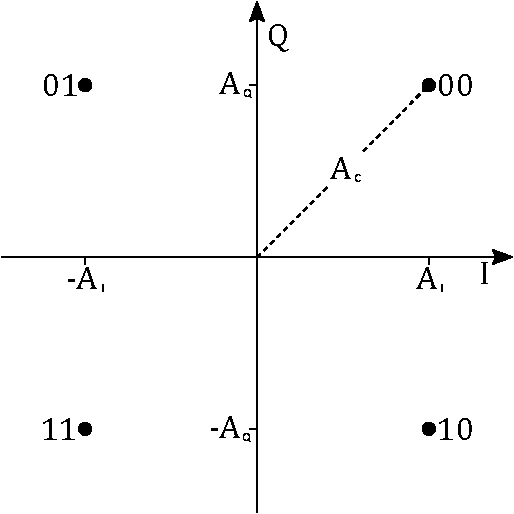
\includegraphics[width=0.5\textwidth]{./sdf/m_qam_system/figures/constellation.pdf}
	\caption{4-QAM constellation points.}
	\label{fig:const}
\end{figure}

%M can take several values: $2, 4, 16, 32, ...$. The first two correspond to BPSK and QPSK modulation, respectively.

\subsection{Theoretical Analysis}

M-QAM is a modulation scheme that takes advantage of two sinusoidal carriers with a phase difference of $\pi/2$. The resultant output consists of a signal with both amplitude and phase variations. The two carriers, referred to as I (In-phase) and Q (Quadrature), can be represented as

\begin{align}
	I(t)=a(t)\cos(\phi t) \\
	Q(t)=a(t)\sin(\phi t)
\end{align}
which means that any sinusoidal wave can be decomposed in its I and Q components:

\begin{align}
	A_c\cos(\omega~t+\phi)&=A\left(\cos(\omega~t)\cos(\phi)-\sin(\omega~t)\sin(\phi)\right) \\
	&=A_I\cos(\omega~t)-A_Q\sin(\omega~t),
\end{align}
where we have used the expression for the cosine of a sum and the definitions of $A_I$ and $A_Q$.



For the particular case of $M=4$, it can be considered that $A=A_I=A_Q$. If it is assumed there is no crosstalk or interference between the Q and I components, the signal can be treated as a pair of independent BPSK systems, one for the in-phase component and another for the quadrature component.
Using Gray coding, adjacent symbols differ by only one bit. As such, an error in a single component leads to a single bit error.
This means that the probability of an error in bit detection is independent among components, as there is no crosstalk or interference. That being the case, the bit error rate can be calculated for the BPSK case.

%Considering a signal with amplitude $A$ sampled at the signal peak with no inter-symbol interference, and affected by noise with variance $n_0/2$, the sampled value will be a Gaussian random variable with mean $\pm A$ and variance $n_0/2$. Thus, the probability of error is given by the probability that the value is affected by a deviation greater than $m$.

Let the $s(t)$ be the signal to be sampled at a given instant $t$ for either the in-phase or quadrature component, $a(t)$ be the component corresponding to the transmitted signal with peak amplitude equal to $A$, depending on whether the transmitted signal was 1 or 0, and $n(t)$ the component associated with the Gaussian white noise with spectral density $G_n(f) = n_0/2$, such that:

\begin{equation}\label{eq:sigAmpNoise}
s(t) = a(t) + n(t)
\end{equation}

\begin{figure}[H]
	\centering
	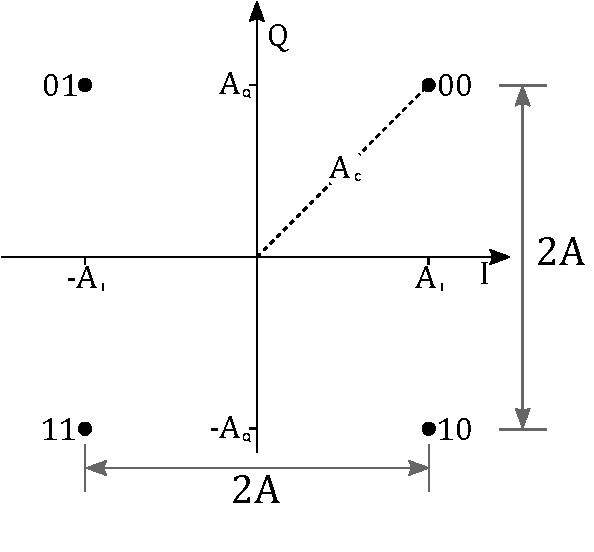
\includegraphics[width=0.5\textwidth]{./sdf/m_qam_system/figures/constellation_d.pdf}
	\caption{The relation between $A$ and the distance between constellation points.\label{fig:const_2m}}
\end{figure}

In this case, assuming the absence of inter-symbol interference, $s(t)$ at the time of sampling will be a Gaussian random variable with average value of $\pm A$, depending on what signal was transmitted, and variance equal to $N$, the noise power. In this case, using the constellation from Figure~\ref{fig:const_2m}, with a decision boundary halfway between $A$ and $-A$, an error occurs in two situations: when the a 0 is transmitted but a 1 is identified, or a 1 is transmitted and a 0 is identified. These errors happen when the perturbation in the signal due to noise is enough to push the value beyond the decision boundary. This is illustrated in Figures~\ref{fig:gauss} and~\ref{fig:gausserr}, where the probability of error is shown by the colored area under the curve~\cite{mischasch}.


\begin{figure}[H]
	\centering
	\centering
	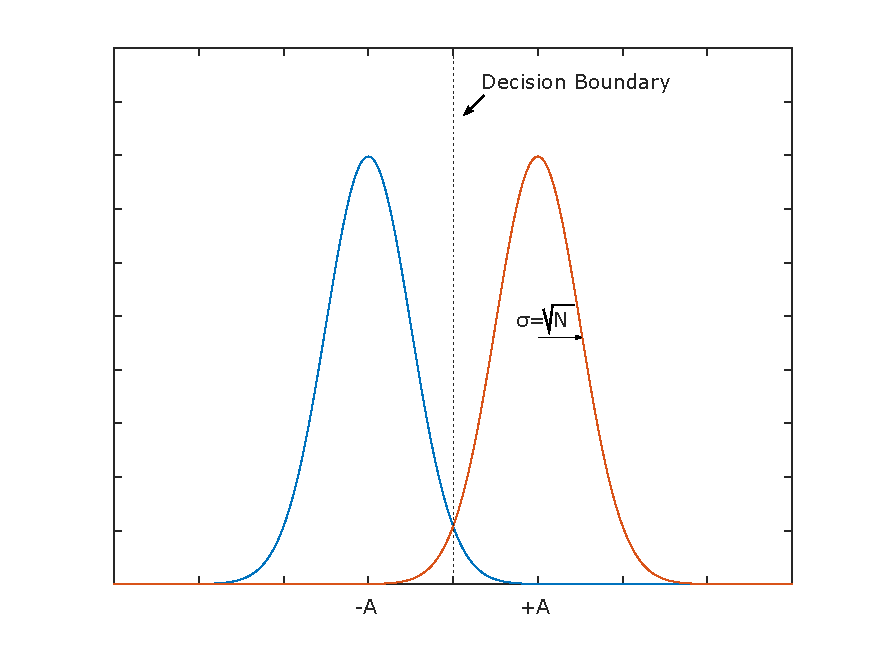
\includegraphics[ width=0.8\textwidth]{./sdf/m_qam_system/figures/gaussians.pdf}
	\caption{Probability density functions for $s(t) = a(t) + n(t)$, with $a(t)=\pm A$ and $n(t)$ as a Gaussian variable of zero mean and variance $N$.}
	\label{fig:gauss}
\end{figure}

\begin{figure}[H]
	\centering
	\begin{subfigure}{.5\textwidth}
		\centering
		\includegraphics[clip, trim=1cm 0cm 1cm 0cm,width=\textwidth]{./sdf/m_qam_system/figures/gaussian_error_2.pdf}
	\end{subfigure}%
	\begin{subfigure}{.5\textwidth}
		\centering
		\includegraphics[clip, trim=1cm 0cm 1cm 0cm,width=\textwidth]{./sdf/m_qam_system/figures/gaussian_error.pdf}
	\end{subfigure}
	\caption{The area below the curves represents the probability of error for each transmitted bit.}
	\label{fig:gausserr}
\end{figure}

The probability of bit error can be expressed as:

\begin{equation}
P_{be} = P_0 P_{e0} + P_1 P_{e1}
\end{equation}

With equal probability for both bits, and considering the constellation's symmetry

\begin{equation}\label{eq:berMQAM}
P_{be} =  Q\left({\frac{A}{\sqrt{N}}}\right) = \frac{1}{2} \text{erfc}\left({\frac{A}{\sqrt{2 N}}}\right) 
%= \frac{1}{2} \text{erfc}\left({\frac{A}{\sqrt{n_0}}}\right)
\end{equation}


%\begin{equation}
%P_b= Q\left(\sqrt{\frac{E_b}{n_0}}\right) = \frac{1}{2} erfc\left(\sqrt{\frac{E_b}{2 n_0}}\right).
%\end{equation}

%\begin{equation}\label{eq:berBPSK}
%P_{BE}= Q\left({\sqrt{\frac{2 E_b}{N_0}}}\right) = \frac{1}{2} \text{erfc}\left({\sqrt{\frac{ E_b}{N_0}}}\right).
%\end{equation}

%\begin{equation}\label{eq:berBPSK}
%BER= Q\left({G_{ele}\sqrt{\frac{2 P_L P_S}{n_0}}}\right) = \frac{1}{2} \text{erfc}\left({G_{ele}\sqrt{\frac{P_L P_S}{n_0}}}\right).
%\end{equation}

with


\begin{eqnarray}
&A &= K_{ele} \sqrt{P_L P_S}\label{eq:bpskamplitude}\\
%&N &\propto n_0 B
&N & = n_0 B\label{eq:noiseBw}
%&N & = 2 \frac{n_0}{2} B\label{eq:noiseBw}
\end{eqnarray}
%\begin{equation}\label{eq:berBPSK}
%BER= Q\left({G_{ele}\sqrt{\frac{2 P_L P_S}{n_0}}}\right) = \frac{1}{2} \text{erfc}\left({G_{ele}\sqrt{\frac{P_L P_S}{n_0}}}\right).
%\end{equation}

\noindent where $P_L$ is the local oscillator power, $P_S$ is the average optical power of the laser source on which the signal is modulated, $K_{ele}$ is the transimpedance amplifier's gain, $n_0/2$ is the noise spectral density and $B$ is the channel bandwidth. $A$ is the magnitude of the signal at sampling time and $\sqrt{N}$ is the RMS noise. Figure~\ref{fig:const_2m} shows the relation between the constellation points and $A$.

The symbol error rate depends on both bits being correctly detected. This probability is:

\begin{equation}
P_C = (1 - P_{be})^2
\end{equation}

From this, the probability of symbol error is:

\begin{eqnarray}
&P_s &= 1-P_C \nonumber\\
&	   &= 1 - \left(1 - Q \left({\frac{A}{\sqrt{N}}}\right)\right)^2 \nonumber \\
&	   &= 2 Q\left({\frac{A}{\sqrt{N}}}\right)\left[1-\frac{1}{2} Q \left({\frac{A}{\sqrt{N}}}\right)\right]
\end{eqnarray}


%$N_0$ will be the standard deviation of the sampled values.
The peak power signal-to-noise ratio, defined as the ratio between the instantaneous peak signal power to mean noise power, is given by~\cite{mischasch}:

\begin{equation}
	\text{SNR} = \frac{A^2}{{N}}
\end{equation}

\noindent 	$N$, the mean noise power, is the variance of the noise signal. The square root of this value is the peak signal-to-rms-noise ratio, and it is the single parameter on which the probability of errors depends.

\begin{equation}
\text{SNR}_{RMS} = \frac{A}{\sqrt{N}}
\end{equation}

Here, A is the peak signal amplitude and $\sqrt{N}$ is the RMS noise in the absence of a signal. Here it is assumed that the electric filter's bandwidth is large enough for the signal not to be affected. This way it only limits the noise power.

It is possible to decrease the SNR and, consequently, the error rate reducing the filter's bandwidth and finding an optimum filter. This filter is called a matched filter. The resulting signal will still have Gaussian noise, but the signal-to-noise ratio will be greatly improved. This can be achieved by using a root-raised cosine filter at the pulse shaper and a similar one at the receiver, before the sampler. Inter-symbol interference will still be null as it is equivalent to a raised cosine filter, where half the filtering is done on the transmitter side (while pulse-shaping) and the other half is done on the receiver side, before sampling.

%As the constellation remains the same, the expression to calculate the BER is similar, but replacing the values of $m$ and $N_0$ of Equation~\eqref{eq:berMQAM} by those corresponding to the signal at the output of the filter, which can be calculated as:
Considering a pulse with composition similar to the signal described by Equation~\ref{eq:sigAmpNoise}, let $ a(t) = A_p~p(t) $, where $A_p$ is the peak amplitude of the signal and $p(t)$ is the shape of the pulse, and $n(t)$ be AWGN of spectral density $G_n(f) = \frac{n_0}{2}$. Also, let $H(f)$ be the frequency domain response of the filter at the receiver.
The filter is similar to the shape of the pulse , but reversed in time and shifted by a time delay, such that it maximizes the SNR~\cite{carlson1986communication}.

The energy contained in the pulse that enters the receiver filter depends on the pulse amplitude and on its shape, and it is given by:

\begin{eqnarray}\label{eq:pulseEnergy}
E_p = \int_{-\infty}^{\infty} {|A(f)|}^2 df = A_p^2 \int_{-\infty}^{\infty} {|P(f)|}^2 df  
\end{eqnarray}

The amplitude of the signal component after the receiver filter $H(f)$, at a given sampling time $t=t_0+t_d$, is:

\begin{eqnarray}
A_o = \mathfrak{F}^{-1}\left[H(f) A(f)\right]\big|_{t=t_0+t_d} = A_p \int_{-\infty}^{+\infty} H(f) P(f) e^{+j \omega t_d}df
\end{eqnarray}

Similarly, the noise power at the receiver filter output is given by:

\begin{eqnarray}
N_o = \int_{-\infty}^{+\infty} {|H(f)|}^2 G_n(f) df = \frac{n_0}{2} \int_{-\infty}^{+\infty} {|H(f)|}^2
\end{eqnarray}

This means that the peak signal power to mean noise power ratio at the filter output is given by:

\begin{eqnarray}
\frac{A_o^2}{N_o} &= A_p^2 \frac{\big|\int_{-\infty}^{+\infty} |H(f) P(f)e^{j\omega t_d} df\big|^2}{\int_{-\infty}^{+\infty} {|H(f)|}^2 G_n(f) df}\\\nonumber
				  &= A_p^2 \frac{\big|\int_{-\infty}^{+\infty} |H(f) P(f)e^{j\omega t_d} df\big|^2}{\frac{n_0}{2}\int_{-\infty}^{+\infty} {|H(f)|}^2df}
\end{eqnarray}

It can be shown that a matched filter maximizes the ratio above, so that it becomes~\cite{carlson1986communication} :

\begin{equation}
\frac{A_o^2}{N_o} = \frac{A_p^2}{n_0/2} \int_{-\infty}^{+\infty} |P(f)|^2 df = \frac{A_p^2}{n_0/2} \int_{-\infty}^{+\infty} p(t)^2 dt
\end{equation}

Substituting from equation~\ref{eq:pulseEnergy}:

\begin{equation}
\frac{A_o^2}{N_o} = \frac{2 E_p}{n_0}
\end{equation}

This shows that the SNR and, therefore, the error probability are dependent on the energy of each symbol and the noise spectral density. However, even though the relation does not directly depend on the pulse shape, the energy of each symbol still depends on the pulse shape. The energy of the symbol results from an integration over the symbol period.
% Considering two a similar shaped pulses, with similar amplitude but duration, the one with longer duration should have more energy.

The BER expression for matched filtering the becomes:

\begin{equation}\label{eq:berMQAMmf}
P_{be} =  Q\left(\sqrt{\frac{2 E_p}{{n_0}}}\right) = \frac{1}{2} \text{erfc}\left(\sqrt{\frac{E_p}{n_0}}\right) 
%= \frac{1}{2} \text{erfc}\left({\frac{A}{\sqrt{n_0}}}\right)
\end{equation}

To exemplify with a simple case, let the pulse shape be rectangular with period $T_s$, such as:

\begin{equation*}
	a(t) = \begin{cases}
		A               & 0 \le t \le T_s\\
		0               & t > T_s\\
	\end{cases}
\end{equation*}

The energy of a pulse at the receptor input will be given by:

\begin{equation}
E_p = \int_{0}^{T_s} {a(t)^2cos^2(\omega_0 t)} dt 
\end{equation}

If $\omega_0$ is such that $\omega_0 T_s \gg 1$, as it typically is when modulating optical signals, $cos^2(\omega_0 t) \doteq 1/2$. Then:

\begin{equation}\label{eq:rectSigEn}
E_p \doteq \frac{1}{2}\int_{0}^{T_s} a(t)^2 dt = \frac{1}{2}\int_{0}^{T_s} A^2 p(t)^2 dt=\frac{1}{2} A^2 \int_{0}^{T_s} p(t)^2 dt= \frac{A^2 T_s}{2}
\end{equation}

Substituting from equations~\ref{eq:noiseBw} and~\ref{eq:rectSigEn} into Equation~\ref{eq:berMQAMmf}, the BER expression becomes:

\begin{equation}\label{eq:berMod}
P_{be} = \frac{1}{2} \text{erfc}\left(\sqrt{\frac{A^2 T_s / 2}{ N / B}}\right) = 
\frac{1}{2} \text{erfc}\left(\frac{A}{\sqrt{2N}} {{T_s}{B}}\right) 
%= \frac{1}{2} \text{erfc}\left({\frac{A}{\sqrt{n_0}}}\right)
\end{equation}

%Similarly, let the signal be shaped using a root-raised-filter, defined as the square root of a raised-cosine in the frequency domain. It ca defined as:

%\begin{equation}
%	RRC(f) = \begin{cases}
%	1              & |f| \le \frac{1-\beta}{2T_s}\\
%	1 cos\left[\frac{\pi T_s}{2 \beta}\left( |f| - \frac{1-\beta}{2T_s}\right)\right]               & \frac{1-\beta}{2T_s} \le |f| \le \frac{1+\beta}{2T_s}\\
%	0						   & |f|  \ge \frac{1+\beta}{2T_s}
%	\end{cases}
%\end{equation}
%
%The energy of a signal

%In the case of QPSK with m=4, both the quadrature and in-phase components have $a(t) = \pm A$. The values that replace $A$ and $N_0$ in Equation~\ref{eq:berMQAM} become:

%\begin{eqnarray}
%%&A_{mf} &= \frac{A T}{2} = \frac{G_{ele} T_s B \sqrt{P_L P_S}}{2}\\
%%&N_{mf} &= N \frac{T_s B}{2}
%%&A_{mf} &= \frac{A T}{2} = \frac{G_{ele} T \sqrt{P_L P_S}}{2}\\
%%&N_{mf} &= N \frac{T}{2}
%\end{eqnarray}

%Here, $P_L$ is the local oscillator power, $P_S$ is the average optical power of the laser source on which the signal is modulated, $G_{ele}$ is the gain in the transimpedance amplifier, $T_s$ is the symbol period, $B$ is the bandwidth of the system, $A_mf$ is the average amplitude at the sampling points of the signal after amplification without noise, $\sigma_o^2$ is the variance of the noise component of the matched filter output, the and $n_0$ is the noise spectral density.
%
%
%The optimal BER that can be obtained by using matched filtering is then given by:

%%\begin{eqnarray}\label{eq:berBPSK}
%&P_{be} &= Q\left({\frac{A_{mf}}{\sqrt{N_{mf}}}}\right)\nonumber\\
%&		&= \frac{1}{2} \text{erfc}\left({\frac{A_{o}}{\sqrt{2 N_{o}}}}\right)\nonumber\\
%%&	    &= \frac{1}{2} \text{erfc}\left({\frac{A}{\sqrt{N}}\sqrt{\frac{T_s B}{2}}}\right)\\
%&	    &= \frac{1}{2} \text{erfc}\left({\frac{A}{\sqrt{N}}\sqrt{\frac{T}{2}}}\right)\\
%%&	    &= \frac{1}{2} \text{erfc}\left(\sqrt{{\frac{E_b}{n_0}}}\right)\nonumber
%\end{eqnarray}

%with
%
%\begin{eqnarray}
%&A &= G_{ele} \sqrt{P_L P_S}
%%&m_{mf} &= \frac{1}{2} T G_{ele} \sqrt{P_L P_S} \\
%%&E_b &= \frac{A^2 T}{2} \\
%\end{eqnarray}


%\noindent where $T_s$ is the symbol period, $B$ is the bandwidth of the system, $A$ is as defined in Equation~\ref{eq:bpskamplitude}, the peak amplitude of the signal without noise prior to filtering.
%%and $B_e$ is the energy of a single received bit.

Note that $N$ here is the noise power at the input of the matched filter, as is the bandwidth $B$ and the peak amplitude $A$. The expressions for the Bit-Error-Rate in the cases with and without matched filtering:

\begin{table}[H]
	\centering
	\begin{tabulary}{1.0\textwidth}{|c|c|}
		\hline
		\textbf{Without matched filter} 								& \textbf{With Matched Filter} \\ \hline
		$ \frac{1}{2} \text{erfc} \left( \frac{A}{\sqrt{2N}} \right) $	& $ \frac{1}{2} \text{erfc}\left(\frac{A}{\sqrt{2N}} \sqrt{\frac{T_s}{B}}\right)  $ \\ \hline
	\end{tabulary}
	
	\caption{Comparison between the BER equations for the cases with and without matched filtering.\label{tab:ber_qpsk}}
\end{table}

Figure~\ref{fig:QPSK_th_curves} show the curves for both these equations, with the parameters listed in Table~\ref{tab:thCurves}.
%Here, $T$ is the symbol period.

\begin{table}[H]
	\centering
	\begin{tabular}{|l|l|}
		\hline
		\multicolumn{2}{|c|}{ \textbf{Curve Parameters} } \\
		\hline
		\textbf{Parameter}     & \textbf{Default Value}                                     \\\hline
		%		numberOfBitsGenerated  & $40000$	                                                \\\hline
		bandwidth              & 64 GHz															\\\hline
		symbolRate		       & 4 GHz                                                    		\\\hline
		%		samplesPerSymbol       & $16$                                                       \\\hline
		%		symbolRate		       &                                                     		\\\hline
		%		pLength                & $5$                                                        \\\hline
		%		iqAmplitudesValues     & $\lbrace~\lbrace-1,~0\rbrace~,~\lbrace1,~0\rbrace~\rbrace$ \\\hline
		outputOpticalPower     & Variable                                                   \\ \hline
		localOscillatorPower   & $0$~dBm                                                    \\ \hline
		%		localOscillatorPhase   & $0$                                                        \\ \hline
		%		transferMatrix         & $\lbrace~\lbrace \frac{1}{\sqrt{2}},~\frac{1}{\sqrt{2}},~\frac{1}{\sqrt{2}},~\frac{-1}{\sqrt{2}} \rbrace~\rbrace$ & \\ \hline
		responsivity           & $1$                                                        \\ \hline
		amplification          & $10^3$                                                     \\ \hline
		noisePower			   & $10^{-6}$~V$^2$                             					\\ \hline
		confidence             & $0.95$                                                     \\ \hline
		theoreticalSNR (before matched filter) &	0 dB								    \\ \hline
		%		midReportSize          & $0$                                                        \\ \hline
	\end{tabular}
	\caption{Parameters for the theoretical curves in Figure~\ref{fig:QPSK_th_curves}.\label{tab:thCurves}}
\end{table}

\begin{figure}[H]
	\centering
	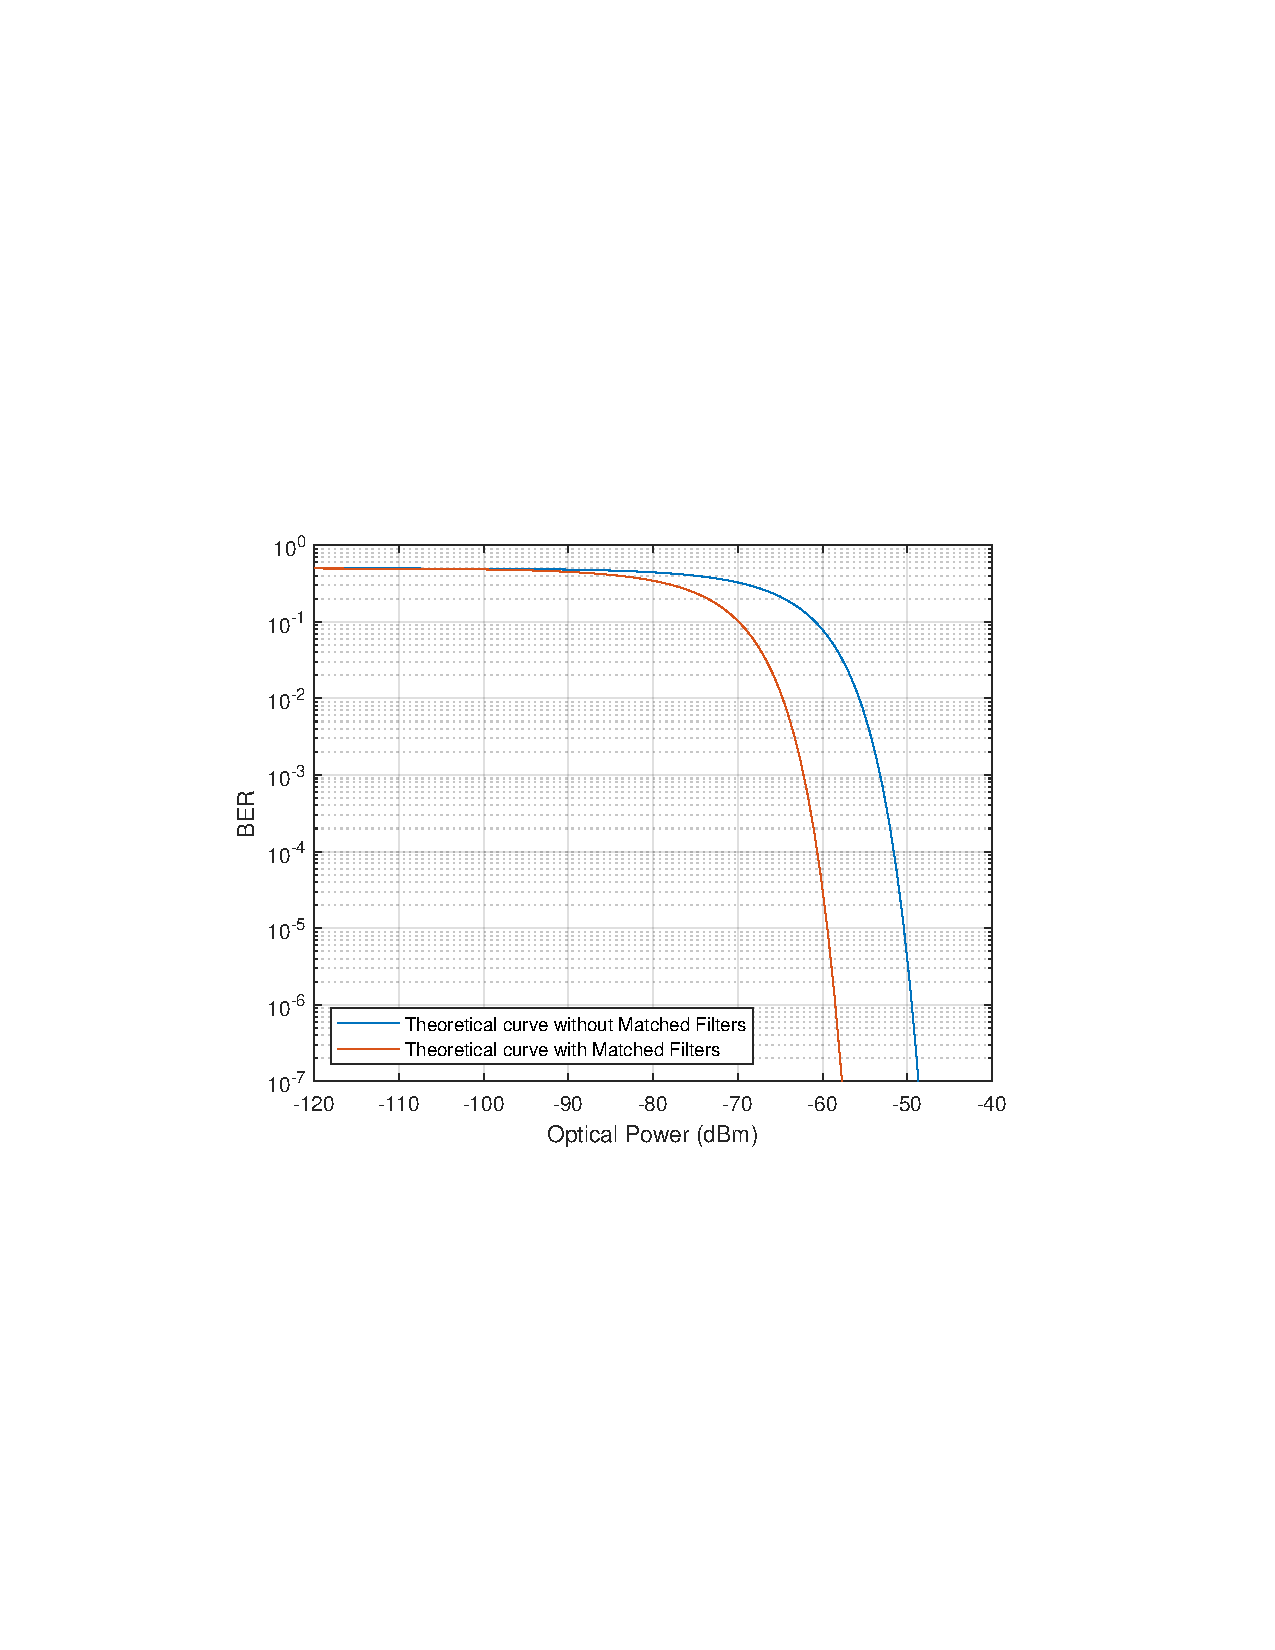
\includegraphics[clip, trim=4cm 8cm 4cm 8cm, width=0.7\textwidth]{./sdf/m_qam_system/figures/teor_BER_curves.pdf}
	\caption{QPSK theoretical BER values as a function of the output optical power in dBm.\label{fig:QPSK_th_curves}}
\end{figure}


Figure~\ref{fig:QPSK_th_curves} shows the two theoretical curves for QPSK. The blue one is for QPSK without matched filtering and the red one is using root-raised-cosine for matched filtering, which provides optimum transmission. As the use of root-raised-cosine for matched filtering maximizes the signal-to-noise ratio to its optimal value, it allows achieving the same BER with much lower optical power. On the blue curve, on the other hand, the sampling is affected by the full effect of the random noise, as there is no filtering at the receiver. Because of this, a higher optical power is required to achieve a similar BER.


It's worth noting that these equations are only valid for M=4, as in that case the system is similar to QPSK with a 4 point constellation. For $M > 4$ a different approach is required.

The use of matched filtering should allow transmission with a lower SNR to achieve the same results as a similar system, even when using a shape with no inter-symbol interference. This is due to the second filter reducing the noise impact before detection, while not causing inter-symbol interference or degradation of the signal data.

\subsection{Simulation Analysis}

\begin{figure}[h]
	\centering
	\includegraphics[width=0.8\textwidth]{./sdf/m_qam_system/figures/simulation_mqam}
	\caption{Schematic representation of the MQAM system.}\label{fig:MQAM_system_block_diagram}
\end{figure}


\begin{figure}[h]
	\centering
	\includegraphics[width=1\textwidth]{./sdf/m_qam_system/figures/simulation_tx}
	\caption{Schematic representation of the MQAM Transmitter block.}\label{fig:simulation_tx}
\end{figure}

%\begin{sidewaysfigure}[h]
%	\centering
%	\includegraphics{./sdf/m_qam_system/figures/simulation_rx}
%	\caption{Schematic representation of the Homodyne Receiver block.}\label{fig:simulation_rx}
%\end{sidewaysfigure}

\begin{figure}[h]
	\centering
	\includegraphics{./sdf/m_qam_system/figures/simulation_rx}
	\caption{Schematic representation of the Homodyne Receiver block.}\label{fig:simulation_rx}
\end{figure}

The M-QAM transmission system is a complex block of code that simulates the modulation, transmission and
demodulation of an optical signal using M-QAM modulation.
It is composed of four blocks: a transmitter, a receiver, a sink and a block that performs a Bit Error Rate (BER) measurement. The schematic representation of the
system is presented in Figures~\ref{fig:MQAM_system_block_diagram} to~\ref{fig:simulation_rx}.
	
\paragraph{Current state:} The system currently being implement is a QPSK system (M=4).

\paragraph{Future work:} Extend this block to include other values of M.

\subsection*{Functional description}

A complete description of the M-QAM transmitter and M-QAM homodyne receiver blocks can be found in the \textit{Library} chapter of this document as well as a detailed description of the independent blocks that compose these blocks.
The M-QAM transmitter generates one or two optical signals by encoding a binary string using M-QAM modulation. It also outputs a binary signal that is used to perform the BER measurement.
The M-QAM homodyne receiver accepts one input optical signal and outputs
a binary signal. It performs the M-QAM demodulation of the input signal by combining the optical signal with a local oscillator.
The demodulated optical signal is compared to the binary one produced by the transmitter in order to estimate the Bit Error Rate (BER).
The files used are summarized in tables~\ref{tab:sources} and~\ref{tab:headers}. These include all blocks and sub-blocks used and allow for the full operation of the M-QAM system.

\subsection*{Required files}\label{RequiredFilesMQAM}

\begin{table}[H]
    \centering
    \begin{tabulary}{1.0\textwidth}{|p{7.5cm}|p{5.5cm}|p{1cm}|}
        \hline
        \multicolumn{3}{|c|}{ \textbf{Source Files} } \\
        \hline
        \textbf{File}                      			 & \textbf{Comments} & \textbf{Status} \\ \hline
        add\_20171116.cpp                            &                   & \checkmark \\ \hline
        binary\_source\_20180118.cpp                 &                   & \checkmark \\ \hline
        bit\_error\_rate\_20171810.cpp               &                   & \checkmark \\ \hline
        decoder\_20180118.cpp                        &                   & \checkmark \\ \hline
        discrete\_to\_continuous\_time\_20180118.cpp &                   & \checkmark \\ \hline
        homodyne\_receiver\_20171203.cpp             & $^{1}$			 & \checkmark \\ \hline
        ideal\_amplififer\_20180118.cpp              &                   & \checkmark \\ \hline
        iq\_modulator\_20180118.cpp                  &                   & \checkmark \\ \hline
        local\_oscillator\_20180118.cpp              &                   & \checkmark \\ \hline
        m\_qam\_mapper\_20180118.cpp                 &                   & \checkmark \\ \hline
        m\_qam\_system.cpp                 			 & $^{2}$   		 & \checkmark \\ \hline
        m\_qam\_transmitter\_20180118.cpp            &                   & \checkmark \\ \hline
        netxpto\_20180118.cpp                        & $^{2}$ 			 & \checkmark \\ \hline
        optical\_hybrid\_20180118.cpp                &                   & \checkmark \\ \hline
        photodiode\_old\_20180118.cpp                &                   & \checkmark \\ \hline
        pulse\_shaper\_20180118.cpp                  &                   & \checkmark \\ \hline
        sampler\_20171119.cpp                        &                   & \checkmark \\ \hline
        sink\_20180118.cpp                           &                   & \checkmark \\ \hline
        super\_block\_interface\_20180118.cpp        & $^{2}$ 			 & \checkmark \\ \hline
        white\_noise\_20180118.cpp                   & 					 & \checkmark \\ \hline
    \end{tabulary}

    \caption{$^1$ The library entry is under a different name, \textit{m\_qam\_receiver};\\
    $^2$ No library entry as it is a main or general purpose file, not a specific block. 	 \label{tab:sources}}
\end{table}

\begin{table}[H]
    \centering
    \begin{tabulary}{1.0\textwidth}{|p{7cm}|p{6cm}|p{1cm}|}
        \hline
        \multicolumn{3}{|c|}{ \textbf{Header Files} } \\
        \hline
        \textbf{File}                      & \textbf{Comments} & \textbf{Status} \\ \hline
        add\_20171116.h                            & 			   & \checkmark \\ \hline
        binary\_source\_20180118 .h                &                   & \checkmark \\ \hline
        bit\_error\_rate\_20171810.h               &             & \checkmark \\ \hline
        decoder\_20180118.h                        &                   & \checkmark \\ \hline
        discrete\_to\_continuous\_time\_20180118.h &                   & \checkmark \\ \hline
        homodyne\_receiver\_20171203.h             & $^{1}$          & \checkmark \\ \hline
        ideal\_amplifier\_20180118.h               &                   & \checkmark \\ \hline
        iq\_modulator\_20180118.h                  &                   & \checkmark \\ \hline
        local\_oscillator\_20180118.h              &                   & \checkmark \\ \hline
        m\_qam\_mapper\_20180118.h                 &                   & \checkmark \\ \hline
        m\_qam\_transmitter\_20180118.h            &                   & \checkmark \\ \hline
        netxpto\_20180118.h                        & $^2$ 			   & \checkmark \\ \hline
        optical\_hybrid\_20180118.h                &                   & \checkmark \\ \hline
        photodiode\_old\_20180118.h                &                   & \checkmark \\ \hline
        pulse\_shaper\_20180118.h                  &                   & \checkmark \\ \hline
        sampler\_20171119.h                        &               & \checkmark \\ \hline
        sink\_20180118.h                           &                   & \checkmark \\ \hline
        super\_block\_interface\_20180118.h        & $^2$			   & \checkmark \\ \hline
        white\_noise\_20180118.h                   &                   & \checkmark \\ \hline
    \end{tabulary}
    \caption{$^1$ The library entry is under a different name, \textit{m\_qam\_receiver}\\
    $^2$ No library entry as it is a main or general purpose file, not a specific block. \label{tab:headers}}
\end{table}

%\begin{table}[]
%	\centering
%	\caption{Main system files}
%	\begin{tabular}{|c|c|c|c|ccc}
%		\cline{1-4}
%		\textbf{System blocks} & \textbf{Source file} & \textbf{Header file}  &  \textbf{Status} & \\ \cline{1-4}
%		Main & m\_qam\_system\_sdf.cpp & --- & \checkmark & \\ \cline{1-4}
%		M-QAM transmitter & m\_qam\_transmitter\_20180118.cpp & m\_qam\_transmitter\_20180118.h & \checkmark &  \\ \cline{1-4}
%		M-QAM receiver & homodyne\_receiver\_20180118.cpp & homodyne\_receiver\_20180118.h & \checkmark &  \\ \cline{1-4}
%		Sink & sink\_20180118.cpp & sink\_20180118.h &  \checkmark & \\ \cline{1-4}
%		BER estimator & bit\_error\_rate\_20171810.cpp & bit\_error\_rate\_20171810.h & \checkmark &\\ \cline{1-4}
%	\end{tabular}
%	\label{files_table}
%\end{table}

%\subsection*{Required Files}
%
%The required header and source files needed to run this system are summarized in table \ref{table:files}.
%
%\begin{table}
% 	\centering
% 	\caption{Required files}
% 	\begin{tabular}{|c|c|p{40mm}|c|ccp{40mm}c}
% 		\cline{1-4}
% 		\textbf{Header file} & \textbf{Source file} & \textbf{Description} &  \textbf{Status} & \\ \cline{1-4}
% 		add.h & add.cpp & Adds two signals.  & \checkmark &   \\ \cline{1-4}
% 		binary\_source.h & binary\_source.cpp & Produces a binary sequence. & \checkmark & \\ \cline{1-4}
% 		bit\_error\_rate.h & bit\_error\_rate.cpp & Computes the BER and writes it to a text file. & \checkmark & \\ \cline{1-4}
% 		discrete\_to\_continuous\_time.h & discrete\_to\_continuous\_time.cpp & Converts a signal from discrete in time to continuous in time. & \checkmark & \\ \cline{1-4}
% 		homodyne\_receiver.h & m\_qam\_homodyne\_receiver.cpp & & \\ \cline{1-4}
% 		ideal\_amplifier.h & ideal\_amplifier.cpp & Amplifies the signal. & \checkmark & \\ \cline{1-4}
% 		iq\_modulator.h & iq\_modulator.cpp & Divides the signal in its quadrature and in phase components & \checkmark &\\ \cline{1-4}
% 		local\_oscillator.h & local\_oscillator.cpp & & & \checkmark &\\ \cline{1-4}
% 		m\_qam\_mapper.h & m\_qam\_mapper.cpp & Maps the signal using the defined constellation & \checkmark & \\ \cline{1-4}
% 		m\_qam\_transmitter.h & m\_qam\_transmitter.cpp & & \checkmark & \\ \cline{1-4}
% 		netxpto.h & netxpto.cpp & General class that contains definition from signals and buffers. & \checkmark &\\ \cline{1-4}
% 		optical\_hybrid.h & optical\_hybrid.cpp & Implements an optical hybrid. & \checkmark & \\ \cline{1-4}
% 		photodiode\_old.h & photodiode\_old.cpp & Pair of photodiodes and current subtraction. & \checkmark & \\ \cline{1-4}
% 		pulse\_shaper.h & pulse\_shaper.cpp & Electrical filter. & \checkmark &\\ \cline{1-4}
% 		sampler\_20171119.h & sampler\_20171119.cpp & Samples the signal. & \checkmark &\\ \cline{1-4}
% 		sink.h & sink.cpp & Deletes signal. & \checkmark & \\ \cline{1-4}
% 		super\_block\_interface.h & super\_block\_interface.cpp & & \checkmark &\\ \cline{1-4}
% 		white\_noise.h & white\_noise.cpp & Generates white gaussian noise. & \checkmark &\\ \cline{1-4}
% 	\end{tabular}
% 	\label{table:files}
%\end{table}
\pagebreak
\subsection*{Input Parameters}

%The system accepts several input parameters that can be defined by the user. These are described in table \ref{table:in_par}.

\begin{table}[H]
	\centering
	\caption{Input parameters}
	\begin{tabular}{|c|c|p{70mm}|ccp{70mm}}
		\cline{1-3}
		\textbf{Parameter} & \textbf{Type} & \textbf{Description} &    \\ \cline{1-3}
		numberOfBitsGenerated & t\_integer & Determines the number of bits to be generated by the binary source  &    \\ \cline{1-3}
		samplesPerSymbol & t\_integer & Number of samples per symbol &    \\ \cline{1-3}
		prbsPatternLength & int & Determines the length of the pseudorandom sequence pattern (used only when the binary source is operated in \textit{PseudoRandom} mode) &    \\ \cline{1-3}
		bitPeriod & t\_real & Temporal interval occupied by one bit &    \\ \cline{1-3}
		rollOffFactor\_shp & t\_real & Parameter of the pulse shaper filter &    \\ \cline{1-3}
		rollOffFactor\_out & t\_real & Parameter of the output filter &    \\ \cline{1-3}
		shaperFilter & enum & Type of filter used in Pulse Shaper &    \\ \cline{1-3}
		outputFilter & enum & Type of filter used in output filter &    \\ \cline{1-3}
		seedType & enum & Method of seeding noise generators &    \\ \cline{1-3}
		seedArray & array<int,2> & Seeds to initialize noise generators &    \\ \cline{1-3}
		signalOutputPower\_dBm & t\_real & Determines the power of the output optical signal in dBm &  \\ \cline{1-3}
		numberOfBitsReceived & int &   Determines when the simulation should stop. If $-1$ then it only stops when there is no more bits to be sent&   \\ \cline{1-3}
		iqAmplitudeValues & vector<t\_iqValues> & Determines the constellation used to encode the signal in IQ space &    \\ \cline{1-3}
		symbolPeriod & double & Given by bitPeriod/samplesPerSymbol &    \\ \cline{1-3}
		localOscillatorPower\_dBm & t\_real & Power of the local oscillator &    \\ \cline{1-3}
		responsivity & t\_real & Responsivity of the photodiodes (1 corresponds to having all optical power transformed into electrical current) &    \\ \cline{1-3}
		amplification & t\_real & Amplification provided by the ideal amplifier &    \\ \cline{1-3}
		noisePower & t\_real & Average power (and variance) of the white noise &    \\ \cline{1-3}
		samplesToSkip & t\_integer & Number of samples to be skipped by the \textit{sampler} block &    \\ \cline{1-3}
		confidence & t\_real & Determines the confidence limits for the BER estimation &    \\ \cline{1-3}
		midReportSize & t\_integer &  &    \\ \cline{1-3}
		bufferLength & t\_integer & Corresponds to the number of samples that can be processed in each run of the system &    \\ \cline{1-3}
		\end{tabular}
		\label{table:in_par}
		\end{table}

\subsection*{Simulation results}

In this section we show results obtained through the simulations. The
following sections show the eye diagrams of the signal obtained at three
different points in the system: the optical signal S1, the signals after
amplifying the electrical signal and adding the Gaussian white noise HMD12 and
HMD13, and the signal after the filter in the receiver. These eye diagrams will
be shown for a variety of system configurations, with varying noise and
filters, displaying the advantages of using matched filtering with an optimal
filter.

\subsubsection{Without Noise}

These section presents the mentioned eye diagrams in configurations without any
noise added to the signal. This allows studying the effects of inter-symbol
interference caused only by the filters used at the pulse-shaper and at the
receiver,

Figure~\ref{fig:eyespower} shows the eye diagrams for the S1 optical signals
for two different values of the output optical power. These were obtained using
a
raised-cosine filter as a pulse shaper, with a roll-off factor of 0.9. It can
be seen that no inter-symbol interference is present.

\begin{table}[H]
			\centering
			\footnotesize
	\begin{tabular}{|l|l|}
		\hline
		\multicolumn{2}{|c|}{ \textbf{Curve Parameters} } \\
		\hline
		\textbf{Parameter}     & \textbf{Default Value}                                     \\\hline
		%		numberOfBitsGenerated  & $40000$	                                                \\\hline
		bitPeriod              & $1/50\times10^9$~s														\\\hline
%		symbolRate		       &                                                     		\\\hline
		samplesPerSymbol       & $16$                                                       \\\hline
		%		symbolRate		       &                                                     		\\\hline
		%		pLength                & $5$                                                        \\\hline
		%		iqAmplitudesValues     & $\lbrace~\lbrace-1,~0\rbrace~,~\lbrace1,~0\rbrace~\rbrace$ \\\hline
		outputOpticalPower     & $-120$~dBm (left), $-60$~dBm (right)                       \\ \hline
		shaperFilter	       & RaisedCosine												\\ \hline
		rollOffFactor		   & 0.9														\\ \hline
%		localOscillatorPower   & $0$~dBm                                                    \\ \hline
		%		localOscillatorPhase   & $0$                                                        \\ \hline
		%		transferMatrix         & $\lbrace~\lbrace \frac{1}{\sqrt{2}},~\frac{1}{\sqrt{2}},~\frac{1}{\sqrt{2}},~\frac{-1}{\sqrt{2}} \rbrace~\rbrace$ & \\ \hline
%		responsivity           & $1$                                                        \\ \hline
%		amplification          & $10^3$                                                     \\ \hline
%		noisePower   & $0$~V$^2$                             					\\ \hline
%		confidence             & $0.95$                                                     \\ \hline
		%		midReportSize          & $0$                                                        \\ \hline
		
	\end{tabular}
\end{table}

\begin{figure}[H]
	\centering
	\textbf{Raised-Cosine Signal (roll-off=0.9) At the Transmitter Output}
	\begin{subfigure}{.5\textwidth}
		\centering
		\includegraphics[clip, trim=5cm 7cm 5cm 7cm,
			width=\textwidth]{./sdf/m_qam_system/figures/eye120db09ro.pdf}
	\end{subfigure}%
	\begin{subfigure}{.5\textwidth}
		\centering
		\includegraphics[clip, trim=5cm 7cm 5cm 7cm,
			width=\textwidth]{./sdf/m_qam_system/figures/eye60db09ro.pdf}
	\end{subfigure}
%	\caption{Eye diagrams for the optical signal at the transmitter output, with an output optical power
%		of $-120~dBm$ (left) and $-60~dBm$ (right) with no added noise. In this case, a raised cosine filter with a roll-off factor of 0.9 was used at the transmitter to shape the signal.}
	\caption{\label{fig:eyespower}}
\end{figure}

As mentioned previously, using matched filters is highly beneficial, as it
allows achieving much lower error rates with the same optical power.

Figure~\ref{fig:eyes_nn_rc_09} shows the eye diagrams of the signal at the
three mentioned points, for a system without any added white noise, while using
matched filtering. The filter used in this case is a raised cosine filter with
a roll-off factor of 0.9. Although this is the ideal filter to use for pulse
shaping, as it does not cause inter-symbol-interference, it can be seen that
when used twice its results are less than ideal, as shown in the eye diagram
captured after the second filter.
\begin{table}[H]
	\centering
	\footnotesize
	\begin{tabular}{|l|l|}
		\hline
		\multicolumn{2}{|c|}{ \textbf{Simulation Parameters} } \\
		\hline
		\textbf{Parameter}     & \textbf{Default Value}                                     \\\hline
		%		numberOfBitsGenerated  & $40000$	                                                \\\hline
		bitPeriod              & $1/50\times10^9$~s														\\\hline
		%		symbolRate		       &                                                     		\\\hline
		samplesPerSymbol       & $16$                                                       \\\hline
		%		symbolRate		       &                                                     		\\\hline
		%		pLength                & $5$                                                        \\\hline
		%		iqAmplitudesValues     & $\lbrace~\lbrace-1,~0\rbrace~,~\lbrace1,~0\rbrace~\rbrace$ \\\hline
		outputOpticalPower     & $-60$~dBm 													\\ \hline
		shaperFilter	       & RaisedCosine												\\ \hline
		outputFilter		   & RaisedCosine												\\ \hline
		rollOffFactor		   & 0.9														\\ \hline
				localOscillatorPower   & $0$~dBm                                                    \\ \hline
				localOscillatorPhase   & $0$                                                        \\ \hline
		%		transferMatrix         & $\lbrace~\lbrace \frac{1}{\sqrt{2}},~\frac{1}{\sqrt{2}},~\frac{1}{\sqrt{2}},~\frac{-1}{\sqrt{2}} \rbrace~\rbrace$ & \\ \hline
				responsivity           & $1$                                                        \\ \hline
				amplification          & $10^3$                                                     \\ \hline
				noisePower   & $0$~V$^2$                             					\\ \hline
		%		confidence             & $0.95$                                                     \\ \hline
		%		midReportSize          & $0$                                                        \\ \hline
	\end{tabular}
\end{table}
\begin{figure}[H]
	\centering
	\textbf{Raised-Cosine Signal (roll-off=0.9) with Matched Filtering}
	\begin{minipage}{\linewidth}
		\centering
	\begin{subfigure}{.45\textwidth}
		\centering
		\includegraphics[clip, trim=5cm 4cm 5cm 4cm,
			width=\textwidth]{./sdf/m_qam_system/figures/eyes/if_nn_p_60_09_rc.pdf}
	\end{subfigure}
	\begin{subfigure}{.45\textwidth}
		\centering
		\includegraphics[clip, trim=5cm 4cm 5cm 4cm,
			width=\textwidth]{./sdf/m_qam_system/figures/eyes/q_nn_p_60_09_rc.pdf}
	\end{subfigure}
	
	\caption{
%		Eye diagrams of the signal using matched filtering with raised-cosine without AWGN.
		Obtained at
		three different points in the system: optical output of transmitter on the top;
		the amplified signal at the middle; and
		after the receiver filter.
%		Simulation done with an optical power output of
%		-60~dBm, 0~dBm at the local oscillator, a gain of $10^3$ at the amplifier, and
%		a rolloff factor of 0.9.
		\label{fig:eyes_nn_rc_09}}
	\end{minipage}
\end{figure}

The optimum solution to achieving no inter-symbol interference while using
matched filtering is to use a root-raised-cosine to do the pulse-shaping at the
transmitter and the filtering at the receiver. The corresponding output of
applying twice a root-raised-cosine is exactly the same as using a
raised-cosine once. As such, the end result suffers from no inter-symbol
interference while reaping the benefits of optimum matched filtering.
Figure~\ref{fig:eyes_nn_rrc_09} shows the eye diagrams when using
root-raised-cosine filter both in the transmitter's pulse-shaper and at the
receiver's filter. The roll-off factor used in both was 0.9. It can be seen
that the shape of the eye diagram is equal to that of
Figure~\ref{fig:eyespower}, which uses a single raised cosine filter at the
pulse-shaper. Thus, it shows no sign of inter-symbol interference.
\begin{table}[H]
	\centering
	\footnotesize
	\begin{tabular}{|l|l|}
		\hline
		\multicolumn{2}{|c|}{ \textbf{Simulation Parameters} } \\
		\hline
		\textbf{Parameter}     & \textbf{Default Value}                                     \\\hline
		%		numberOfBitsGenerated  & $40000$	                                                \\\hline
		bitPeriod              & $1/50\times10^9$~s														\\\hline
		%		symbolRate		       &                                                     		\\\hline
		samplesPerSymbol       & $16$                                                       \\\hline
		%		symbolRate		       &                                                     		\\\hline
		%		pLength                & $5$                                                        \\\hline
		%		iqAmplitudesValues     & $\lbrace~\lbrace-1,~0\rbrace~,~\lbrace1,~0\rbrace~\rbrace$ \\\hline
		outputOpticalPower     & $-60$~dBm 													\\ \hline
		shaperFilter	       & RootRaisedCosine												\\ \hline
		outputFilter		   & RootRaisedCosine												\\ \hline
		rollOffFactor		   & 0.9														\\ \hline
		localOscillatorPower   & $0$~dBm                                                    \\ \hline
		localOscillatorPhase   & $0$                                                        \\ \hline
		%		transferMatrix         & $\lbrace~\lbrace \frac{1}{\sqrt{2}},~\frac{1}{\sqrt{2}},~\frac{1}{\sqrt{2}},~\frac{-1}{\sqrt{2}} \rbrace~\rbrace$ & \\ \hline
		responsivity           & $1$                                                        \\ \hline
		amplification          & $10^3$                                                     \\ \hline
		noisePower   & $0$~V$^2$                             					\\ \hline
		%		confidence             & $0.95$                                                     \\ \hline
		%		midReportSize          & $0$                                                        \\ \hline
	\end{tabular}
\end{table}
\begin{figure}[H]
	\centering

	\textbf{Root-Raised-Cosine Signal (roll-off=0.9) with Matched Filtering}
	\begin{minipage}{\linewidth}
		\centering
	\begin{subfigure}{.45\textwidth}
		\centering
		\includegraphics[clip, trim=5cm 4cm 5cm 4cm,
			width=\textwidth]{./sdf/m_qam_system/figures/eyes/if_nn_p_60_09.pdf}
	\end{subfigure}
	\begin{subfigure}{.45\textwidth}
		\centering
		\includegraphics[clip, trim=5cm 4cm 5cm 4cm,
			width=\textwidth]{./sdf/m_qam_system/figures/eyes/q_nn_p_60_09.pdf}
	\end{subfigure}
	\caption{
%		Eye diagrams using matched filtering with root-raised-cosine without AWGN.
		Obtained at
		three different points in the system: optical output of transmitter on the top;
		the amplified signal at the middle; and
		after the receiver filter.
%		Simulation done with an optical power output
%		of -60~dBm, 0~dBm at the local oscillator, a gain of $10^3$ at the amplifier,
%		and a rolloff factor of 0.9.
		\label{fig:eyes_nn_rrc_09}}
	\end{minipage}
	
\end{figure}

Figures~\ref{fig:eyes_nn_rrc_03} and~\ref{fig:eyes_nn_rrc_03} show a similar
comparison between matched filtering using raised-cosine or root-raised-cosine
filters, but with a roll-off factor of 0.3. Again, it can be seen that the
final shape of the eye diagram when using the root-raised-cosine for matched
filtering is the same as the shape of the optical signal S1 when using a
raised-cosine-filter.
\begin{table}[H]
	\centering
	\footnotesize
	\begin{tabular}{|l|l|}
		\hline
		\multicolumn{2}{|c|}{ \textbf{Simulation Parameters} } \\
		\hline
		\textbf{Parameter}     & \textbf{Default Value}                                     \\\hline
		%		numberOfBitsGenerated  & $40000$	                                                \\\hline
		bitPeriod              & $1/50\times10^9$~s														\\\hline
		%		symbolRate		       &                                                     		\\\hline
		samplesPerSymbol       & $16$                                                       \\\hline
		%		symbolRate		       &                                                     		\\\hline
		%		pLength                & $5$                                                        \\\hline
		%		iqAmplitudesValues     & $\lbrace~\lbrace-1,~0\rbrace~,~\lbrace1,~0\rbrace~\rbrace$ \\\hline
		outputOpticalPower     & $-60$~dBm 													\\ \hline
		shaperFilter	       & RaisedCosine												\\ \hline
		outputFilter		   & RaisedCosine												\\ \hline
		rollOffFactor		   & 0.3														\\ \hline
		localOscillatorPower   & $0$~dBm                                                    \\ \hline
		localOscillatorPhase   & $0$                                                        \\ \hline
		%		transferMatrix         & $\lbrace~\lbrace \frac{1}{\sqrt{2}},~\frac{1}{\sqrt{2}},~\frac{1}{\sqrt{2}},~\frac{-1}{\sqrt{2}} \rbrace~\rbrace$ & \\ \hline
		responsivity           & $1$                                                        \\ \hline
		amplification          & $10^3$                                                     \\ \hline
		noisePower   & $0$~V$^2$                             					\\ \hline
		%		confidence             & $0.95$                                                     \\ \hline
		%		midReportSize          & $0$                                                        \\ \hline
	\end{tabular}
\end{table}
\begin{figure}[H]
	
		\centering
	\textbf{Raised-Cosine Signal (roll-off=0.3) with Matched Filtering}
	\begin{minipage}{\linewidth}
		\centering
	\begin{subfigure}{.45\textwidth}
		\centering
		\includegraphics[clip, trim=5cm 4cm 5cm 4cm,
			width=\textwidth]{./sdf/m_qam_system/figures/eyes/if_nn_p_60_03_rc.pdf}
	\end{subfigure}
	\begin{subfigure}{.45\textwidth}
		\centering
		\includegraphics[clip, trim=5cm 4cm 5cm 4cm,
			width=\textwidth]{./sdf/m_qam_system/figures/eyes/q_nn_p_60_03_rc.pdf}
	\end{subfigure}
	
	\caption{
%		Eye diagrams using matched filtering with raised-cosine without AWGN.
		Obtained at
		three different points in the system: optical output of transmitter on the top;
		the amplified signal at the middle; and
		after the receiver filter.
%		Simulation done with an optical power output of
%		-60~dBm, 0~dBm at the local oscillator, a gain of $10^3$ at the amplifier, and
%		a rolloff factor of 0.3.
		\label{fig:eyes_nn_rc_03}}
	\end{minipage}
\end{figure}

\begin{table}[H]
	\centering
	\footnotesize
	\begin{tabular}{|l|l|}
		\hline
		\multicolumn{2}{|c|}{ \textbf{Simulation Parameters} } \\
		\hline
		\textbf{Parameter}     & \textbf{Default Value}                                     \\\hline
		%		numberOfBitsGenerated  & $40000$	                                                \\\hline
		bitPeriod              & $1/50\times10^9$~s														\\\hline
		%		symbolRate		       &                                                     		\\\hline
		samplesPerSymbol       & $16$                                                       \\\hline
		%		symbolRate		       &                                                     		\\\hline
		%		pLength                & $5$                                                        \\\hline
		%		iqAmplitudesValues     & $\lbrace~\lbrace-1,~0\rbrace~,~\lbrace1,~0\rbrace~\rbrace$ \\\hline
		outputOpticalPower     & $-60$~dBm 													\\ \hline
		shaperFilter	       & RootRaisedCosine												\\ \hline
		outputFilter		   & RootRaisedCosine												\\ \hline
		rollOffFactor		   & 0.3														\\ \hline
		localOscillatorPower   & $0$~dBm                                                    \\ \hline
		localOscillatorPhase   & $0$                                                        \\ \hline
		%		transferMatrix         & $\lbrace~\lbrace \frac{1}{\sqrt{2}},~\frac{1}{\sqrt{2}},~\frac{1}{\sqrt{2}},~\frac{-1}{\sqrt{2}} \rbrace~\rbrace$ & \\ \hline
		responsivity           & $1$                                                        \\ \hline
		amplification          & $10^3$                                                     \\ \hline
		noisePower   & $0$~V$^2$                             					\\ \hline
		%		confidence             & $0.95$                                                     \\ \hline
		%		midReportSize          & $0$                                                        \\ \hline
	\end{tabular}
\end{table}
\begin{figure}[H]
		\centering
	\textbf{Root-Raised-Cosine Signal (roll-off=0.3) with Matched Filtering}
	\begin{minipage}{\linewidth}
		\centering
	\begin{subfigure}{.45\textwidth}
		\centering
		\includegraphics[clip, trim=5cm 4cm 5cm 4cm,
			width=\textwidth]{./sdf/m_qam_system/figures/eyes/if_nn_p_60_03.pdf}
	\end{subfigure}
	\begin{subfigure}{.45\textwidth}
		\centering
		\includegraphics[clip, trim=5cm 4cm 5cm 4cm,
			width=\textwidth]{./sdf/m_qam_system/figures/eyes/q_nn_p_60_03.pdf}
	\end{subfigure}
	
	\caption{
%		Eye diagrams using matched filtering with root-raised-cosine without AWGN.
		Obtained at
		three different points in the system: optical output of transmitter on the top;
		the amplified signal at the middle; and
		after the receiver filter.
%		Simulation done with an optical power output
%		of -60~dBm, 0~dBm at the local oscillator, a gain of $10^3$ at the amplifier,
%		and a rolloff factor of 0.3.
		\label{fig:eyes_nn_rrc_03}}
	\end{minipage}
	
\end{figure}

Thus, it can be concluded that, in order to avoid inter-symbol interference,
the filters used should be raised-cosine or root-raised-cosine, if not using a
filter at the receiver or if using matched filtering, respectively. As such,
from now on only these configurations will be used.

\subsubsection*{With Noise (High SNR)}

In this section and the following one, a comparison will be presented between
not using a filter on the receiver and using matched filtering. This comparison
will be made for signals affected by added white gaussian noise, where the
noise is added to the signal after the amplifier stage and before the signal
passes through the filter on the receiver.

For the first case, where no filter is present at the receiver, a
raised-cosine filter will be used at the pulse shaper. For matched filtering, a
root-raised-cosine filter will be used at the pulse-shaper and the receiver.

Figures \ref{fig:eyes_n_rc_45_09}-\ref{fig:eyes_n_rrc_45_09} show the eye
diagrams for both these cases. The optical power used was $-45~dBm$, the
noise power was set at $10^{-6} V^2$, and the roll-off factor was set
to $0.9$ in both cases. In both cases, its is still possible to visibly see the
approximate shape of the signal after noise is added, even without matched
filtering. However, it can be seen that the output signal in the case with
matched filtering is much less affected by noise, as the root-raised-cosine at
the receiver is rather effective at filtering the noise.

\begin{table}[H]
	\centering
	\footnotesize
	\begin{tabular}{|l|l|}
		\hline
		\multicolumn{2}{|c|}{ \textbf{Simulation Parameters} } \\
		\hline
		\textbf{Parameter}     & \textbf{Default Value}                                     \\\hline
		%		numberOfBitsGenerated  & $40000$	                                                \\\hline
		bitPeriod              & $1/50\times10^9$~s														\\\hline
		%		symbolRate		       &                                                     		\\\hline
		samplesPerSymbol       & $16$                                                       \\\hline
		%		symbolRate		       &                                                     		\\\hline
		%		pLength                & $5$                                                        \\\hline
		%		iqAmplitudesValues     & $\lbrace~\lbrace-1,~0\rbrace~,~\lbrace1,~0\rbrace~\rbrace$ \\\hline
		outputOpticalPower     & $-45$~dBm 													\\ \hline
		shaperFilter	       & RaisedCosine												\\ \hline
		outputFilter		   & 															\\ \hline
		rollOffFactor		   & 0.9														\\ \hline
		localOscillatorPower   & $0$~dBm                                                    \\ \hline
		localOscillatorPhase   & $0$                                                        \\ \hline
		%		transferMatrix         & $\lbrace~\lbrace \frac{1}{\sqrt{2}},~\frac{1}{\sqrt{2}},~\frac{1}{\sqrt{2}},~\frac{-1}{\sqrt{2}} \rbrace~\rbrace$ & \\ \hline
		responsivity           & $1$                                                        \\ \hline
		amplification          & $10^3$                                                     \\ \hline
		noisePower   & $10^{-6}$~V$^2$                             					\\ \hline
		%		confidence             & $0.95$                                                     \\ \hline
		%		midReportSize          & $0$                                                        \\ \hline
		theoreticalSNR  	   & $15~dB$                             					\\ \hline
		numericalSNR 		   & $13.9182~dB$                             					\\ \hline
		numericalSNR Upper Bound (95\% confidence) & $13.9624~dB$                             					\\ \hline
		numericalSNR Lower Bound (95\% confidence) & $13.8737~dB$                             					\\ \hline
	\end{tabular}
\end{table}
\begin{figure}[H]
		\centering
	\textbf{Raised-Cosine Signal (roll-off=0.9) with Added Noise, SNR = 15 dB}
	\begin{minipage}{\linewidth}
		\centering
	\begin{subfigure}{.45\textwidth}
		\centering
		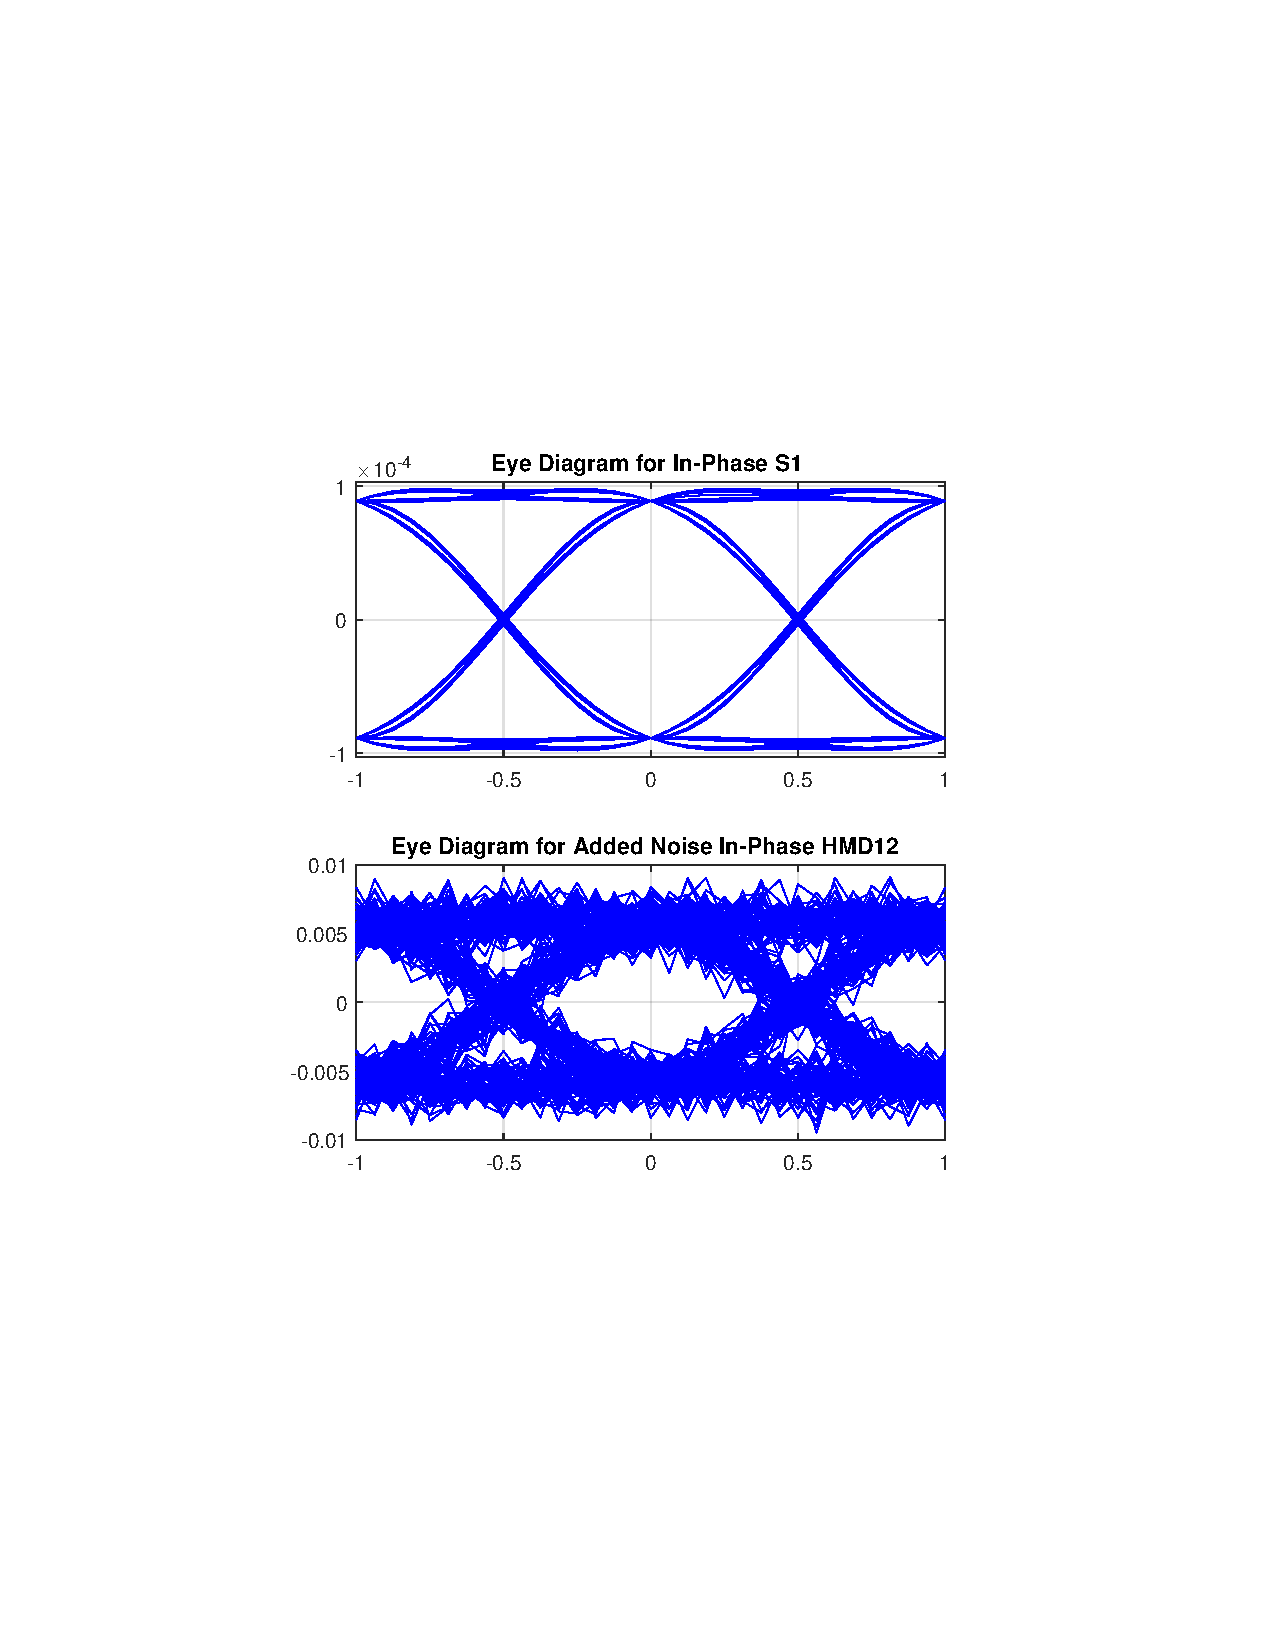
\includegraphics[clip, trim=5cm 7cm 5cm 7cm, width=\textwidth]{./sdf/m_qam_system/figures/eyes/if_n_nmf_45_60_rc_09.pdf}
	\end{subfigure}
	\begin{subfigure}{.45\textwidth}
		\centering
		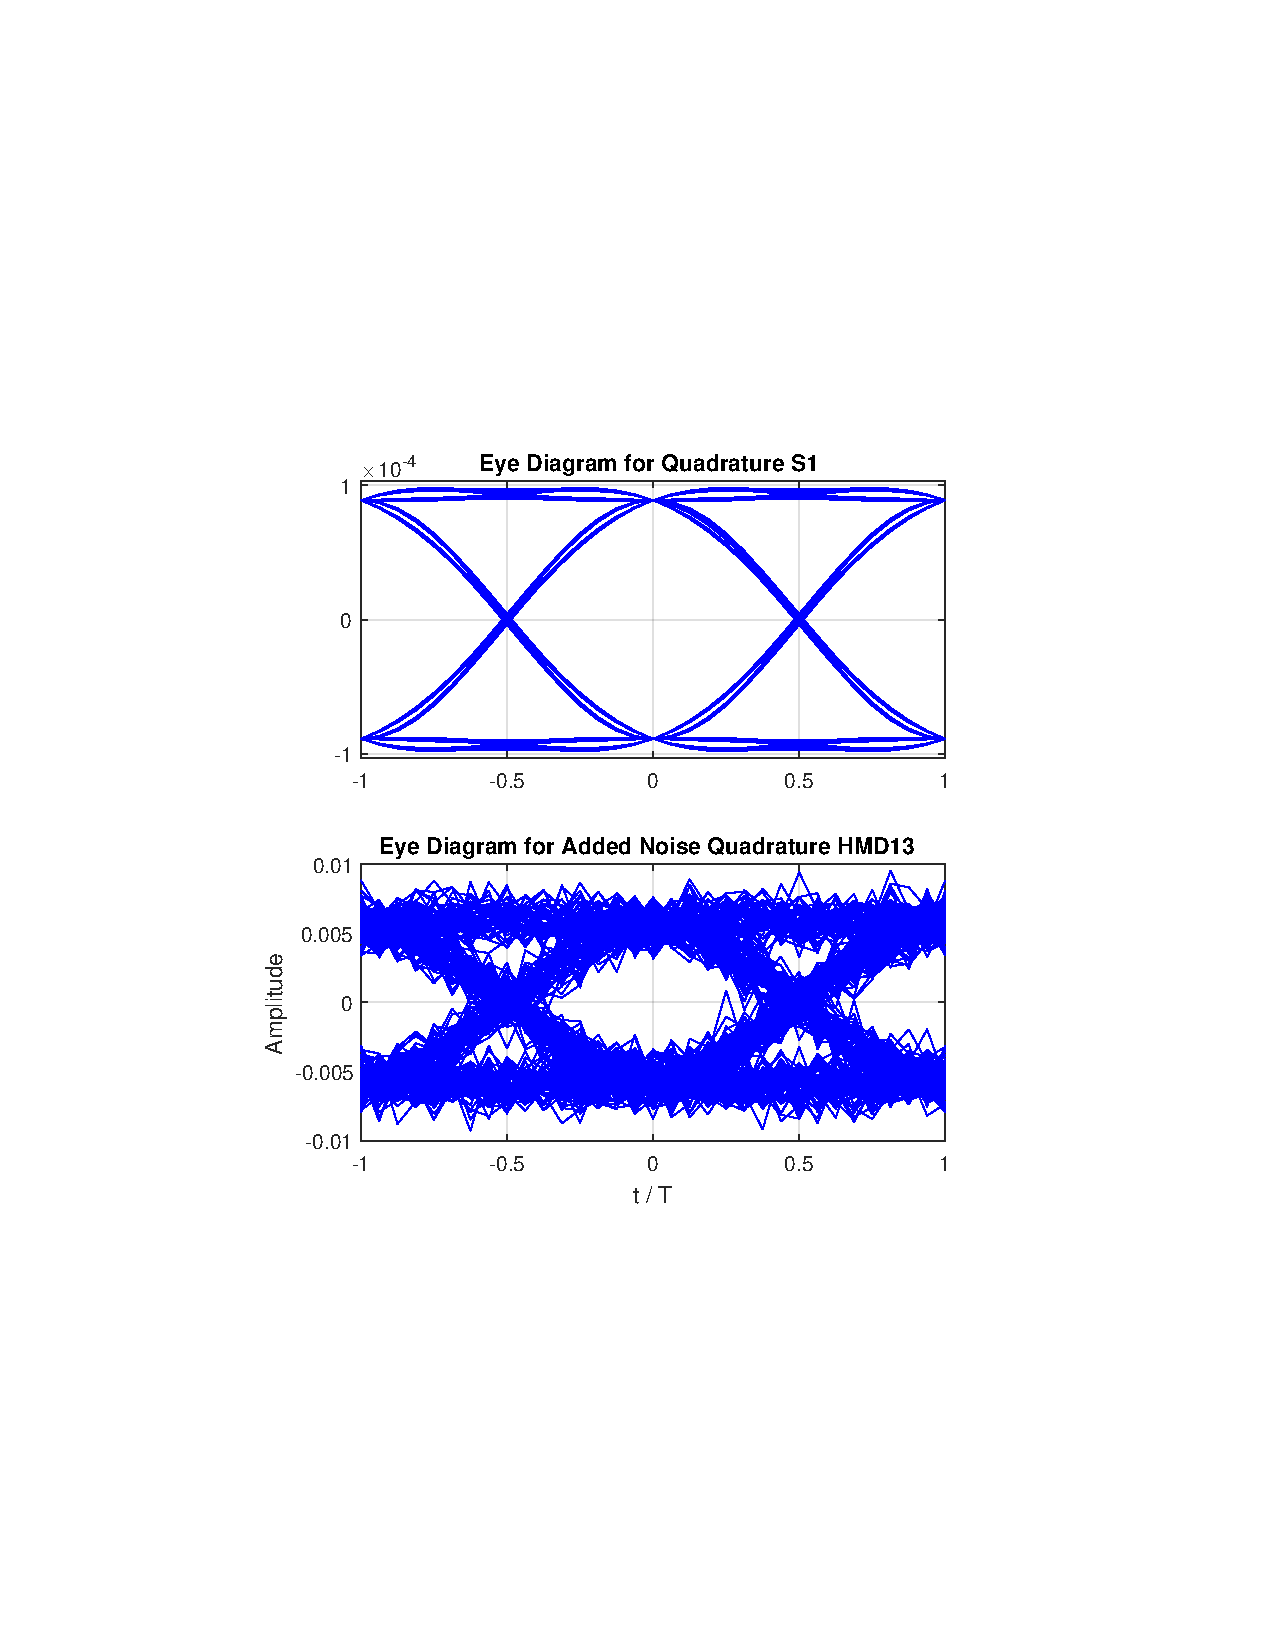
\includegraphics[clip, trim=5cm 7cm 5cm 7cm, width=\textwidth]{./sdf/m_qam_system/figures/eyes/q_n_nmf_45_60_rc_09.pdf}
	\end{subfigure}
	
	\caption{
%		Eye diagrams without matched filtering using raised-cosine.
		Obtained
		at two different points in the system: optical output of transmitter on the top and
		the noisy signal at the bottom.
%		Obtained through simulation with an optical power output of
%		-45~dBm, 0~dBm at the local oscillator, a gain of $10^3$ at the amplifier, a
%		noise spectral density of $10^{-6}$ and a rolloff factor of
%		0.9.
		\label{fig:eyes_n_rc_45_09}}
	\end{minipage}
\end{figure}
\begin{table}[H]
	\centering
	\footnotesize
	\begin{tabular}{|l|l|}
		\hline
		\multicolumn{2}{|c|}{ \textbf{Simulation Parameters} } \\
		\hline
		\textbf{Parameter}     & \textbf{Default Value}                                     \\\hline
		%		numberOfBitsGenerated  & $40000$	                                                \\\hline
		bitPeriod              & $1/50\times10^9$~s														\\\hline
		%		symbolRate		       &                                                     		\\\hline
		samplesPerSymbol       & $16$                                                       \\\hline
		%		symbolRate		       &                                                     		\\\hline
		%		pLength                & $5$                                                        \\\hline
		%		iqAmplitudesValues     & $\lbrace~\lbrace-1,~0\rbrace~,~\lbrace1,~0\rbrace~\rbrace$ \\\hline
		outputOpticalPower     & $-45$~dBm 													\\ \hline
		shaperFilter	       & RootRaisedCosine												\\ \hline
		outputFilter		   & RootRaisedCosine												\\ \hline
		rollOffFactor		   & 0.9														\\ \hline
		localOscillatorPower   & $0$~dBm                                                    \\ \hline
		localOscillatorPhase   & $0$                                                        \\ \hline
		%		transferMatrix         & $\lbrace~\lbrace \frac{1}{\sqrt{2}},~\frac{1}{\sqrt{2}},~\frac{1}{\sqrt{2}},~\frac{-1}{\sqrt{2}} \rbrace~\rbrace$ & \\ \hline
		responsivity           & $1$                                                        \\ \hline
		amplification          & $10^3$                                                     \\ \hline
		noisePower   & $10^{-6}$~V$^2$                             					\\ \hline
		theoreticalSNR  	   & $15~dB$                             					\\ \hline
		numericalSNR 		     & $14.9902~dB$                             					\\ \hline
		numericalSNR Upper Bound (95\% confidence) & $15.0408~dB$                             					\\ \hline
		numericalSNR Lower Bound (95\% confidence) & $14.9391~dB$                             					\\ \hline
		%		confidence             & $0.95$                                                     \\ \hline
		%		midReportSize          & $0$                                                        \\ \hline
	\end{tabular}
\end{table}
\begin{figure}[H]
	\centering
\textbf{Root-Raised-Cosine Signal (roll-off=0.9) with Added Noise and Matched Filtering,\\SNR = 15}
\begin{minipage}{\linewidth}
	\centering
	\begin{subfigure}{.45\textwidth}
		\centering
			\includegraphics[clip, trim=5cm 4cm 5cm 4cm, width=\textwidth]{./sdf/m_qam_system/figures/eyes/if_p_45_09.pdf}
	\end{subfigure}
	\begin{subfigure}{.45\textwidth}
		\centering
		\includegraphics[clip, trim=5cm 4cm 5cm 4cm, width=\textwidth]{./sdf/m_qam_system/figures/eyes/q_p_45_09.pdf}
	\end{subfigure}
	
	\caption{
%		Eye diagrams using matched filtering with root-raised-cosine.
		Obtained at three different points in the system: optical output of transmitter on the top;
		the amplified signal at the middle; and
		after the receiver filter.
%		Simulation done with an optical
%		power output of -45~dBm, 0~dBm at the local oscillator, a gain of $10^3$ at the
%		amplifier, a noise spectral density of $10^{-6}$ and a rolloff factor of
%		0.9.
		\label{fig:eyes_n_rrc_45_09}}
	\end{minipage}
\end{figure}


Figures~\ref{fig:eyes_n_rc_45_03} and~\ref{fig:eyes_n_rrc_45_03} show the
cases described above, but with a roll-off factor of 0.3. It can be seen that
the case is in all aspects similar to the one presented above.

\begin{table}[H]
	\centering
	\footnotesize
	\begin{tabular}{|l|l|}
		\hline
		\multicolumn{2}{|c|}{ \textbf{Simulation Parameters} } \\
		\hline
		\textbf{Parameter}     & \textbf{Default Value}                                     \\\hline
		%		numberOfBitsGenerated  & $40000$	                                                \\\hline
		bitPeriod              & $1/50\times10^9$~s														\\\hline
		%		symbolRate		       &                                                     		\\\hline
		samplesPerSymbol       & $16$                                                       \\\hline
		%		symbolRate		       &                                                     		\\\hline
		%		pLength                & $5$                                                        \\\hline
		%		iqAmplitudesValues     & $\lbrace~\lbrace-1,~0\rbrace~,~\lbrace1,~0\rbrace~\rbrace$ \\\hline
		outputOpticalPower     & $-45$~dBm 													\\ \hline
		shaperFilter	       & RaisedCosine												\\ \hline
		outputFilter		   &                     										\\ \hline
		rollOffFactor		   & 0.3														\\ \hline
		localOscillatorPower   & $0$~dBm                                                    \\ \hline
		localOscillatorPhase   & $0$                                                        \\ \hline
		%		transferMatrix         & $\lbrace~\lbrace \frac{1}{\sqrt{2}},~\frac{1}{\sqrt{2}},~\frac{1}{\sqrt{2}},~\frac{-1}{\sqrt{2}} \rbrace~\rbrace$ & \\ \hline
		responsivity           & $1$                                                        \\ \hline
		amplification          & $10^3$                                                     \\ \hline
		noisePower   & $10^{-6}$~V$^2$                             					\\ \hline
		theoreticalSNR  	   & $15~dB$                             					\\ \hline
				numericalSNR 		     & $14.6827~dB$                             					\\ \hline
		numericalSNR Upper Bound (95\% confidence) & $14.7321~dB$                             					\\ \hline
		numericalSNR Lower Bound (95\% confidence) & $14.6327~dB$                             					\\ \hline
		%		confidence             & $0.95$                                                     \\ \hline
		%		midReportSize          & $0$                                                        \\ \hline
	\end{tabular}
\end{table}
\begin{figure}[H]
		\centering
	\textbf{Raised-Cosine Signal (roll-off=0.3) with Added Noise, SNR = 15 dB}
	\begin{minipage}{\linewidth}
		\centering
	\begin{subfigure}{.45\textwidth}
		\centering
		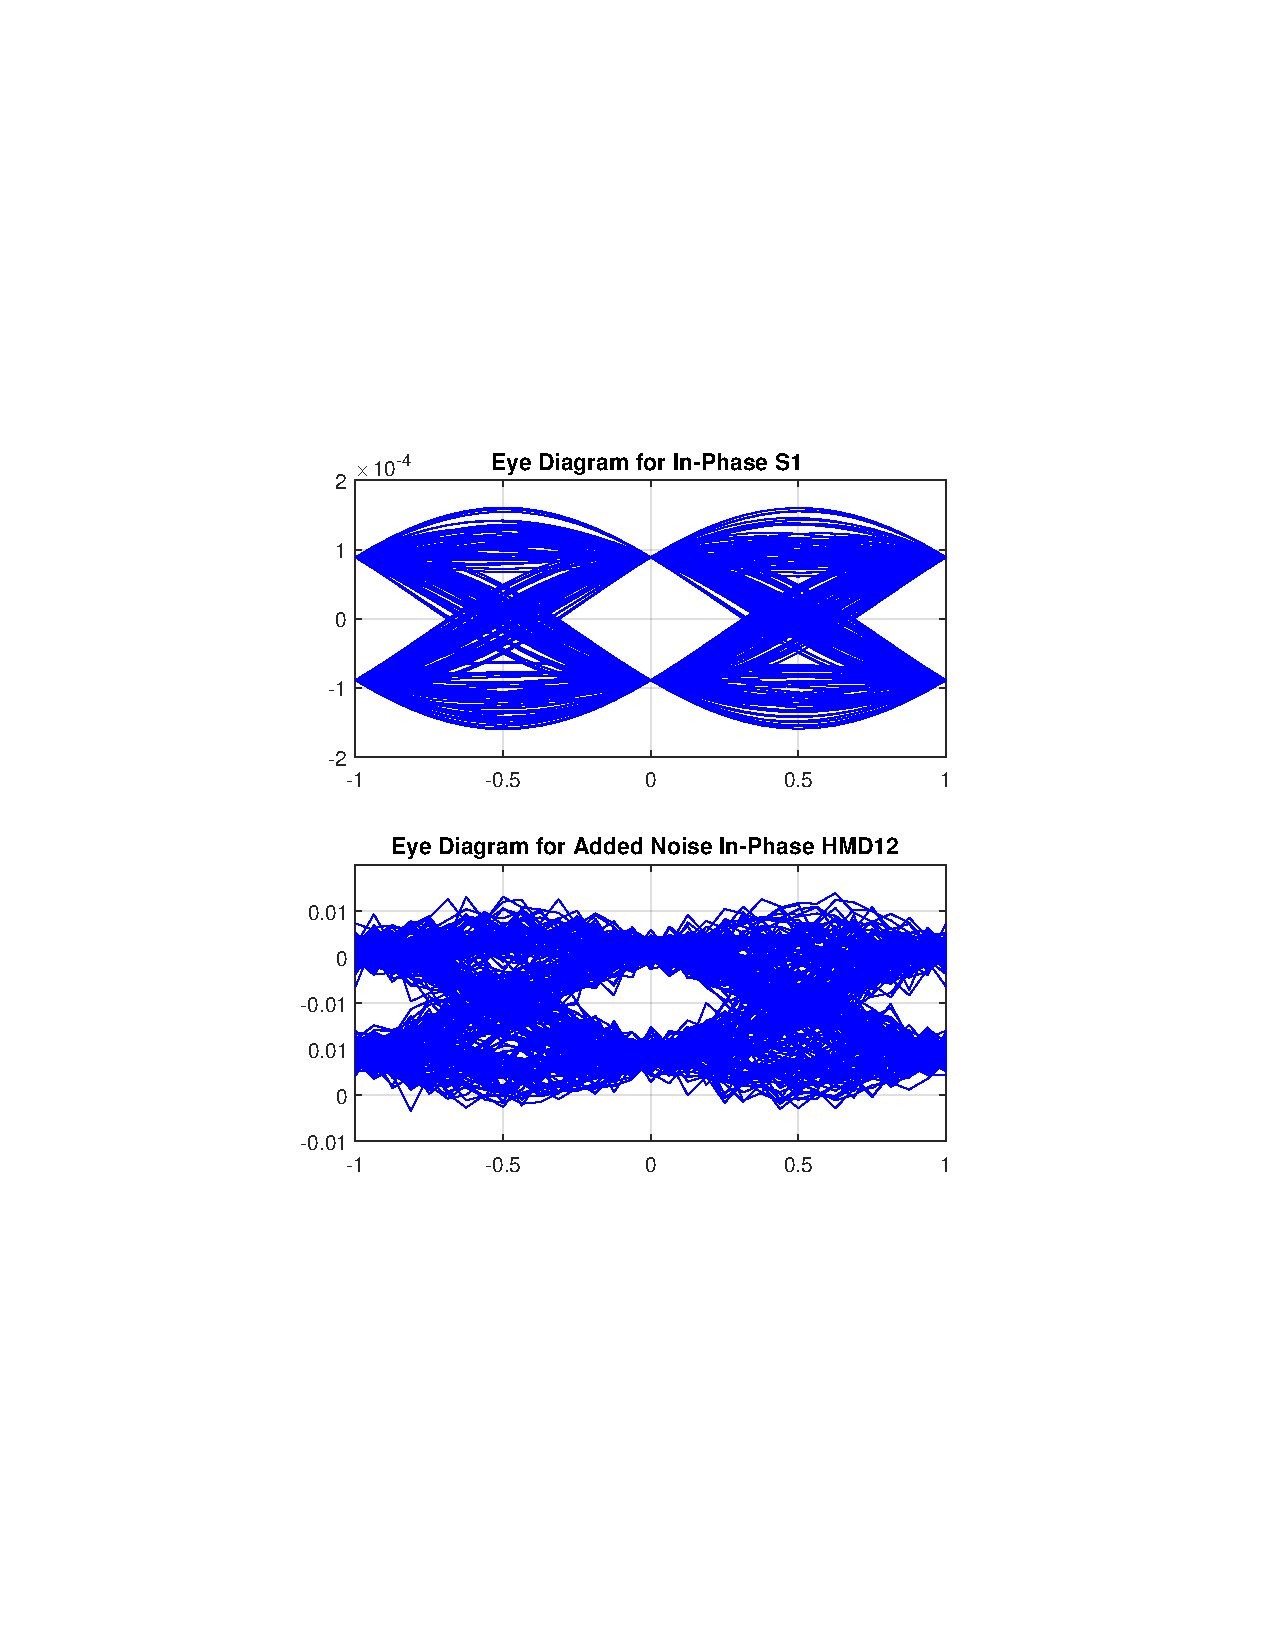
\includegraphics[clip, trim=5cm 7cm 5cm 7cm, width=\textwidth]{./sdf/m_qam_system/figures/eyes/if_n_nmf_45_60_rc.pdf}
	\end{subfigure}
	\begin{subfigure}{.45\textwidth}
		\centering
		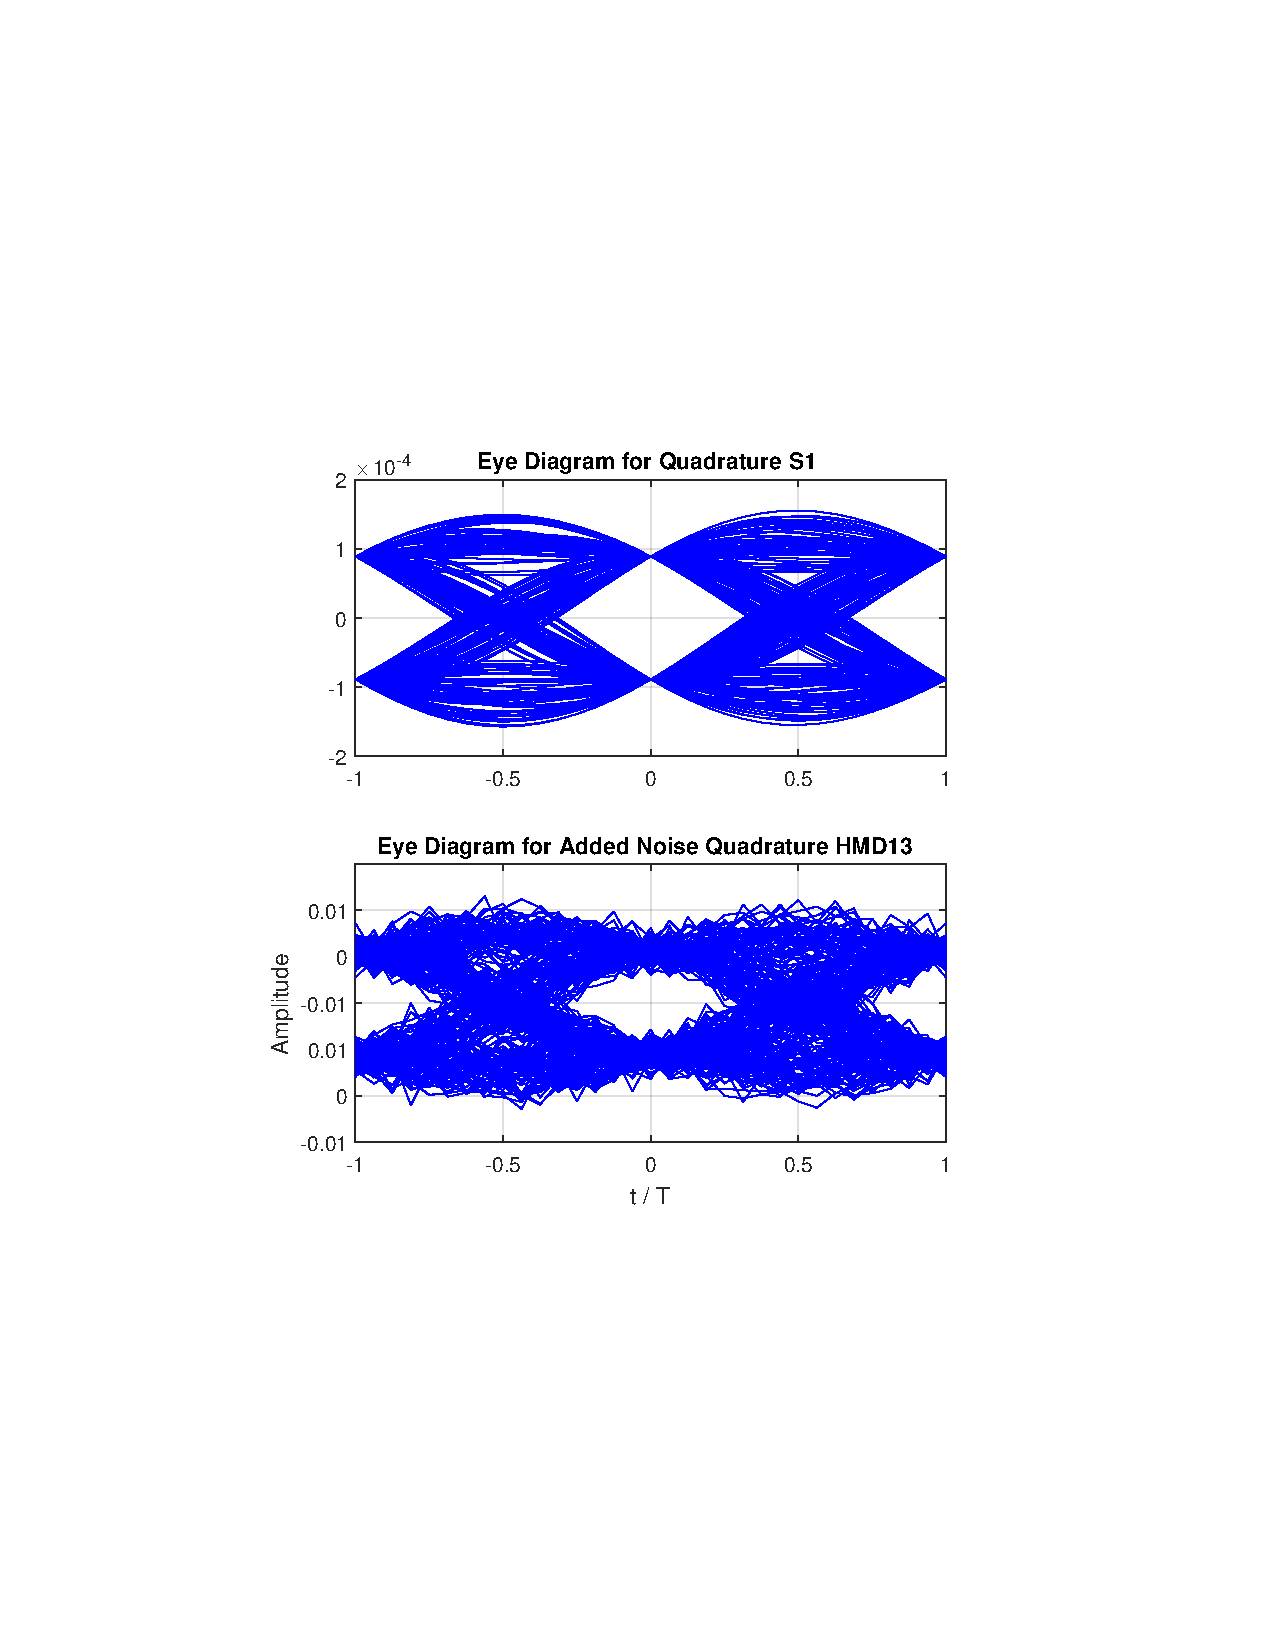
\includegraphics[clip, trim=5cm 7cm 5cm 7cm, width=\textwidth]{./sdf/m_qam_system/figures/eyes/q_n_nmf_45_60_rc.pdf}
	\end{subfigure}
	
	\caption{
%		Eye diagrams without matched filtering with raised-cosine.
		Obtained
		at two different points in the system: optical output of transmitter on the top and
		the noisy signal at the bottom.
%		Simulation done with an optical power output of
%		-45~dBm, 0~dBm at the local oscillator, a gain of $10^3$ at the amplifier, a
%		noise spectral density of $10^{-6}$ and a rolloff factor of
%		0.3.
		\label{fig:eyes_n_rc_45_03}}
	\end{minipage}
\end{figure}
\begin{table}[H]
	\centering
	\footnotesize
	\begin{tabular}{|l|l|}
		\hline
		\multicolumn{2}{|c|}{ \textbf{Simulation Parameters} } \\
		\hline
		\textbf{Parameter}     & \textbf{Default Value}                                     \\\hline
		%		numberOfBitsGenerated  & $40000$	                                                \\\hline
		bitPeriod              & $1/50\times10^9$~s														\\\hline
		%		symbolRate		       &                                                     		\\\hline
		samplesPerSymbol       & $16$                                                       \\\hline
		%		symbolRate		       &                                                     		\\\hline
		%		pLength                & $5$                                                        \\\hline
		%		iqAmplitudesValues     & $\lbrace~\lbrace-1,~0\rbrace~,~\lbrace1,~0\rbrace~\rbrace$ \\\hline
		outputOpticalPower     & $-45$~dBm 													\\ \hline
		shaperFilter	       & RootRaisedCosine												\\ \hline
		outputFilter		   & RootRaisedCosine												\\ \hline
		rollOffFactor		   & 0.3														\\ \hline
		localOscillatorPower   & $0$~dBm                                                    \\ \hline
		localOscillatorPhase   & $0$                                                        \\ \hline
		%		transferMatrix         & $\lbrace~\lbrace \frac{1}{\sqrt{2}},~\frac{1}{\sqrt{2}},~\frac{1}{\sqrt{2}},~\frac{-1}{\sqrt{2}} \rbrace~\rbrace$ & \\ \hline
		responsivity           & $1$                                                        \\ \hline
		amplification          & $10^3$                                                     \\ \hline
		noisePower   & $10^{-6}$~V$^2$                             					\\ \hline
		theoreticalSNR  	   & $15~dB$                             					\\ \hline
		numericalSNR 		     & $14.9696~dB$                             					\\ \hline
		numericalSNR Upper Bound (95\% confidence) & $15.006~dB$                             					\\ \hline
		numericalSNR Lower Bound (95\% confidence) & $14.9329~dB$                             					\\ \hline
		%		confidence             & $0.95$                                                     \\ \hline
		%		midReportSize          & $0$                                                        \\ \hline
	\end{tabular}
\end{table}
\begin{figure}[H]
		\centering
	\textbf{Root-Raised-Cosine Signal (roll-off=0.3) with Added Noise and Matched Filtering, SNR = 15 dB}
	\begin{minipage}{\linewidth}
		\centering
	\begin{subfigure}{.45\textwidth}
		\centering
		\includegraphics[clip, trim=5cm 4cm 5cm 4cm, width=\textwidth]{./sdf/m_qam_system/figures/eyes/if_p_45_03.pdf}
	\end{subfigure}
	\begin{subfigure}{.45\textwidth}
		\centering
		\includegraphics[clip, trim=5cm 4cm 5cm 4cm, width=\textwidth]{./sdf/m_qam_system/figures/eyes/q_p_45_03.pdf}
	\end{subfigure}
	
	\caption{
%		Eye diagrams using matched filtering with root-raised-cosine.
		Obtained at three different points in the system: optical output of transmitter on the top;
		the amplified signal at the middle; and
		after the receiver filter.
%		Obtained through simulation with an optical
%		power output of -45~dBm, 0~dBm at the local oscillator, a gain of $10^3$ at the
%		amplifier, a noise spectral density of $10^{-6}$ and a rolloff factor of
%		0.3.
		\label{fig:eyes_n_rrc_45_03}}
	\end{minipage}
\end{figure}



\subsubsection*{Signals with AWGN and low SNR}
Figures \ref{fig:eyes_n_rrc_60_03}-\ref{fig:eyes_n_rc_60_09} show eye
diagrams similar to the previous section, but with a lower optical power ($-60~dBm$),
comparable to the average noise power ($10^{-6} V^2$).



Figures~\ref{fig:eyes_n_rc_60_09} and~\ref{fig:eyes_n_rrc_60_09} show the
diagrams obtained without matched filtering and with matched filtering,
respectively, both using a roll-off factor of 0.9.

In this example the effects of matched filtering is even more obvious, as
without it the signal visually appears to be random noise.
\begin{table}[H]
	\centering
	\footnotesize
	\begin{tabular}{|l|l|}
		\hline
		\multicolumn{2}{|c|}{ \textbf{Simulation Parameters} } \\
		\hline
		\textbf{Parameter}     & \textbf{Default Value}                                     \\\hline
		%		numberOfBitsGenerated  & $40000$	                                                \\\hline
		bitPeriod              & $1/50\times10^9$~s														\\\hline
		%		symbolRate		       &                                                     		\\\hline
		samplesPerSymbol       & $16$                                                       \\\hline
		%		symbolRate		       &                                                     		\\\hline
		%		pLength                & $5$                                                        \\\hline
		%		iqAmplitudesValues     & $\lbrace~\lbrace-1,~0\rbrace~,~\lbrace1,~0\rbrace~\rbrace$ \\\hline
		outputOpticalPower     & $-60$~dBm 													\\ \hline
		shaperFilter	       & RaisedCosine												\\ \hline
		outputFilter		   &                											\\ \hline
		rollOffFactor		   & 0.9														\\ \hline
		localOscillatorPower   & $0$~dBm                                                    \\ \hline
		localOscillatorPhase   & $0$                                                        \\ \hline
		%		transferMatrix         & $\lbrace~\lbrace \frac{1}{\sqrt{2}},~\frac{1}{\sqrt{2}},~\frac{1}{\sqrt{2}},~\frac{-1}{\sqrt{2}} \rbrace~\rbrace$ & \\ \hline
		responsivity           & $1$                                                        \\ \hline
		amplification          & $10^3$                                                     \\ \hline
		noisePower   & $10^{-6}$~V$^2$                             					\\ \hline
		theoreticalSNR  	   & $0~dB$                             					\\ \hline
		numericalSNR 		     & $-1.07702~dB$                             					\\ \hline
		numericalSNR Upper Bound (95\% confidence) & $-1.0038~dB$                             					\\ \hline
		numericalSNR Lower Bound (95\% confidence) & $-1.1515~dB$                             					\\ \hline
		%		confidence             & $0.95$                                                     \\ \hline
		%		midReportSize          & $0$                                                        \\ \hline
	\end{tabular}
\end{table}
\begin{figure}[H]
		\centering
	\textbf{Raised-Cosine Signal (roll-off=0.9) with Added Noise, SNR = 0~dB}
	\begin{minipage}{\linewidth}
		\centering
	\begin{subfigure}{.45\textwidth}
		\centering
		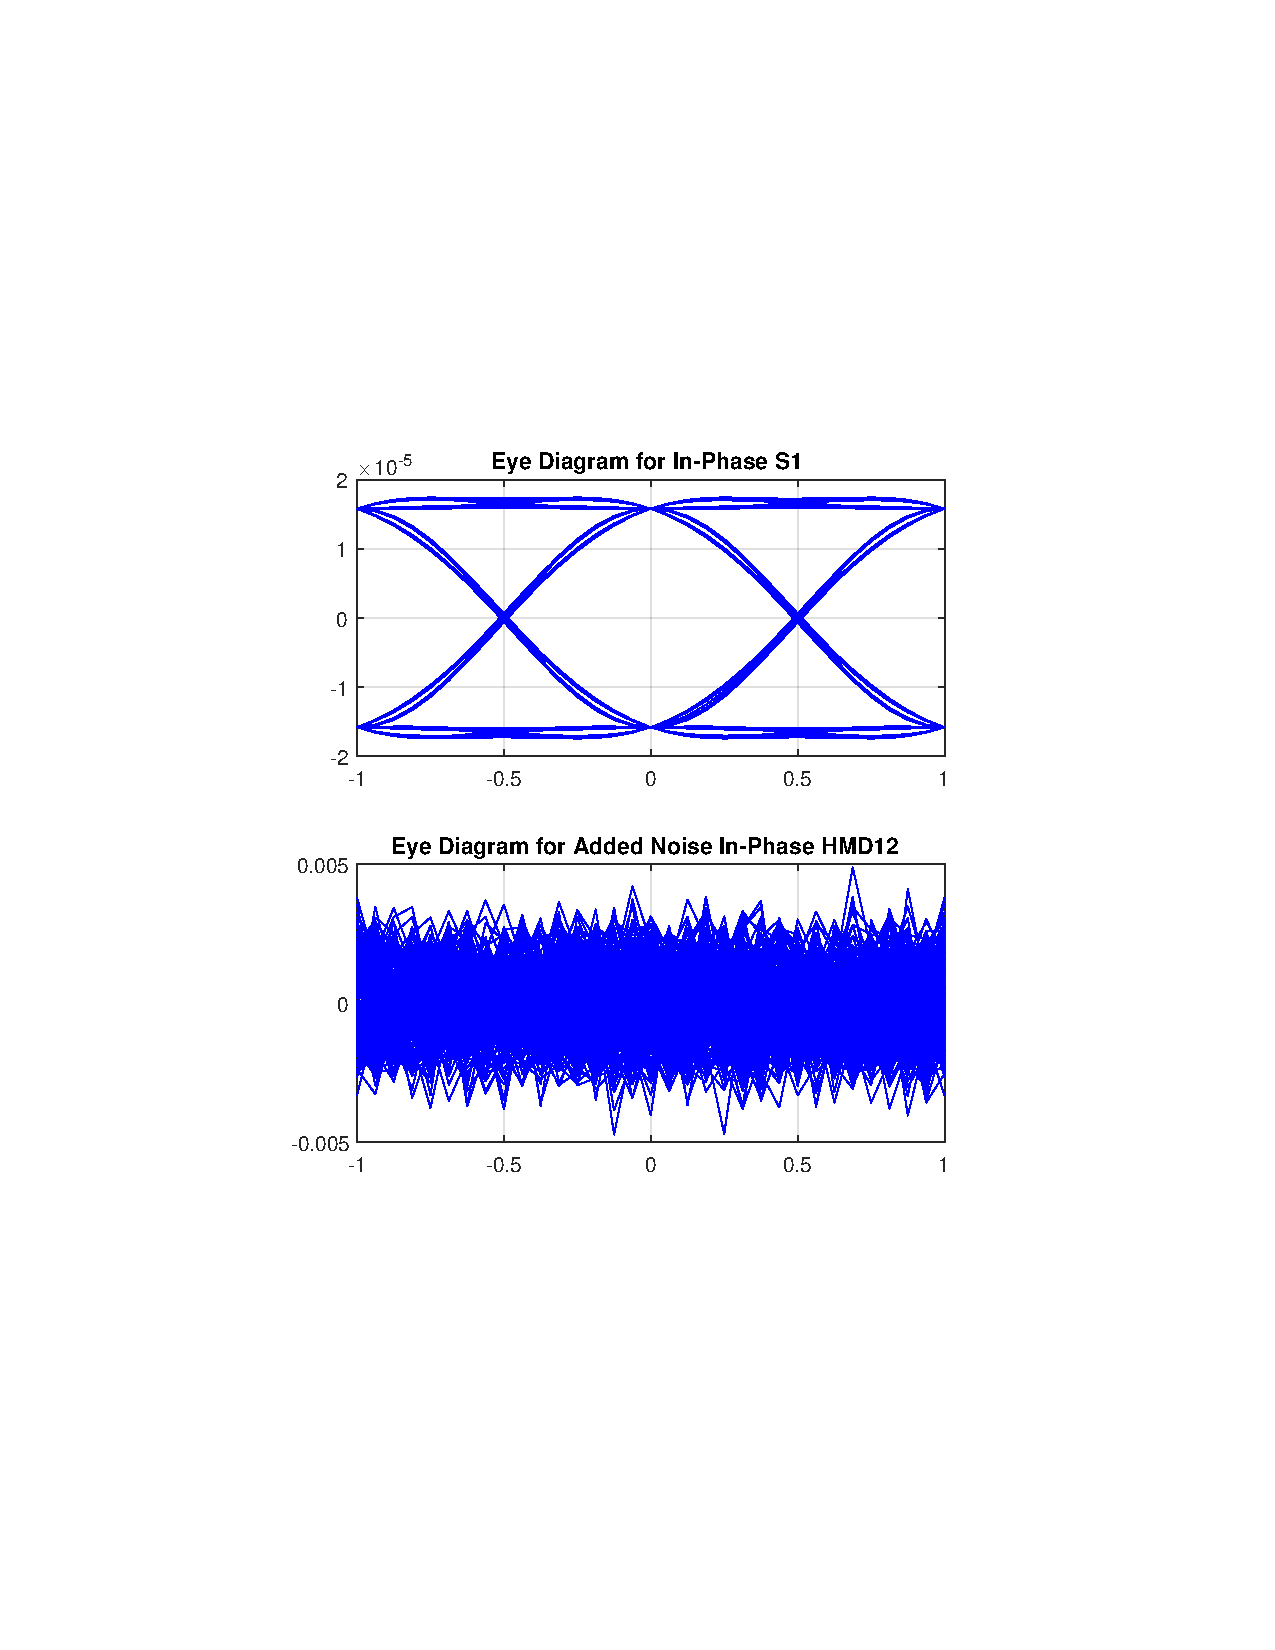
\includegraphics[clip, trim=5cm 7cm 5cm 7cm, width=\textwidth]{./sdf/m_qam_system/figures/eyes/if_n_nmf_60_60_rc_09.pdf}
	\end{subfigure}
	\begin{subfigure}{.45\textwidth}
		\centering
		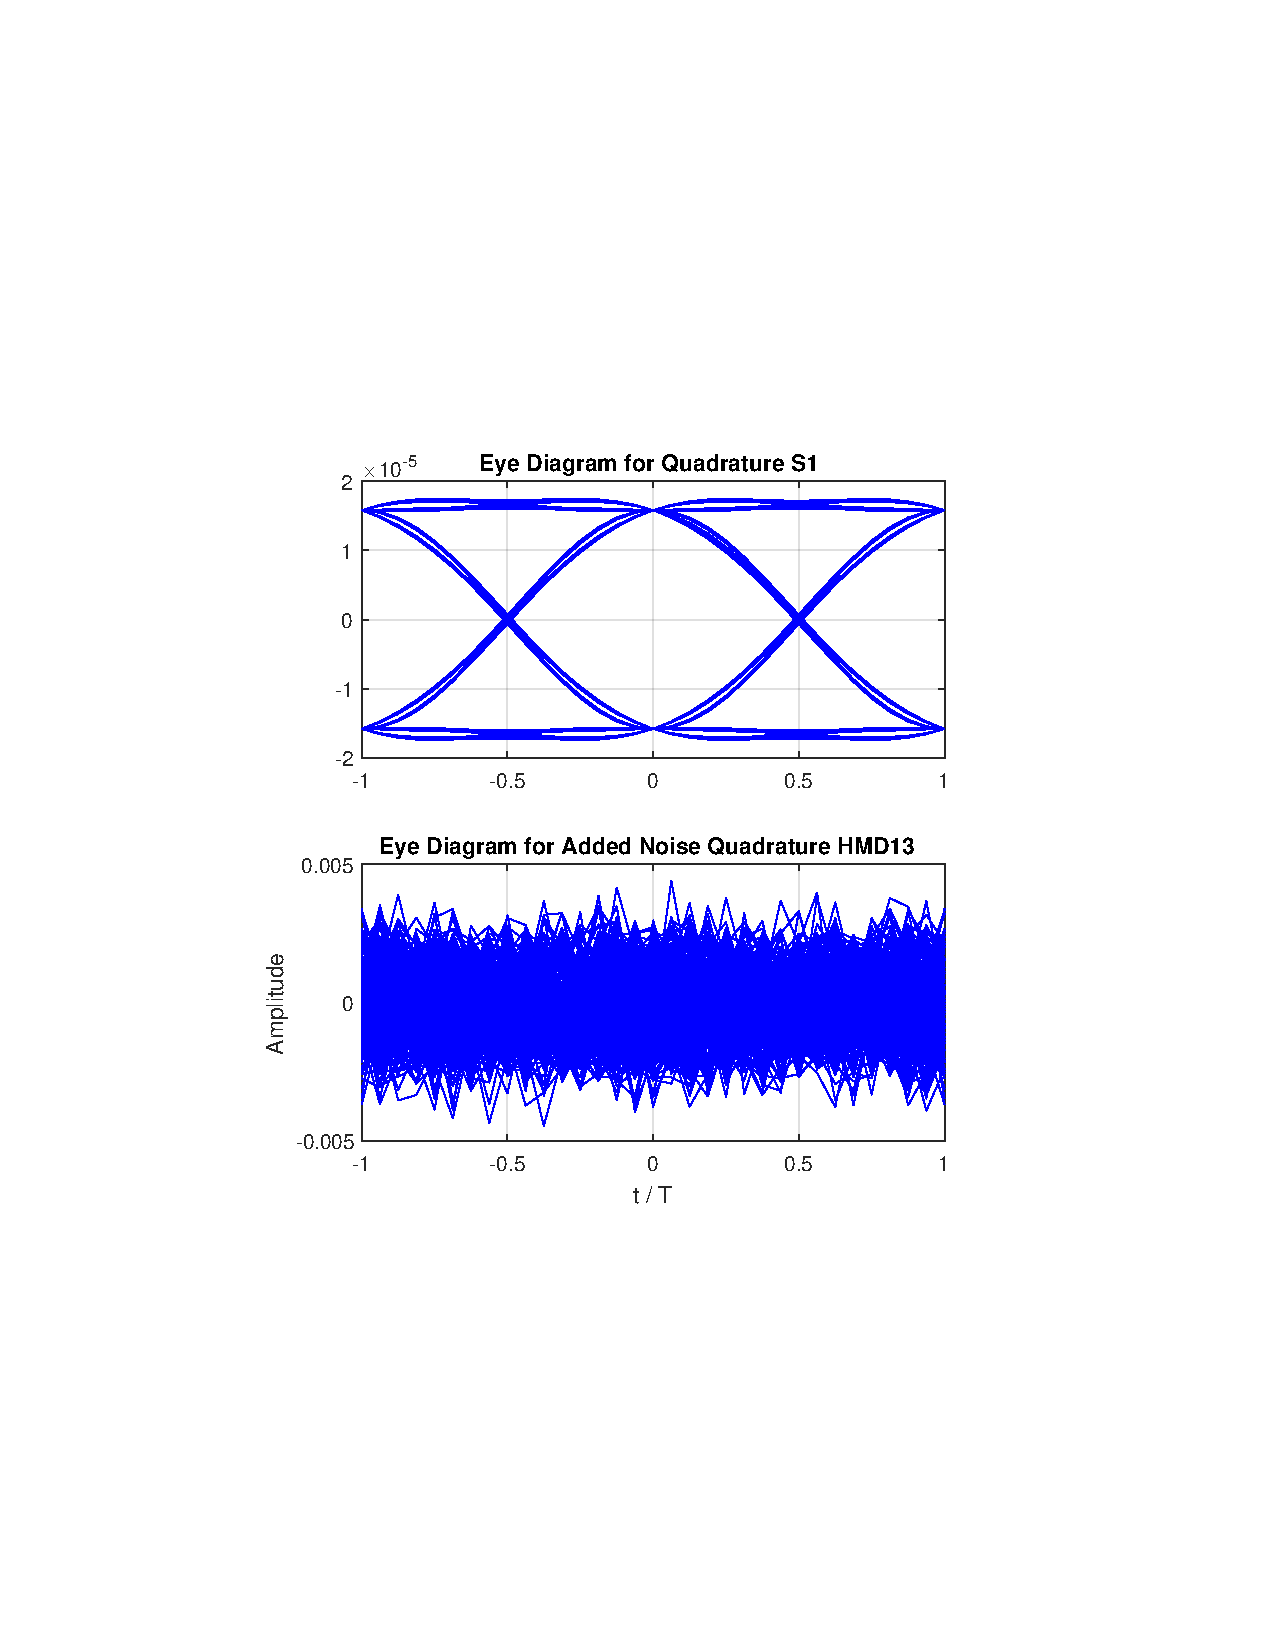
\includegraphics[clip, trim=5cm 7cm 5cm 7cm, width=\textwidth]{./sdf/m_qam_system/figures/eyes/q_n_nmf_60_60_rc_09.pdf}
	\end{subfigure}
	
	\caption{
%		Eye diagrams without matched filtering with raised-cosine.
		Obtained
		at two different points in the system: optical output of transmitter on the top and
		the noisy signal at the bottom.
%		Simulation done with an optical power output of -60~dBm,
%		0~dBm at the local oscillator, a gain of $10^3$ at the amplifier, a noise
%		spectral density of $10^{-6}$ and a rolloff factor of
%		0.9.
		\label{fig:eyes_n_rc_60_09}}
	\end{minipage}]
\end{figure}

\begin{table}[H]
	\centering
	\footnotesize
	\begin{tabular}{|l|l|}
		\hline
		\multicolumn{2}{|c|}{ \textbf{Simulation Parameters} } \\
		\hline
		\textbf{Parameter}     & \textbf{Default Value}                                     \\\hline
				%		numberOfBitsGenerated  & $40000$	                                                \\\hline
		bitPeriod              & $1/50\times10^9$~s														\\\hline
		%		symbolRate		       &                                                     		\\\hline
		samplesPerSymbol       & $16$                                                       \\\hline
		%		symbolRate		       &                                                     		\\\hline
		%		pLength                & $5$                                                        \\\hline
		%		iqAmplitudesValues     & $\lbrace~\lbrace-1,~0\rbrace~,~\lbrace1,~0\rbrace~\rbrace$ \\\hline
		outputOpticalPower     & $-60$~dBm 													\\ \hline
		shaperFilter	       & RootRaisedCosine												\\ \hline
		outputFilter		   & RootRaisedCosine												\\ \hline
		rollOffFactor		   & 0.9														\\ \hline
		localOscillatorPower   & $0$~dBm                                                    \\ \hline
		localOscillatorPhase   & $0$                                                        \\ \hline
		%		transferMatrix         & $\lbrace~\lbrace \frac{1}{\sqrt{2}},~\frac{1}{\sqrt{2}},~\frac{1}{\sqrt{2}},~\frac{-1}{\sqrt{2}} \rbrace~\rbrace$ & \\ \hline
		responsivity           & $1$                                                        \\ \hline
		amplification          & $10^3$                                                     \\ \hline
		noisePower   & $10^{-6}$~V$^2$                             					\\ \hline
				theoreticalSNR  	   & $0~dB$                             					\\ \hline
		numericalSNR 		     & $0.0290907~dB$                             					\\ \hline
		numericalSNR Upper Bound (95\% confidence) & $0.120973~dB$                             					\\ \hline
		numericalSNR Lower Bound (95\% confidence) & $-0.064778~dB$                             					\\ \hline
		%		confidence             & $0.95$                                                     \\ \hline
		%		midReportSize          & $0$                                                        \\ \hline
	\end{tabular}
\end{table}
\begin{figure}[H]
		\centering
	\textbf{Root-Raised-Cosine Signal (roll-off=0.9) with Added  and Matched Filtering, SNR = 0~dB}
	\begin{minipage}{\linewidth}
		\centering
	\begin{subfigure}{.45\textwidth}
		\centering
		\includegraphics[clip, trim=5cm 4cm 5cm 4cm, width=\textwidth]{./sdf/m_qam_system/figures/eyes/if_p_60_09.pdf}
	\end{subfigure}
	\begin{subfigure}{.45\textwidth}
		\centering
		\includegraphics[clip, trim=5cm 4cm 5cm 4cm, width=\textwidth]{./sdf/m_qam_system/figures/eyes/q_p_60_09.pdf}
	\end{subfigure}
	
	\caption{
%		Eye diagrams using matched filtering with root-raised-cosine.
		Obtained at three different points in the system: optical output of transmitter on the top;
		the amplified signal at the middle; and
		after the receiver filter.
%		Simulation done with an optical power output of -60~dBm, 0~dBm at the local oscillator, a gain of $10^3$ at the amplifier, a noise spectral density of $10^{-6}$ and a rolloff factor of 0.9.
		\label{fig:eyes_n_rrc_60_09}}
	\end{minipage}
\end{figure}


Figures~\ref{fig:eyes_n_rc_60_03} and~\ref{fig:eyes_n_rrc_60_09} show the same
case but using a roll-off factor of 0.3.
\begin{table}[H]
	\centering
	\footnotesize
	\begin{tabular}{|l|l|}
		\hline
		\multicolumn{2}{|c|}{ \textbf{Simulation Parameters} } \\
		\hline
		\textbf{Parameter}     & \textbf{Default Value}                                     \\\hline
		%		numberOfBitsGenerated  & $40000$	                                                \\\hline
		bitPeriod              & $1/50\times10^9$~s														\\\hline
		%		symbolRate		       &                                                     		\\\hline
		samplesPerSymbol       & $16$                                                       \\\hline
		%		symbolRate		       &                                                     		\\\hline
		%		pLength                & $5$                                                        \\\hline
		%		iqAmplitudesValues     & $\lbrace~\lbrace-1,~0\rbrace~,~\lbrace1,~0\rbrace~\rbrace$ \\\hline
		outputOpticalPower     & $-60$~dBm 													\\ \hline
		shaperFilter	       & RaisedCosine												\\ \hline
		outputFilter		   &   												\\ \hline
		rollOffFactor		   & 0.3														\\ \hline
		localOscillatorPower   & $0$~dBm                                                    \\ \hline
		localOscillatorPhase   & $0$                                                        \\ \hline
		%		transferMatrix         & $\lbrace~\lbrace \frac{1}{\sqrt{2}},~\frac{1}{\sqrt{2}},~\frac{1}{\sqrt{2}},~\frac{-1}{\sqrt{2}} \rbrace~\rbrace$ & \\ \hline
		responsivity           & $1$                                                        \\ \hline
		amplification          & $10^3$                                                     \\ \hline
		noisePower   & $10^{-6}$~V$^2$                             					\\ \hline
						theoreticalSNR  	   & $0~dB$                             					\\ \hline
		numericalSNR 		     & $-0.306456~dB$                             					\\ \hline
		numericalSNR Upper Bound (95\% confidence) & $-0.233164~dB$                             					\\ \hline
		numericalSNR Lower Bound (95\% confidence) & $-0.381006~dB$                             					\\ \hline
		%		confidence             & $0.95$                                                     \\ \hline
		%		midReportSize          & $0$                                                        \\ \hline
	\end{tabular}
\end{table}
\begin{figure}[H]
		\centering
	\textbf{Raised-Cosine Signal (roll-off=0.3) with Added Noise, SNR = 0~dB}
	\begin{minipage}{\linewidth}
		\centering
	\begin{subfigure}{.45\textwidth}
		\centering
		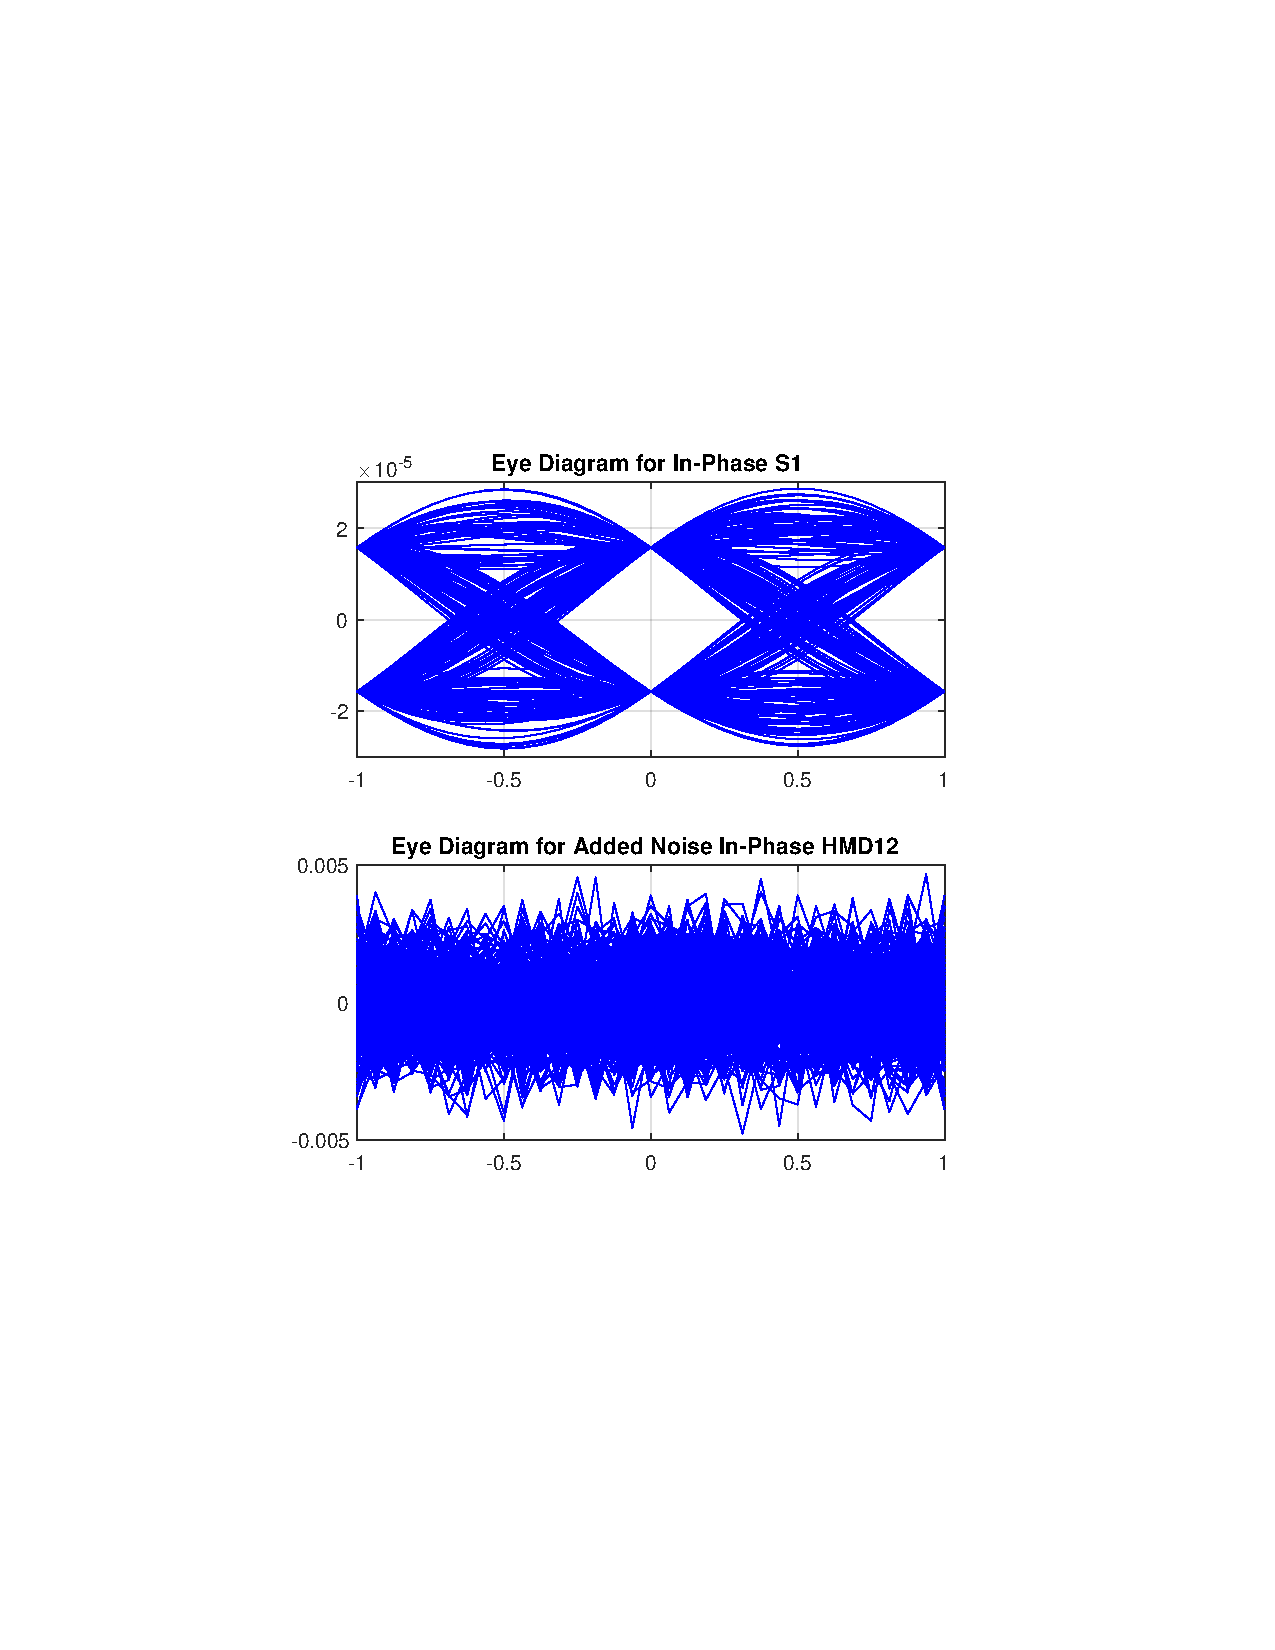
\includegraphics[clip, trim=5cm 7cm 5cm 7cm, width=\textwidth]{./sdf/m_qam_system/figures/eyes/if_n_nmf_60_60_rc_03.pdf}
	\end{subfigure}
	\begin{subfigure}{.45\textwidth}
		\centering
		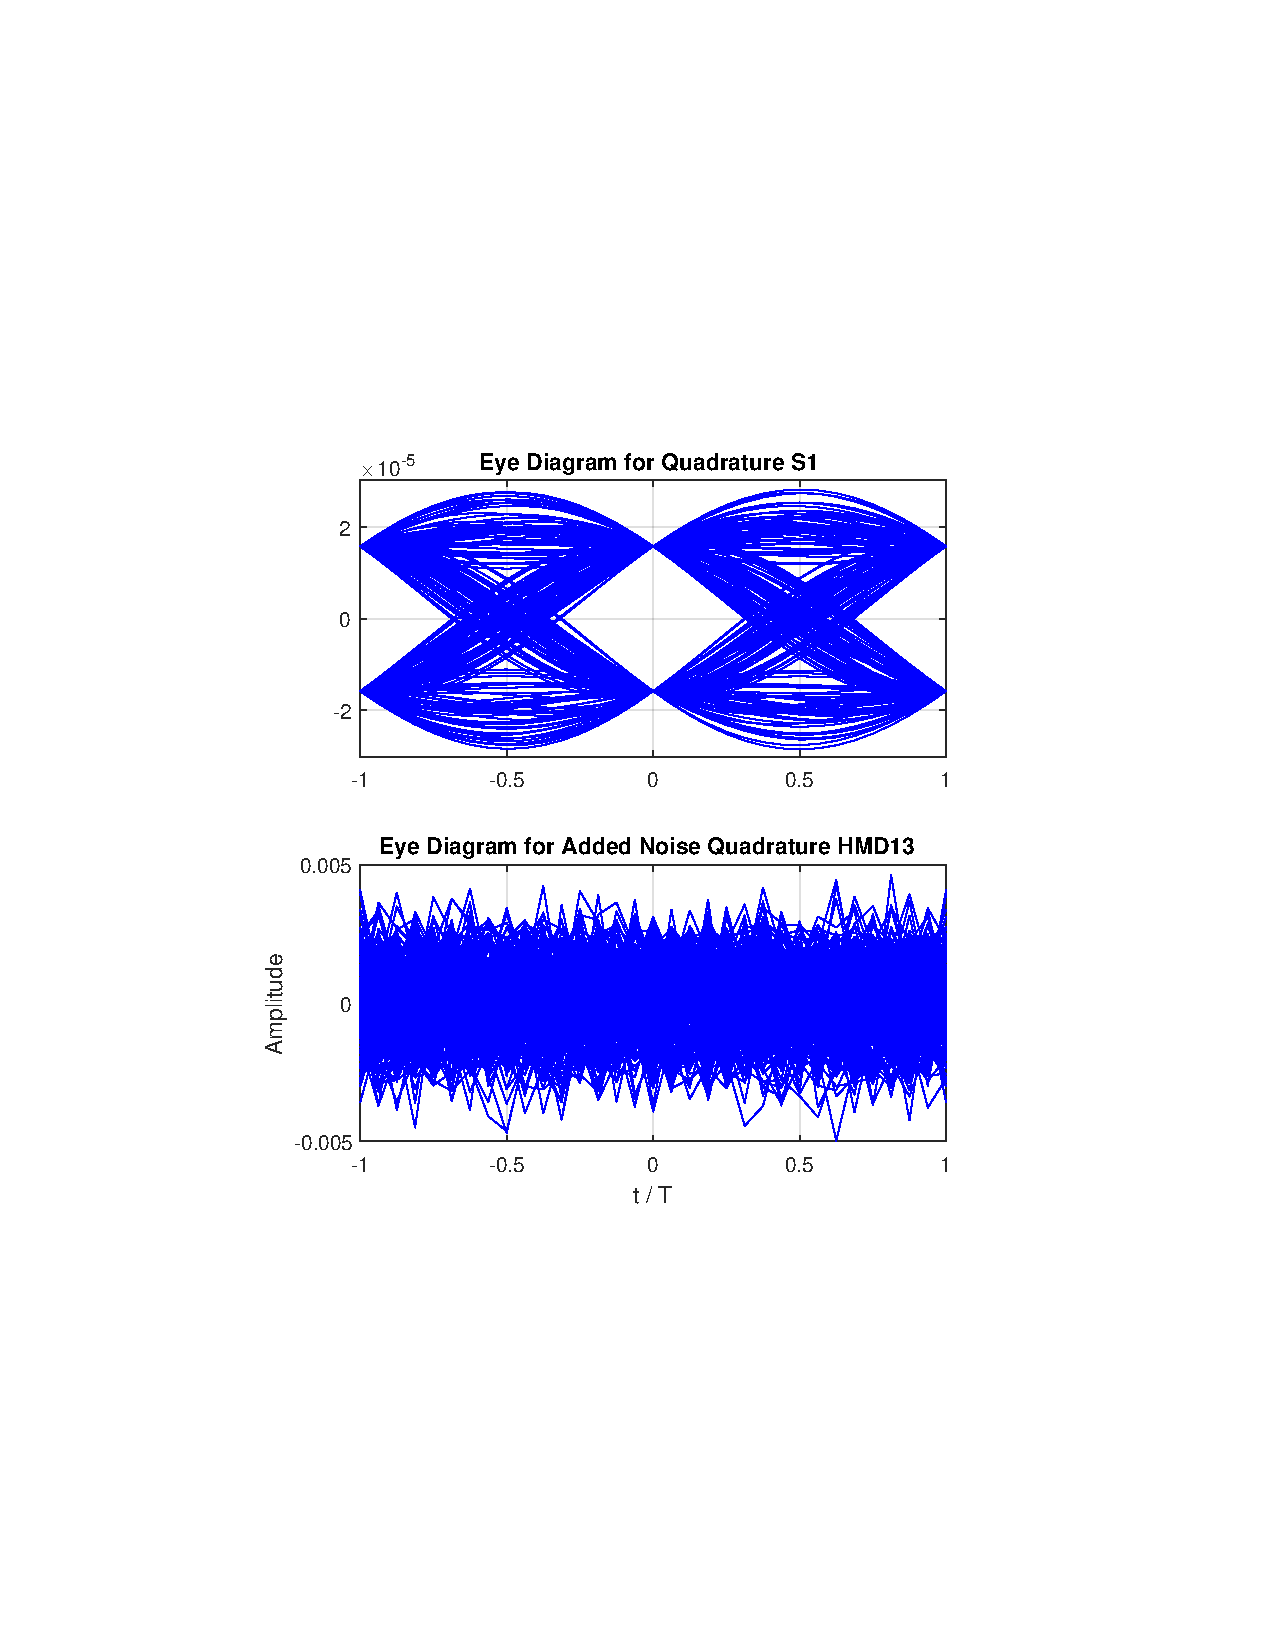
\includegraphics[clip, trim=5cm 7cm 5cm 7cm, width=\textwidth]{./sdf/m_qam_system/figures/eyes/q_n_nmf_60_60_rc_03.pdf}
	\end{subfigure}
	
	\caption{
%		Eye diagrams without matched-filtering with raised-cosine.
		Obtained
		at two different points in the system: optical output of transmitter on the top and
		the noisy signal at the bottom.
%		Simulation done with an optical power output of -60~dBm, 0~dBm at
%		the local oscillator, a gain of $10^3$ at the amplifier, a noise spectral
%		density of $10^{-6}$ and a rolloff factor of 0.3.
		\label{fig:eyes_n_rrc_60_03}}
	\end{minipage}
\end{figure}
\begin{table}[H]
	\centering
	\footnotesize
	\begin{tabular}{|l|l|}
		\hline
		\multicolumn{2}{|c|}{ \textbf{Simulation Parameters} } \\
		\hline
		\textbf{Parameter}     & \textbf{Default Value}                                     \\\hline
		%		numberOfBitsGenerated  & $40000$	                                                \\\hline
		bitPeriod              & $1/50\times10^9$~s														\\\hline
		%		symbolRate		       &                                                     		\\\hline
		samplesPerSymbol       & $16$                                                       \\\hline
		%		symbolRate		       &                                                     		\\\hline
		%		pLength                & $5$                                                        \\\hline
		%		iqAmplitudesValues     & $\lbrace~\lbrace-1,~0\rbrace~,~\lbrace1,~0\rbrace~\rbrace$ \\\hline
		outputOpticalPower     & $-60$~dBm 													\\ \hline
		shaperFilter	       & RootRaisedCosine												\\ \hline
		outputFilter		   & RootRaisedCosine												\\ \hline
		rollOffFactor		   & 0.3														\\ \hline
		localOscillatorPower   & $0$~dBm                                                    \\ \hline
		localOscillatorPhase   & $0$                                                        \\ \hline
		%		transferMatrix         & $\lbrace~\lbrace \frac{1}{\sqrt{2}},~\frac{1}{\sqrt{2}},~\frac{1}{\sqrt{2}},~\frac{-1}{\sqrt{2}} \rbrace~\rbrace$ & \\ \hline
		responsivity           & $1$                                                        \\ \hline
		amplification          & $10^3$                                                     \\ \hline
		noisePower   & $10^{-6}$~V$^2$                             					\\ \hline
								theoreticalSNR  	   & $0~dB$                             					\\ \hline
		numericalSNR 		     & $0.0368278~dB$                             					\\ \hline
		numericalSNR Upper Bound (95\% confidence) & $0.09153~dB$                             					\\ \hline
		numericalSNR Lower Bound (95\% confidence) & $-0.0185722~dB$                             					\\ \hline
		%		confidence             & $0.95$                                                     \\ \hline
		%		midReportSize          & $0$                                                        \\ \hline
	\end{tabular}
\end{table}
\begin{figure}[H]
		\centering
	\textbf{Root-Raised-Cosine Signal (roll-off=0.3) with Added Noise and Matched Filtering,\\ SNR = 0~dB}
	\begin{minipage}{\linewidth}
		\centering
	\begin{subfigure}{.45\textwidth}
		\centering
		\includegraphics[clip, trim=5cm 4cm 5cm 4cm, width=\textwidth]{./sdf/m_qam_system/figures/eyes/if_p_60_03.pdf}
	\end{subfigure}
	\begin{subfigure}{.45\textwidth}
		\centering
		\includegraphics[clip, trim=5cm 4cm 5cm 4cm, width=\textwidth]{./sdf/m_qam_system/figures/eyes/q_p_60_03.pdf}
	\end{subfigure}
	
	\caption{
%		Eye diagrams using matched filtering with root-raised-cosine.
		Obtained at three different points in the system: optical output of transmitter on the top;
		the amplified signal at the middle; and
		after the receiver filter.
%		Simulation done with an optical
%		power output of -60~dBm, 0~dBm at the local oscillator, a gain of $10^3$ at the
%		amplifier, a noise spectral density of $10^{-6}$ and a rolloff factor of
%		0.3.
		\label{fig:eyes_n_rc_60_03}}
	\end{minipage}
\end{figure}



\subsection*{BER Curves}

The simulated results show agreement with the theoretical curves, as can be seen in Figure~\ref{fig:ber_pseudorandom}.

\begin{table}[H]
	\centering
	\begin{tabular}{|l|l|}
	\hline
	\multicolumn{2}{|c|}{ \textbf{Simulation and Curve Parameters} } \\
		\hline
		\textbf{Parameter}     & \textbf{Default Value}                                     \\\hline
		numberOfBitsGenerated  & $40000$	                                                \\\hline
		samplingRate           & 64 GHz															\\\hline
		symbolRate		       & 4 GHz                                                    		\\\hline
		shaperFilter		   & Red Curve: RootRaisedCosine; Blue Curve: RaisedCosine	    \\\hline
		receiverFilter		   & Red Curve: RootRaisedCosine; Blue Curve: no filter 		\\\hline
		rollOff				   & 0.3														\\\hline
		%		samplesPerSymbol       & $16$                                                       \\\hline
		%		pLength                & $5$                                                        \\\hline
		%		iqAmplitudesValues     & $\lbrace~\lbrace-1,~0\rbrace~,~\lbrace1,~0\rbrace~\rbrace$ \\\hline
		outputOpticalPower     & Variable                                                   \\ \hline
		localOscillatorPower   & $0$~dBm                                                    \\ \hline
		%		localOscillatorPhase   & $0$                                                        \\ \hline
		%		transferMatrix         & $\lbrace~\lbrace	 \frac{1}{\sqrt{2}},~\frac{1}{\sqrt{2}},~\frac{1}{\sqrt{2}},~\frac{-1}{\sqrt{2}} \rbrace~\rbrace$ & \\ \hline
		responsivity           & $1$                                                        \\ \hline
		amplification          & $10^3$                                                     \\ \hline
		noisePower			   & $10^{-6}$~V$^2$                             					\\ \hline
		confidence             & $0.95$                                                     \\ \hline
		%			midReportSize          & $0$                                                        \\ \hline
	\end{tabular}
	\caption{Parameters for the theoretical curves and simulation results shown in Figure~\ref{fig:ber_pseudorandom}.\label{tab:ber_pseudorandom}}
\end{table}

\begin{figure}[H]
	\centering
		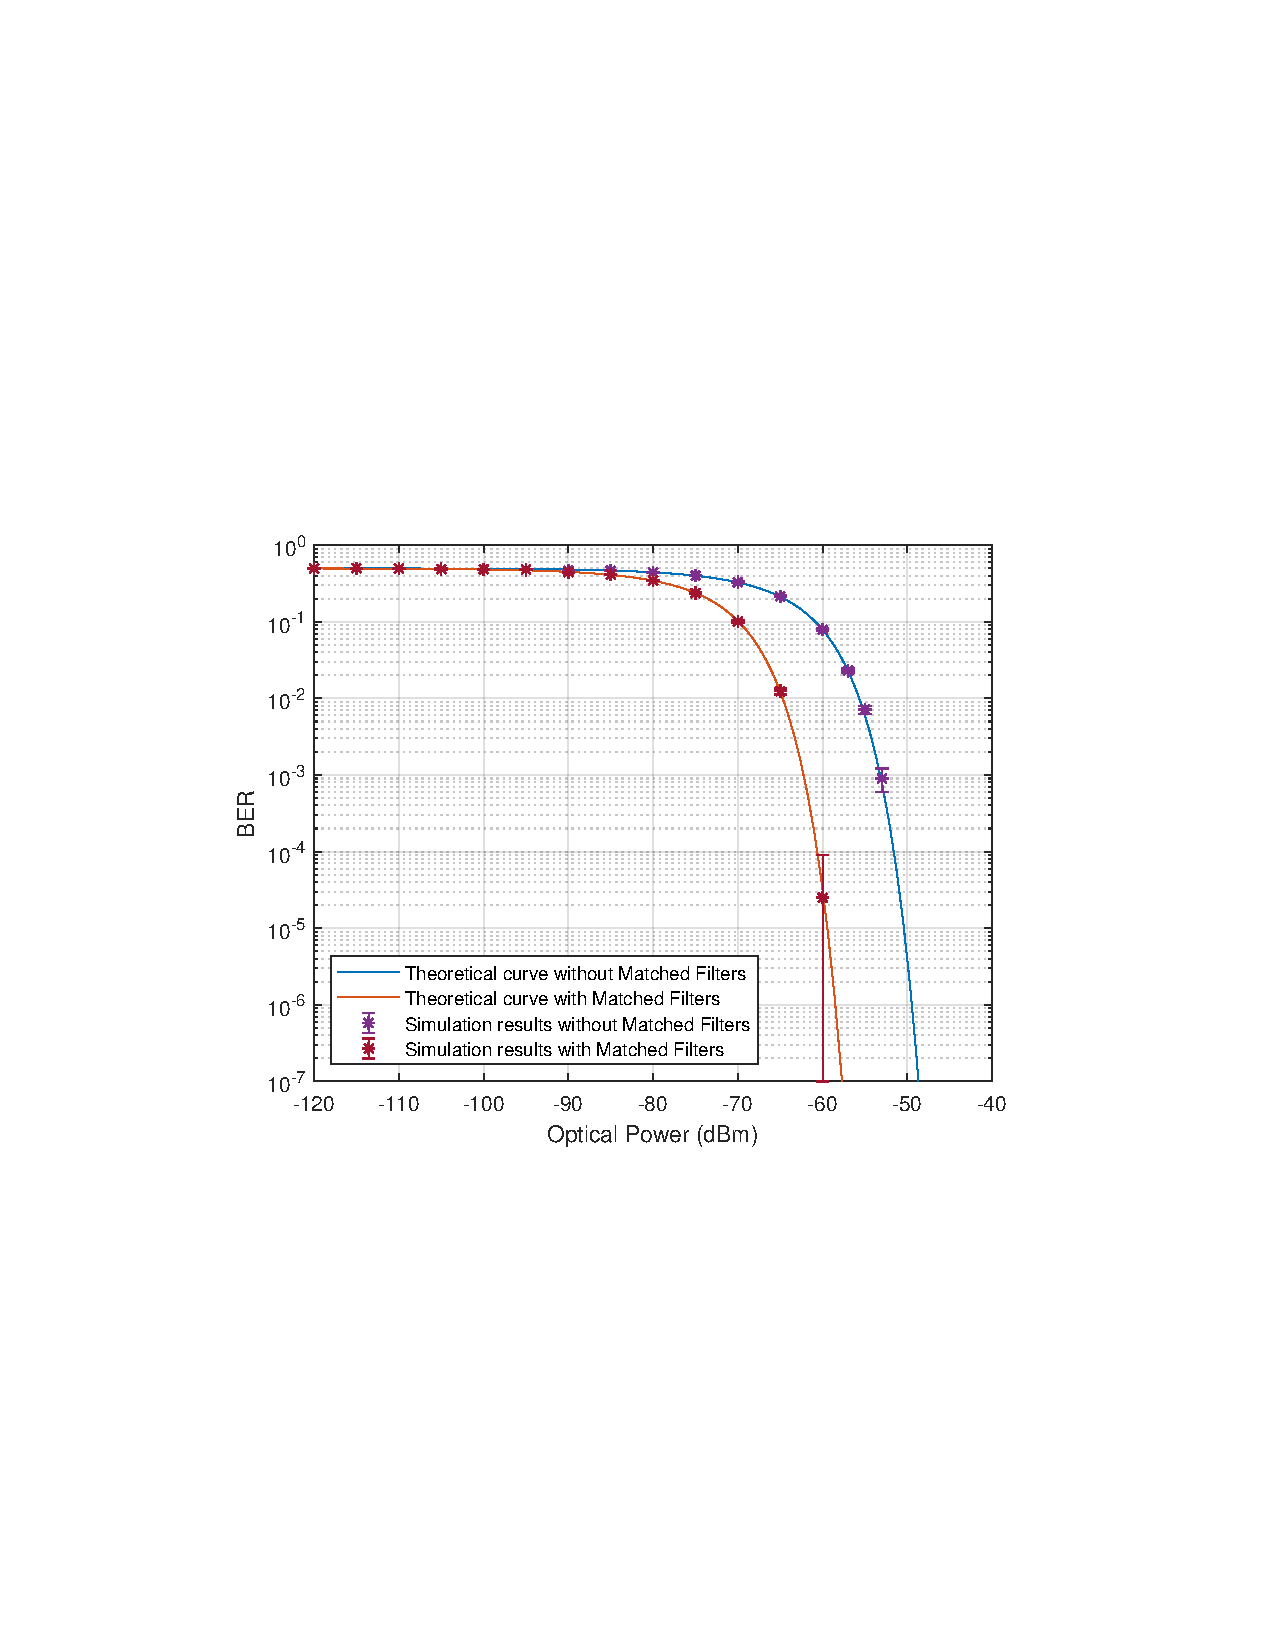
\includegraphics[clip, trim=4cm 8cm 4cm 8cm, width=0.7\textwidth]{./sdf/m_qam_system/figures/teor_vs_simul.pdf}
	%			
\caption{QPSK theoretical BER values as a function of the output optical power in dBm.\label{fig:ber_pseudorandom}}
\end{figure}

%\subsection*{Comparative Analysis}

In this section we show the simulation results and compared them with the theoretical predictions for an M-QAM system with $M=4$. Figure \ref{fig:ber_pseudorandom} shows the variation of the BER with the optical power of the signal, using $40000$ bits produced by a random number generator. The noise power was set at $10^{-6}~V^2$, the local oscillator at $0~dBm$ and the amplification at the transimpedance amplifier was set at $10^3$.
The red and blue lines represents the theoretical curve, with and without matched filters, respectively. The the red and purple points represent the simulated values for the same situation with the respective confidence margins. The simulation agrees closely with the theoretical values.



%\begin{figure}[h]
%	\centering
%	\includegraphics[clip, trim=4cm 8cm 4cm 8cm, width=0.7\textwidth]{./sdf/m_qam_system/figures/BER_QPSK_sim_mf_20180205.pdf}
%	\caption{Simulation result using root-raised cosine matched filtering for a random binary sequence with $40000$ bits, a noise power of $10^{-6}$ and an amplification of $10^3$.}
%	\label{fig:ber_pseudorandom_mf}
%\end{figure}%


%\begin{figure}[H]
%	\centering
%	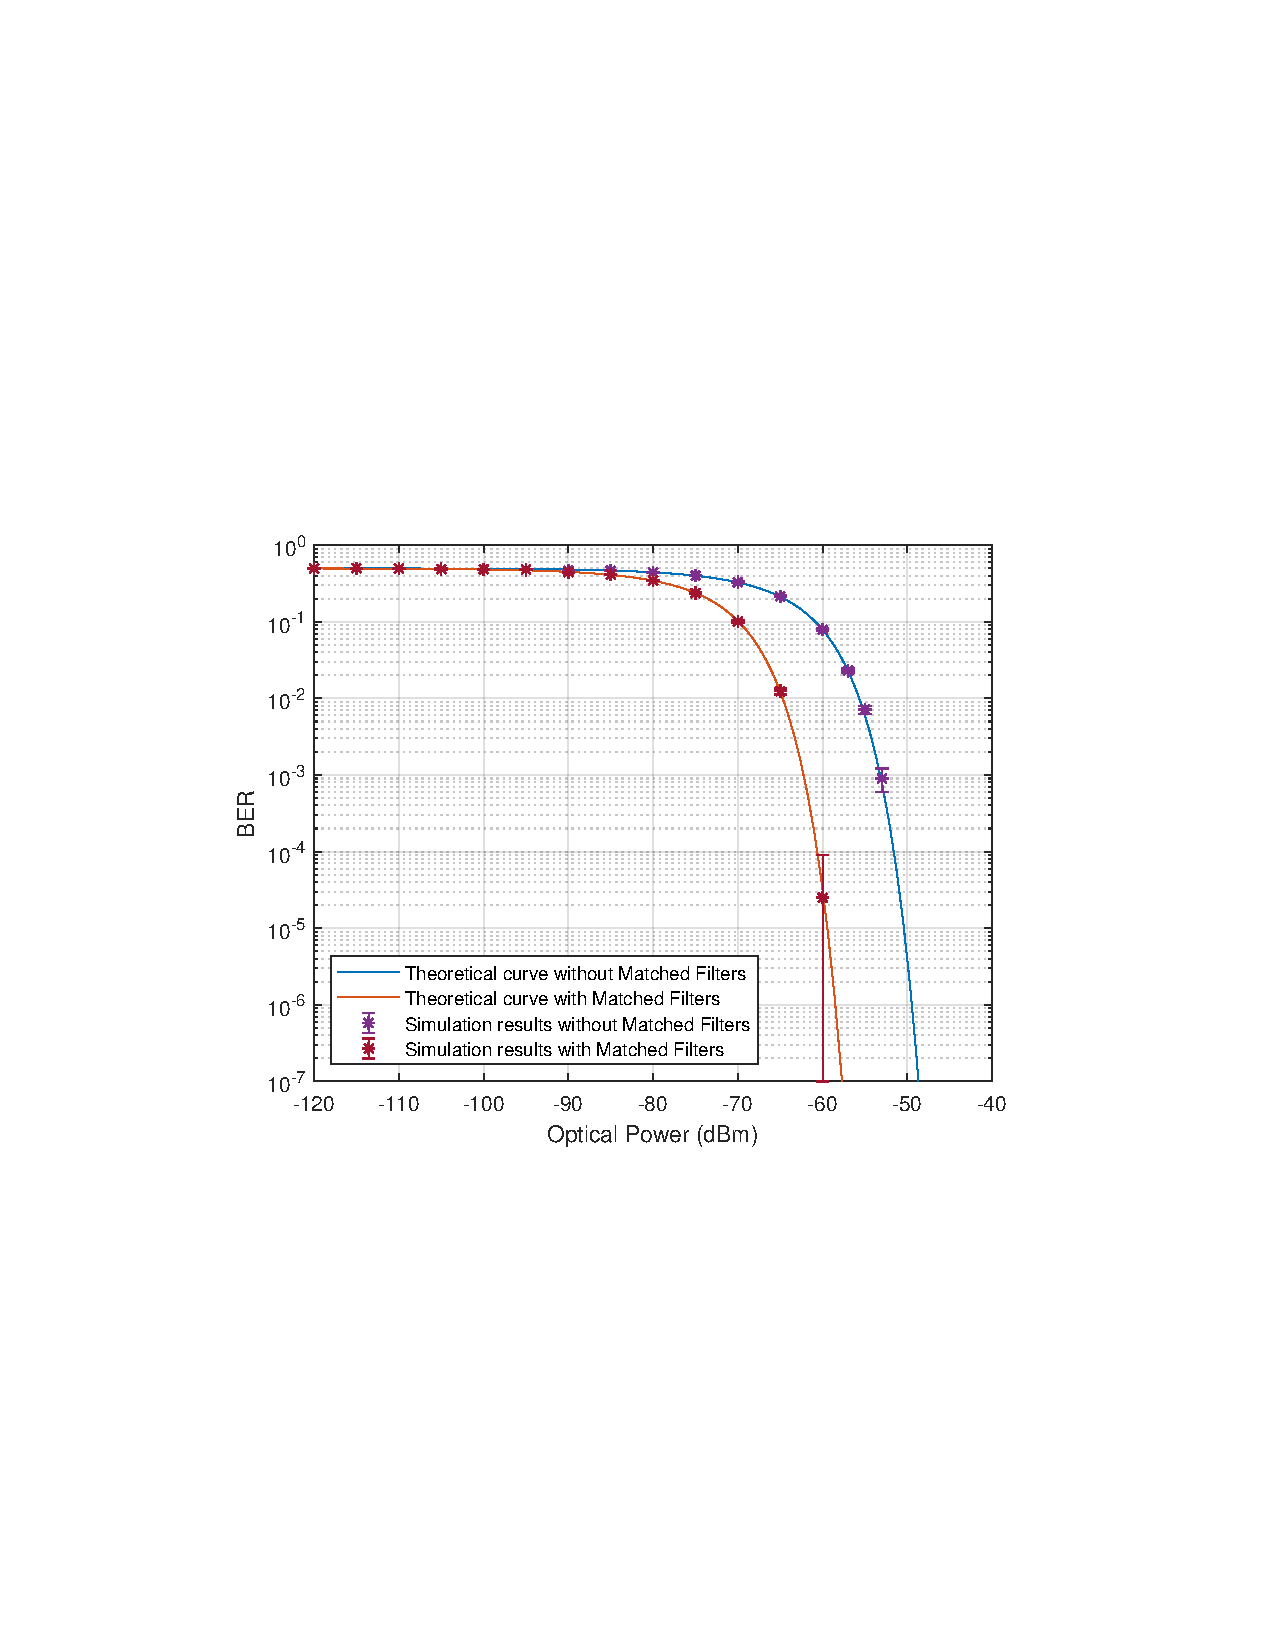
\includegraphics[clip, trim=4cm 8cm 4cm 8cm, width=0.7\textwidth]{./sdf/m_qam_system/figures/teor_vs_simul.pdf}
%	\caption{Simulation results for a random binary sequence with $40000$ bits, a noise power of $10^{-6}$ and an amplification of $10^3$. The simulated values which used a matched filter were obtained by shaping the pulse with a root-raised-cosine FIR filter and filtering the signal before the sample with the same filter. The results without matched filtering were obtained by using shaping the pulses with a raised-cosine filter. The margins shown were obtained for a 95\% confidence level.}
%\end{figure}%

\subsubsection*{Conclusions}
The use of a root-raised-cosine filters for shaping and filtering the signal provides the best results, due to reducing noise while creating no inter-symbol interference. The experimental BER curves agree with the theoretical values and show the advantages of matched filtering.

\subsection{Experimental Analysis}
\begin{figure}[H]
	\centering
	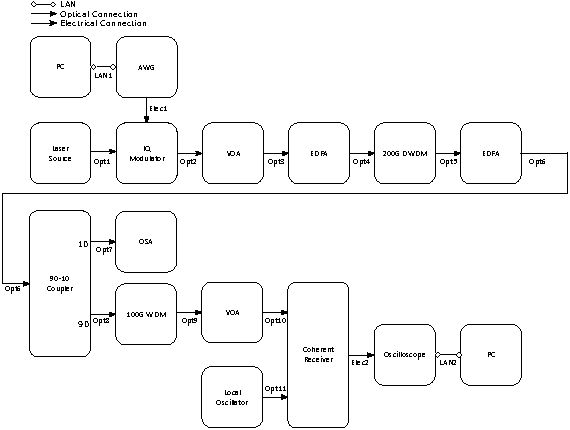
\includegraphics[width=\textwidth]{./sdf/m_qam_system/figures/mqamExperimental20180321.pdf}
	\caption{Experimental setup}
	\label{fig:experimental_mqam_setup}
\end{figure}

The setup shown in Figure~\ref{fig:experimental_mqam_setup} was used to obtain experimental results to compare with the theory and validate the simulation. The list of devices used for the setup is available in Table~\ref{tab:mqamdevices}.


%
%
\begin{table}[H]
	\centering
	\begin{tabulary}{1.0\textwidth}{|L|L|l|}
		\hline
		\textbf{Device}		& \textbf{Model}					& \textbf{Description}\\\hline
		Laser Source		& Yenista OSICS Band C/AG TLS Laser			& Optical laser source for modulate the signal \\\hline
		IQ Modulator 		& 22.5GHz IQ Modulator with automatic Bias Controller 	& \\\hline
		AWG 			& Keysight M8195A 					& \\\hline
		VOA			& 							& USB-Controlled Variable Optical Attenuator \\\hline
		EDFA			& Constelex Hydra-C-17-17 EDFA				& \\\hline
		200G DWDM		& 							& \\\hline
		EDFA			& Constelex Hydra-C-17-17 EDFA				& \\\hline
		90/10 Coupler		& 							& \\\hline
		OSA			& Apex Technologies AP-2043B 				& \\\hline
		100G WDM		& 							& \\\hline
		VOA			&							& \\\hline
		Local Oscillator	& Emcore CRTND3U02D ECL Laser				& \\\hline
		Coherent Receiver	& Picometrix CR-100D 					& \\\hline
		Oscilloscope		& Tektronix DPO77002SX-R3				& \\\hline
	\end{tabulary}
	\caption{Devices in experimental setup.~\label{tab:mqamdevices}}
\end{table}


Figure~\ref{fig:qamTxSig} to~\ref{fig:rxFinal} show the waveforms of the signal and the constellations at different points during the course of processing the received signal. All the waveforms shown correspond to the first 3 nanoseconds of the signal. The constellations assume that the signal has been sampled at the appropriate times unless otherwise noted.

Figure~\ref{fig:qamTxSig} shows the beginning of the signal generated by the AWG that was then sent to the IQ modulator.
The beginning of the signal received at the oscilloscope is shown in Figure~\ref{fig:qamRxSig}. Its worth noting that they are not synchronized, requiring that to be accomplished while processing after the aquisition. 

\begin{figure}[H]
	\centering
	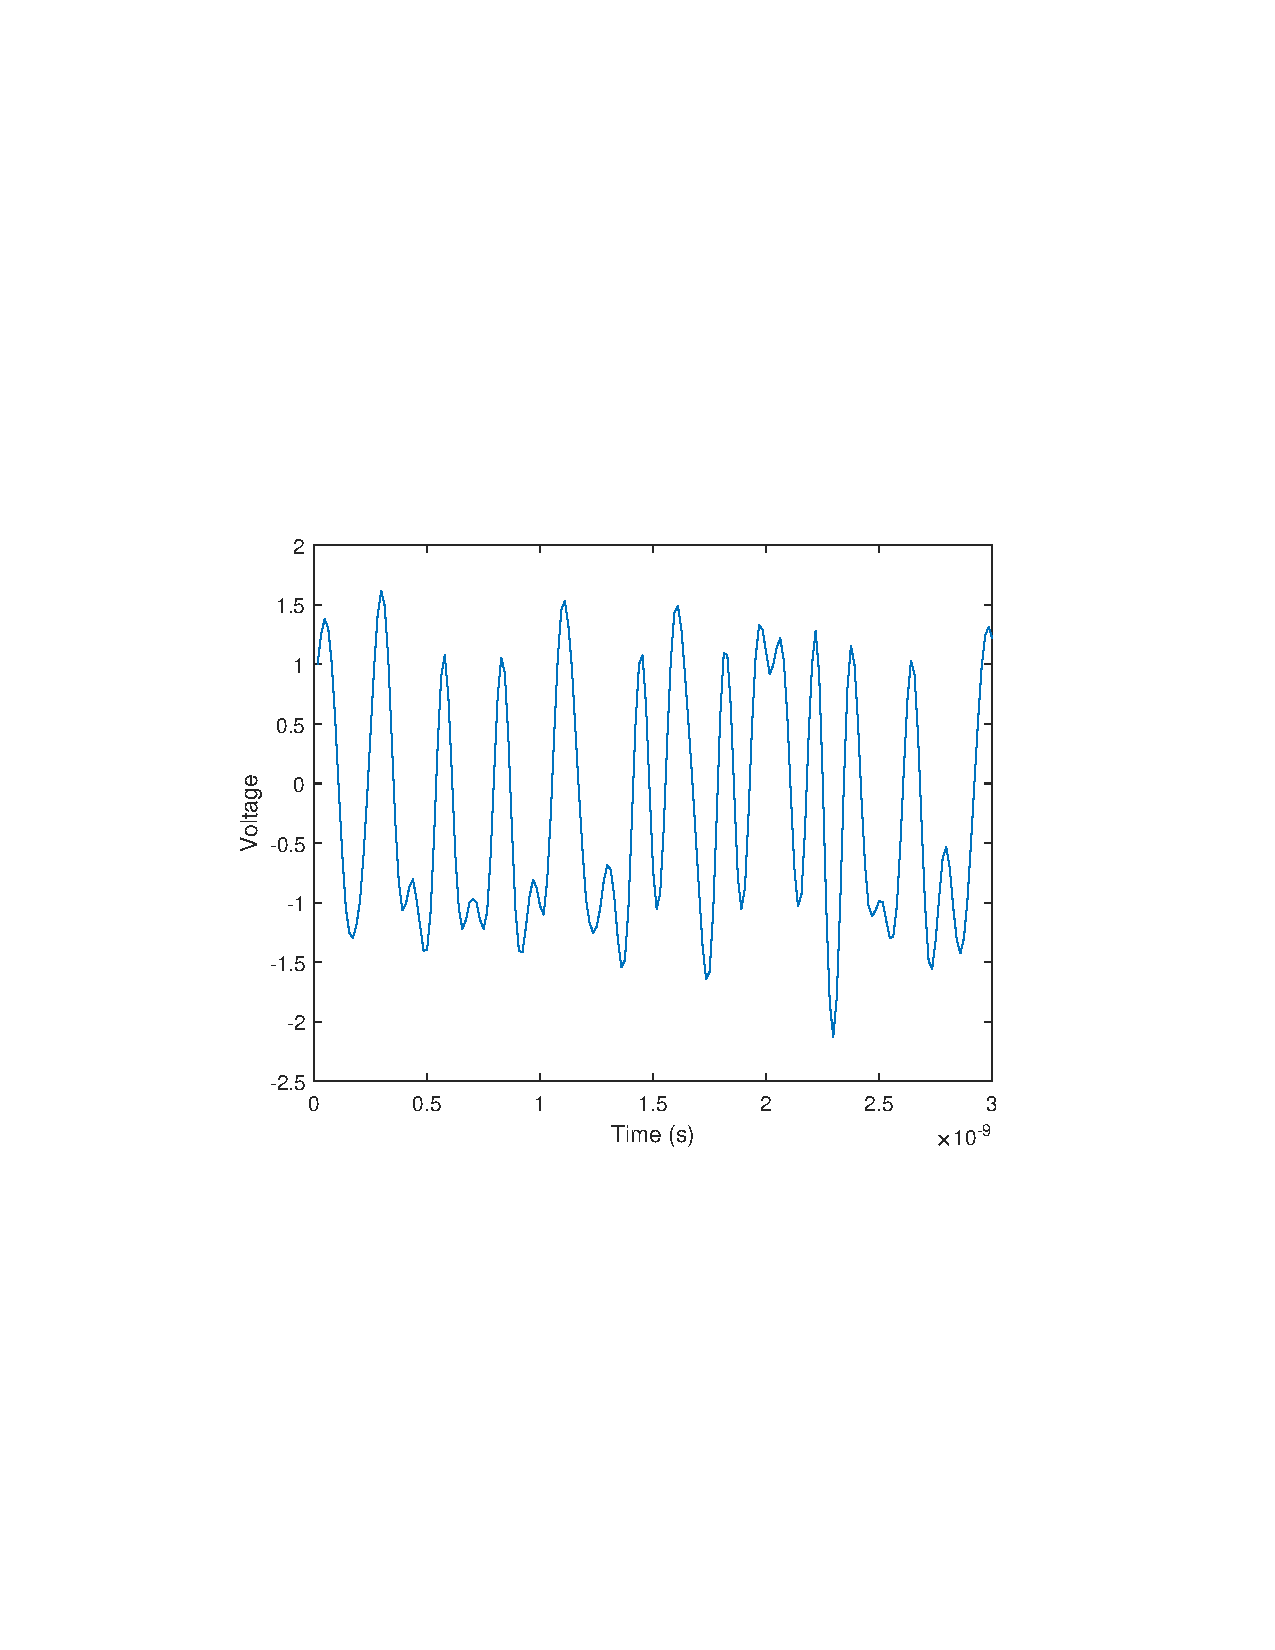
\includegraphics[clip, trim=4cm 8cm 4cm 8cm, width=0.7\textwidth]{./sdf/m_qam_system/figures/exp/TX_03.pdf}
	\caption{Signal sent to the IQ Modulator (Elec1).}
	\label{fig:qamTxSig}
\end{figure}

\begin{figure}[H]
\centering
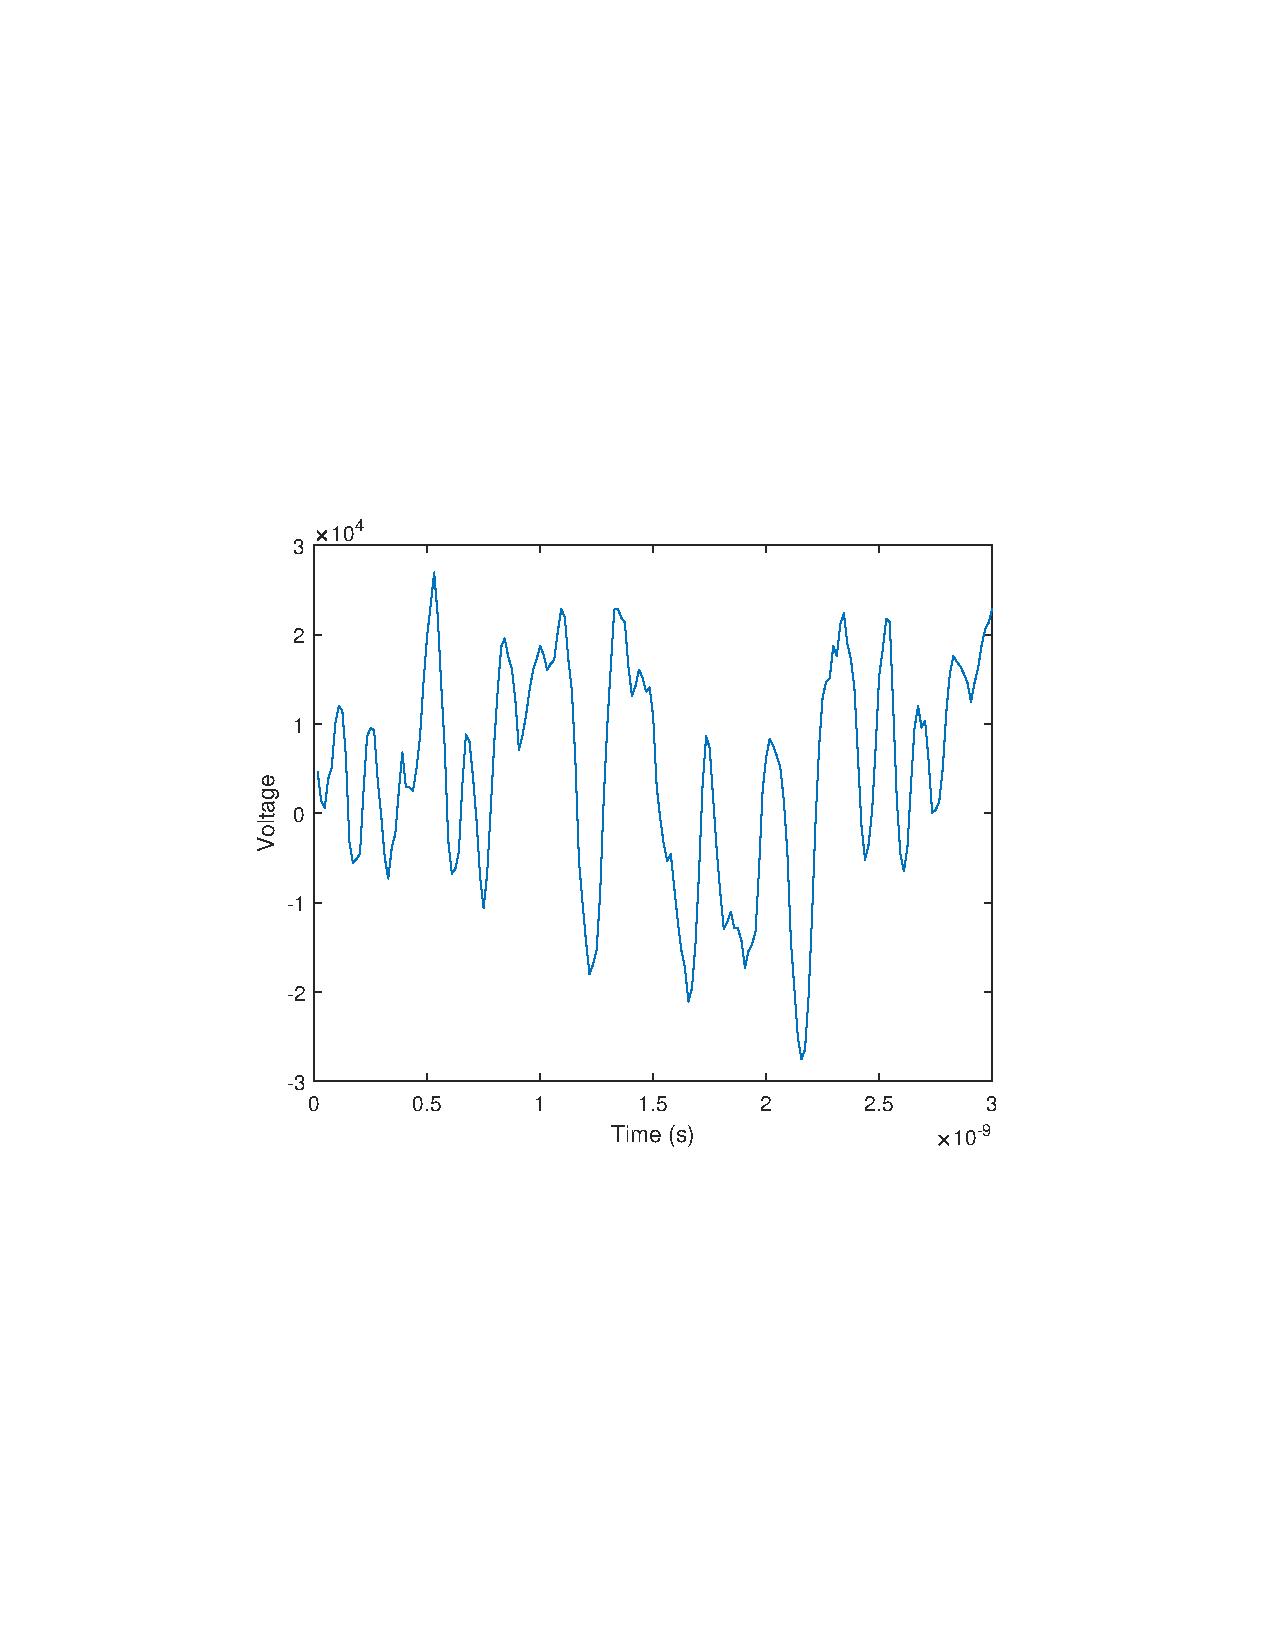
\includegraphics[clip, trim=4cm 8cm 4cm 8cm, width=0.7\textwidth]{./sdf/m_qam_system/figures/exp/RX_03.pdf}
\caption{Signal received at the Oscilloscope (Elec2).}
\label{fig:qamRxSig}
\end{figure}

\begin{figure}[H]
	\centering
	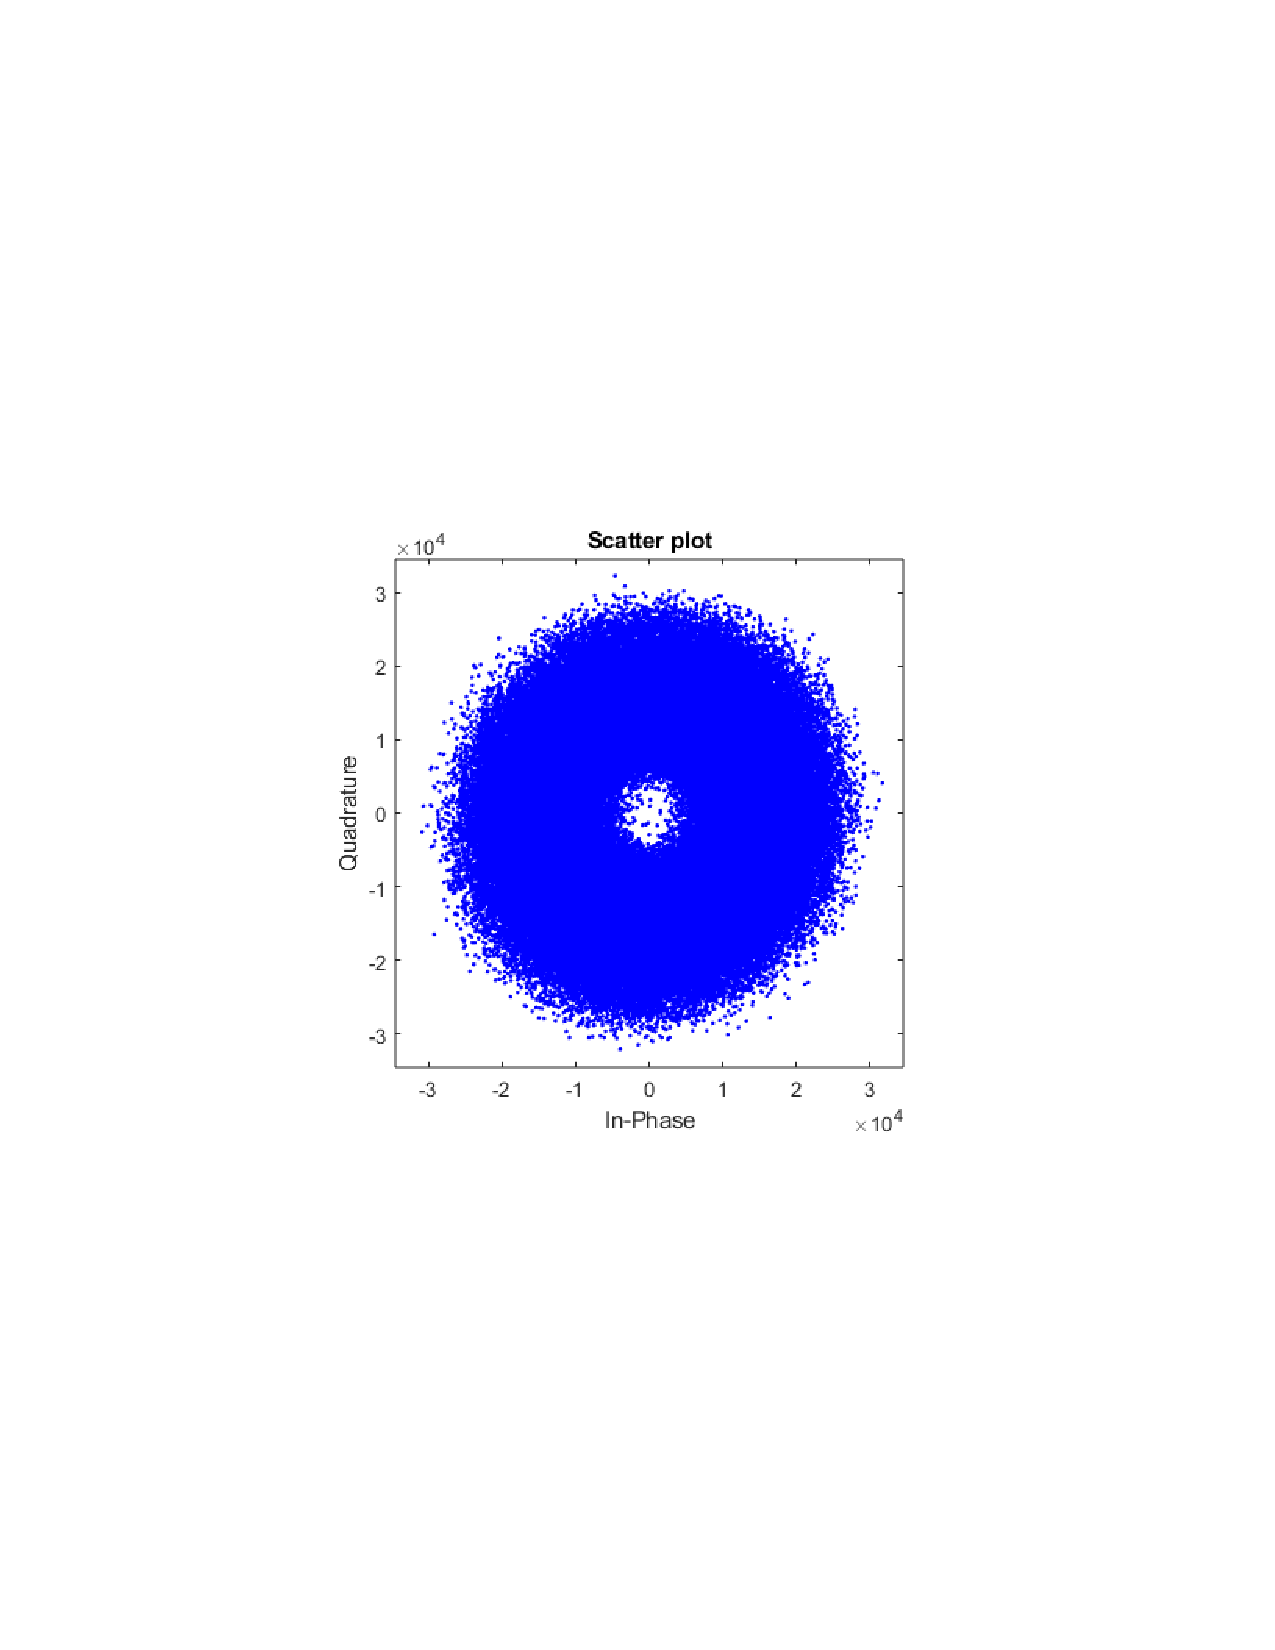
\includegraphics[clip, trim=4cm 8cm 4cm 8cm, width=0.7\textwidth]{./sdf/m_qam_system/figures/exp/const-rtx-sps.pdf}
	\caption{Received constellation without any processing, other than sampling the signal.}
	\label{fig:rxConst}
\end{figure}

The transmitted signal keeps running indefinitely, and the oscilloscope acquires the output of the coherent receiver during a chosen amount of time, which contains several sequences of the signal. Therefore, it is necessary to indentify a single sequence of the signal among the data acquired by the oscilloscope and to align it with the transmitted signal. This was done by measuring the correlation between the data from the oscilloscope and the transmitted signal. The signal was also filtered with a root-raised-cosine FIR.

\begin{figure}[H]
\centering
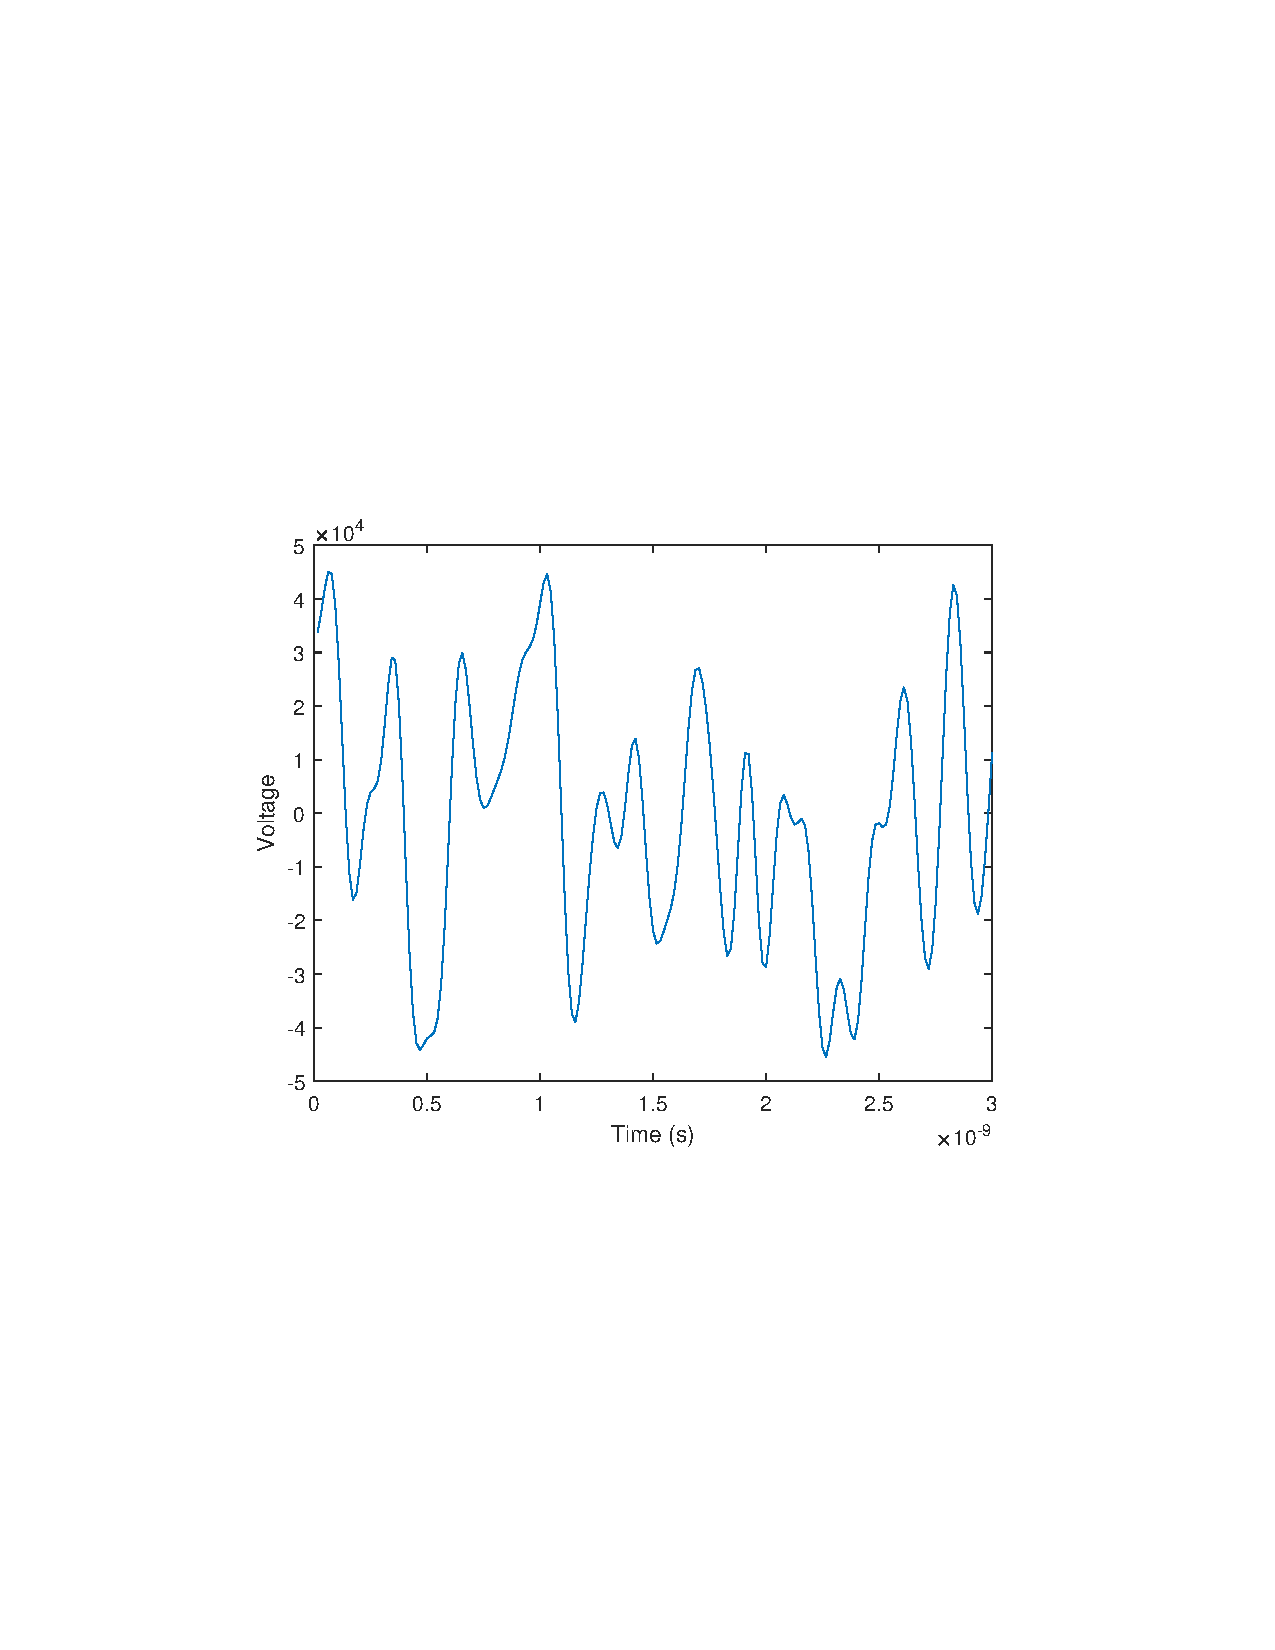
\includegraphics[clip, trim=4cm 8cm 4cm 8cm, width=0.7\textwidth]{./sdf/m_qam_system/figures/exp/MF_03.pdf}
\caption{Signal after digitally applying the root-raised-cosine filter.}
\label{fig:qamMfSig}
\end{figure}

\begin{figure}[H]
	\centering
	\includegraphics[clip, trim=4cm 8cm 4cm 8cm, width=0.7\textwidth]{./sdf/m_qam_system/figures/exp/const-synMF-sps.pdf}
	\caption{Constellation after synchronizing with the transmitted signal, applying the matched filter and truncating the received signal to contain only a single sequence of the transmitted signal.}
	\label{fig:rxMfSync}
\end{figure}

Frequency offset correction was done resorting to a a MATLAB function in the Communication Systems Toolbox, as well as phase correction. To perform phase correction, the constellation was compared with the original constellation (before pulse shaping) and adjusted in order to minimize the differences. The final constellation shown in Figure~\ref{fig:rxFinal}.
%As the data is generated with a Pseudo-Random Number Generator, it is very unlikely that a good result would be

\begin{figure}[H]
	\centering
	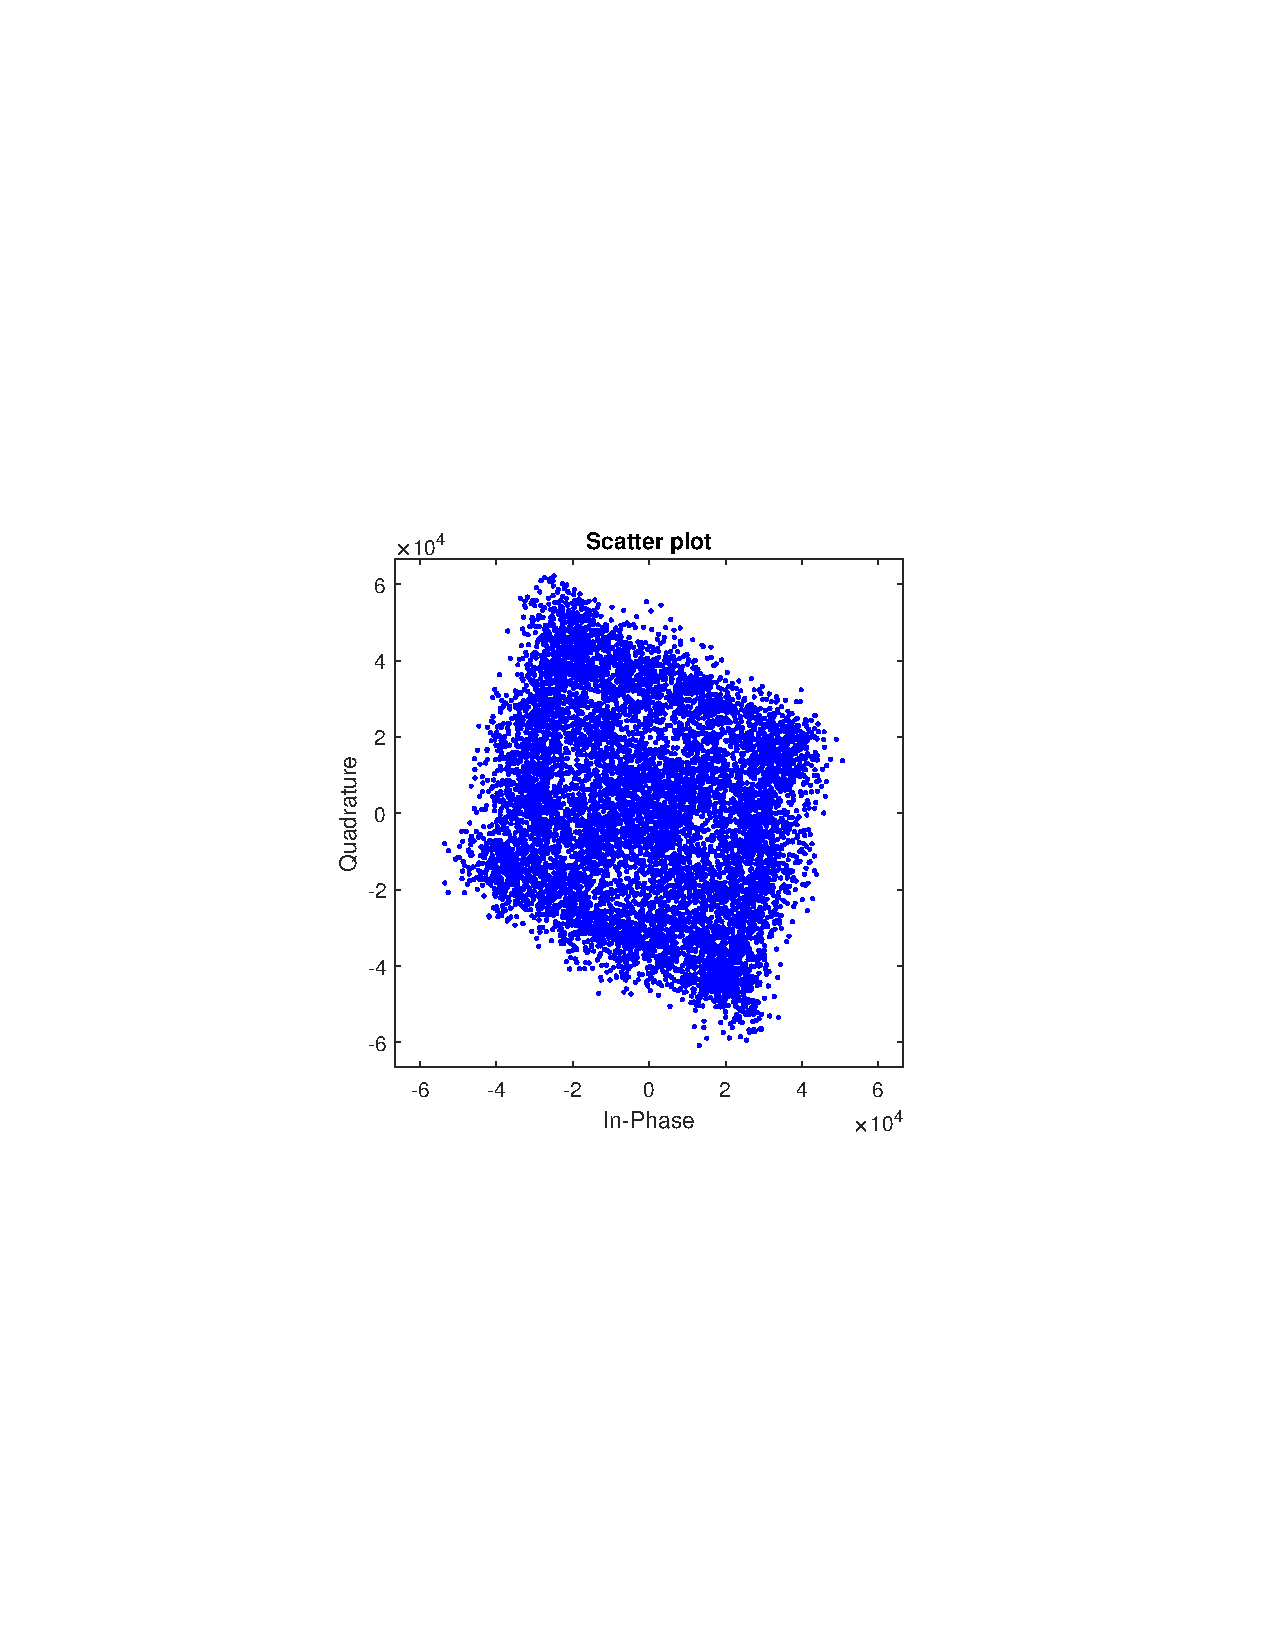
\includegraphics[clip, trim=4cm 8cm 4cm 8cm, width=0.7\textwidth]{./sdf/m_qam_system/figures/exp/const-wvCorr.pdf}
	\caption{Constellation after correcting the frequency offset (without sampling the signal).}
	\label{fig:rxWvCorr}
\end{figure}

\begin{figure}[H]
	\centering
	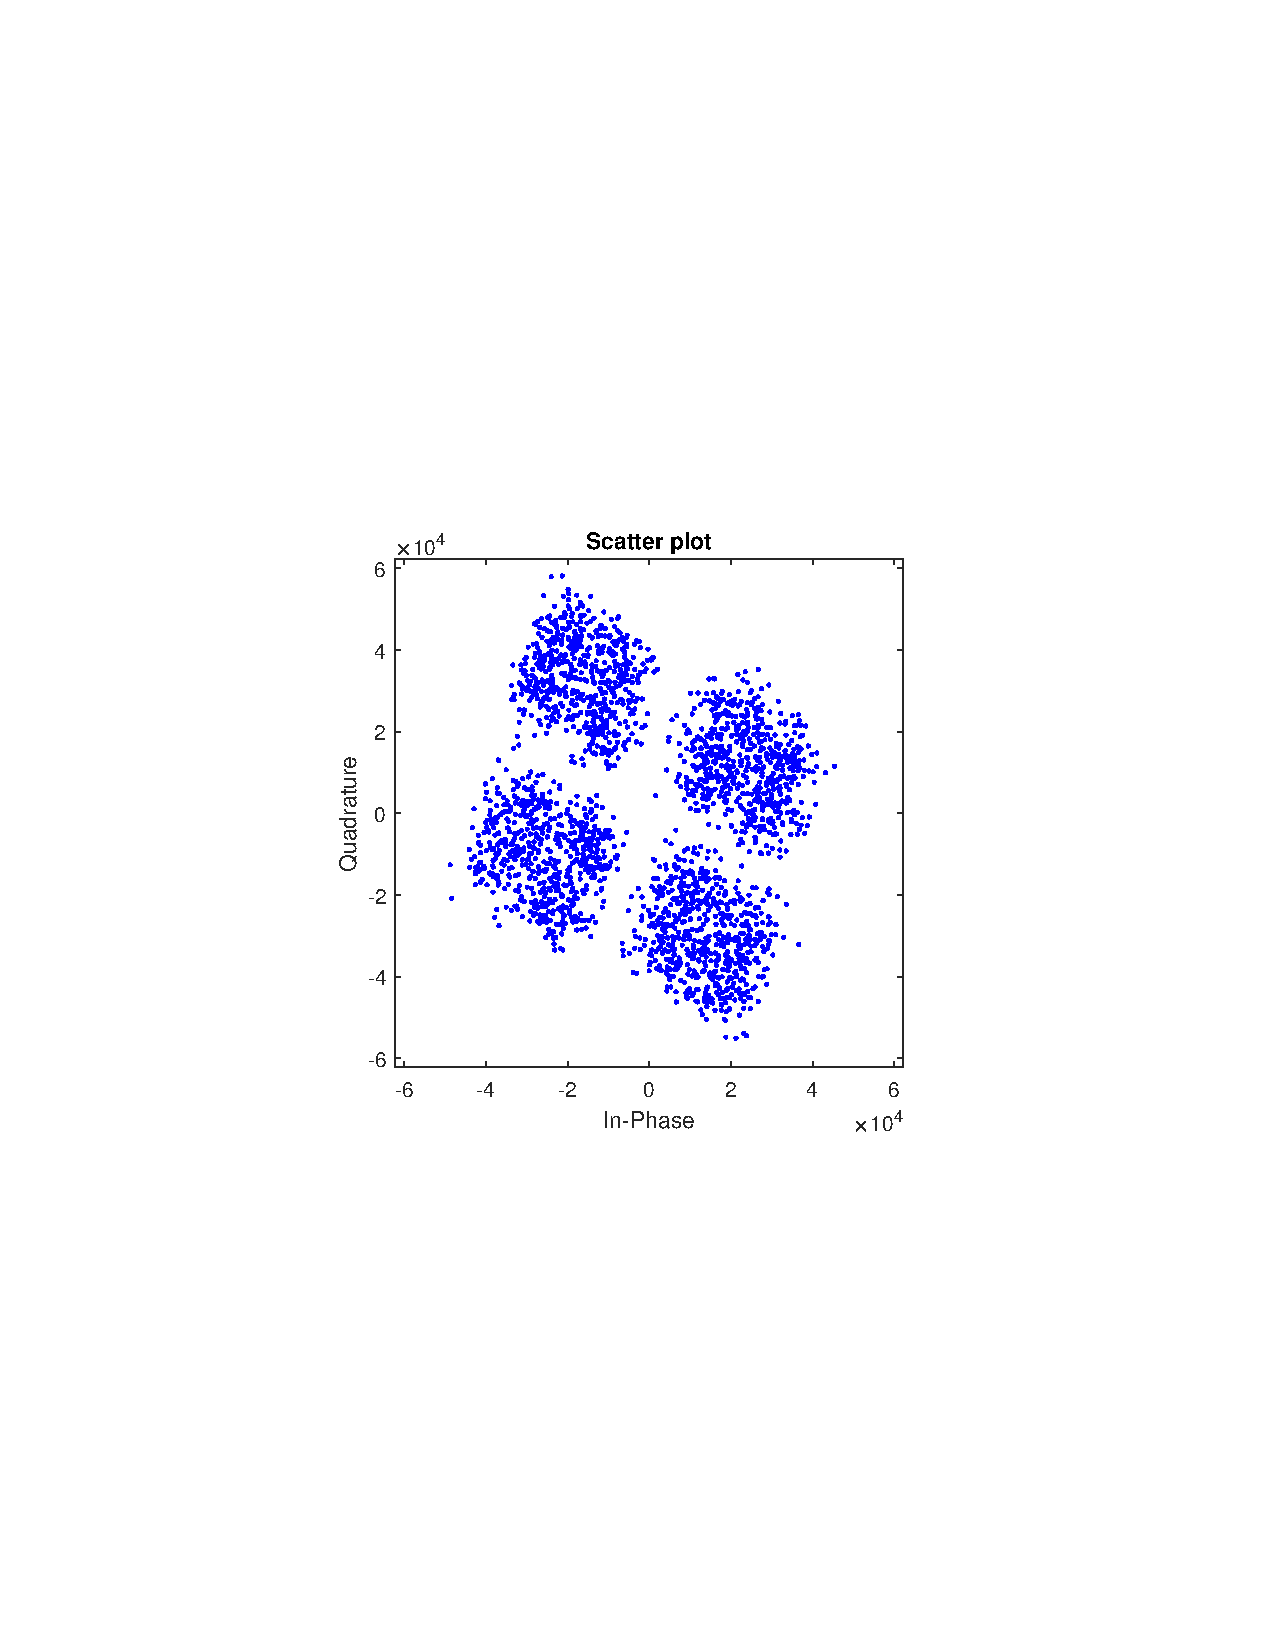
\includegraphics[clip, trim=4cm 8cm 4cm 8cm, width=0.7\textwidth]{./sdf/m_qam_system/figures/exp/const-wvCorr-sps.pdf}
	\caption{Constellation after correcting the frequency offset (after sampling the signal).}
	\label{fig:rxWvCorrSamp}
\end{figure}

\begin{figure}[H]
	\centering
	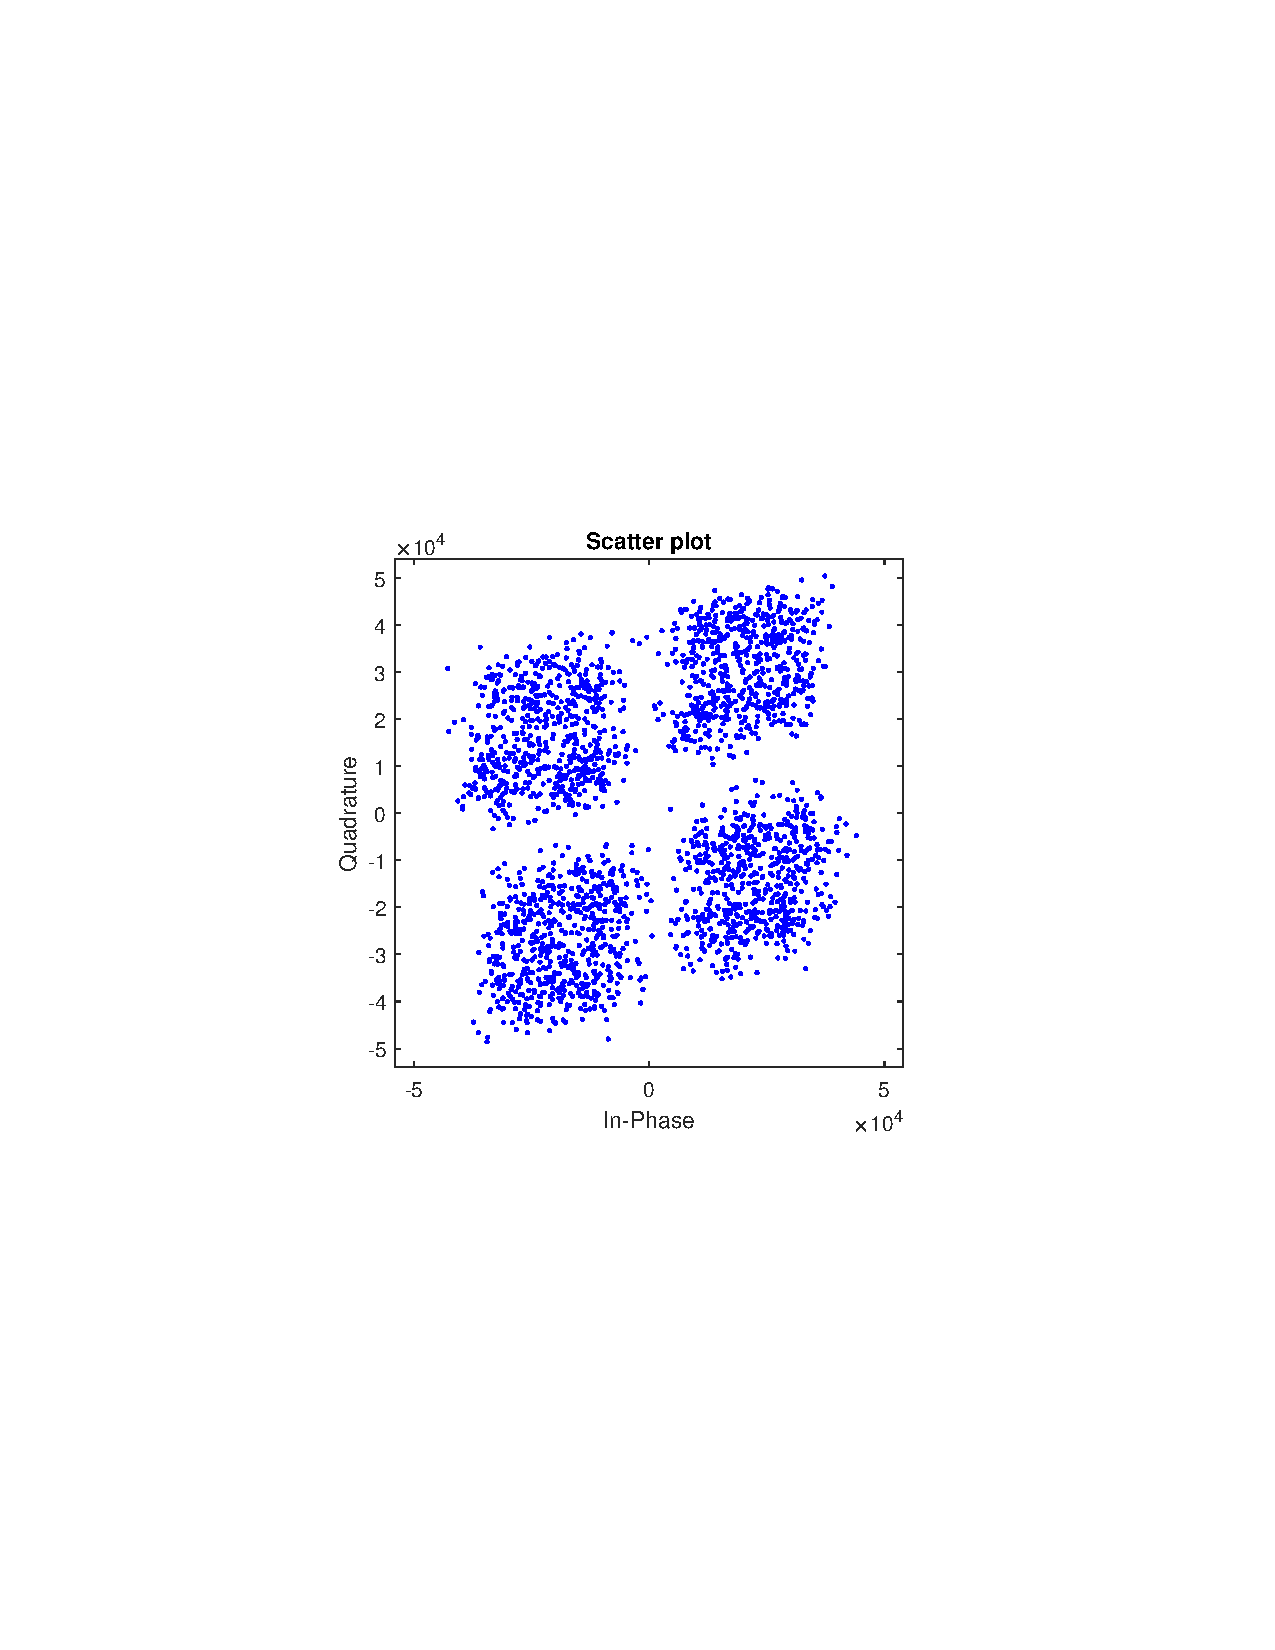
\includegraphics[clip, trim=4cm 8cm 4cm 8cm, width=0.7\textwidth]{./sdf/m_qam_system/figures/exp/const-final-sps.pdf}
	\caption{Constellation after correcting the phase offset.}
	\label{fig:rxFinal}
\end{figure}

As can be seen, the constellation is not properly aligned. Also, the noise seen is far greater than it should be. These issues need to be dealt with before a proper BER curve can be obtained. However, the process so far is somewhat validated by the error rate measurements, which even though they are not proper, are still far from completely wrong or random. The error rate for the shown constellation is around $2 \times 10^{-3}$ for the in-phase component, and around $6 \times 10^{-3}$ for the quadrature component.

\subsection{DSP}

\subsection{Open Issues}

\newpage


%%%%%%%%%%%%%%%%%%%%%%%%%%%%%%%%%%%%%%%%%%%%%%%%%%%%%%%%%%%%%%%%%%%%%%%%%%%%%%%%%%%%%%%%%%%%%%%%%%%%%%%%%%%%
% References
%%%%%%%%%%%%%%%%%%%%%%%%%%%%%%%%%%%%%%%%%%%%%%%%%%%%%%%%%%%%%%%%%%%%%%%%%%%%%%%%%%%%%%%%%%%%%%%%%%%%%%%%%%%%


% bibliographic references for the section ----------------------------
\clearpage
\printbibliography[heading=subbibliography]
\end{refsection}
\addcontentsline{toc}{subsection}{Bibliography}
\cleardoublepage
% ---------------------------------------------------------------------


